\documentclass[oneside,spanish,10pt]{amsart}
\usepackage{setspace}
\usepackage[a4paper]{geometry}
\geometry{verbose,tmargin=2cm,bmargin=2cm,lmargin=2.5cm,rmargin=2.5cm,footskip=1cm,includefoot,headsep=1cm,includehead} % Tamaño
\usepackage{amsthm}
\usepackage[spanish]{babel} % Idioma español
\usepackage[shortlabels]{enumitem} % Mejora el entorno enumerate
\usepackage{graphicx} % Colocar imágenes
\usepackage[hidelinks, colorlinks=true, citecolor=black, linkcolor=., urlcolor=blue]{hyperref} % Vínculos y referencias interactivas
\usepackage{xurl}
\usepackage[skip=3pt]{caption} % Permite modificar el espacio entre el caption y la imagen
\usepackage{multicol} % Entornos de múltiples columnas
\usepackage{nicefrac}
\usepackage{tikz}
\usepackage[center]{titlesec}
\usepackage{titletoc}
\usepackage{pdfpages}
\usepackage{tcolorbox}

%-------------------------------------------------------------------------
% Configuraciones iniciales
\makeatletter
%Numeración
\numberwithin{equation}{section}
\numberwithin{figure}{section}
\newlength{\lyxlabelwidth}      % Longitud auxiliar
\makeatother
%-------------------------------------------------------------------------

%-------------------------------------------------------------------------
% FUENTES
\usepackage[medium]{inter}
\usepackage{mathpazo}
\usepackage{domitian}
\usepackage[T1]{fontenc}
\let\oldstylenums\oldstyle
%-------------------------------------------------------------------------

%-------------------------------------------------------------------------
% Bibliografía
\usepackage[%
backend=biber,
bibstyle=apa,
citestyle=numeric,
sorting=none,
block=none,
maxbibnames=99
]{biblatex}

\defbibheading{bibliography}[\refname]{}

\renewcommand*{\labelalphaothers}{}

\makeatletter
\RequireBibliographyStyle{numeric}
\makeatother

%-------------------------------------------------------------------------
% ARCHIVOS DE BIBLIOGRAFÍAS
\addbibresource{Trabajos/01/refs-01.bib}
\addbibresource{Trabajos/02/refs-02.bib}
\addbibresource{Trabajos/03/refs-03.bib}
\addbibresource{Trabajos/04/refs-04.bib}
\addbibresource{Trabajos/05/refs-05.bib}
\addbibresource{Trabajos/06/refs-06.bib}
\addbibresource{Trabajos/07/refs-07.bib}
\addbibresource{Trabajos/08/refs-08.bib}
\addbibresource{Trabajos/09/refs-09.bib}
\addbibresource{Trabajos/10/refs-10.bib}
\addbibresource{Trabajos/11/refs-11.bib}
\addbibresource{Trabajos/12/refs-12.bib}
\addbibresource{Trabajos/13/refs-13.bib}
\addbibresource{Trabajos/14/refs-14.bib}
\addbibresource{Trabajos/15/refs-15.bib}
\addbibresource{Trabajos/16/refs-16.bib}
%-------------------------------------------------------------------------

%-------------------------------------------------------------------------
% Otras configuraciones
\addto\captionsspanish{\renewcommand{\tablename}{Tabla}}
\addto\captionsspanish{\renewcommand{\figurename}{Figura}}

\theoremstyle{definition}
\newtheorem{actividad_previa}{\normalfont ACTIVIDAD PREVIA}
\newtheorem{actividad}{\normalfont ACTIVIDAD}
\newtheorem{actividad_entre}{\normalfont ACTIVIDAD ENTRE CLASES}
\newtheorem*{evaluacion}{\normalfont EVALUACIÓN}
\newtheorem*{observacion}{Observacion}
\newtheorem*{teorema}{Teorema}
%-------------------------------------------------------------------------

\usepackage{fancyhdr}
\pagestyle{fancy}
\renewcommand{\headrulewidth}{0pt}
\fancyhead[C]{\scshape Memorias de las VIII JEM - 2024\\ \vspace{1mm} \hrule \vspace{1mm}
	\scshape\scriptsize \articulotitulocorto}
\fancyhead[L]{}
\fancyhead[R]{\vspace{1em}\small\scshape\articulotipo}
\fancyfoot[C]{\small \thepage}

\fancypagestyle{portadapage}{
	\fancyhf{}
	\renewcommand{\headrulewidth}{0pt}
	\fancyhead[C]{\scshape Memorias de las VIII JEM - 2024}
	\fancyhead[R]{\small\scshape\articulotipo}
	\fancyfoot[C]{\small \thepage}
}

%-------------------------------------------------------------------------
% TABLA DE CONTENIDOS
\setcounter{tocdepth}{1}
\newcommand{\desctotoc}[1]{%
	\addtocontents{toc}{\hspace*{3em}\medskip\detokenize{\textit{#1}}\leavevmode\par\medskip}
}
%-------------------------------------------------------------------------

%-------------------------------------------------------------------------
% TÍTULOS DE SECCIONES
\setcounter{secnumdepth}{4}
\titleformat{\section}[block]{\centering\setstretch{0.75}\Huge\scshape}{}{1em}{}
\titleformat{\subsection}{\centering\scshape}{\arabic{subsection}.}{1em}{\LARGE}
\titleformat{\subsubsection}{\normalfont\bfseries}{\arabic{subsection}.\arabic{subsubsection}}{1em}{\large}
\titleformat{\paragraph}{\normalfont\bfseries}{\arabic{subsection}.\arabic{subsubsection}.\arabic{paragraph}}{1em}{\large}
\titlespacing*{\paragraph}{0pt}{1em}{1em}

\titlecontents{section}
[3em] % indentación desde margen izquierdo
{\vspace{2pt}} % formato antes de la entrada (puedes dejar vacío {})
{\contentslabel{1.5em}} % formato del número (ancho reservado)
{} % formato sin número (si no tiene)
{\hfill\contentspage} % formato del número de página alineado a la derecha


%-------------------------------------------------------------------------

%-------------------------------------------------------------------------
% QUOTING
\let\oldquote\quote \renewcommand\quote{\oldquote\small}
%-------------------------------------------------------------------------

%-------------------------------------------------------------------------
% REFERENCIAS
\renewcommand{\thesubsubsection}{\arabic{subsection}.\arabic{subsubsection}}
%-------------------------------------------------------------------------

%-------------------------------------------------------------------------
% AUTORES
\newcommand{\addautor}[3][]{%
	{\Large \scshape #2}\\%
	{\large \itshape #3}\\%
	\ifx\\#1\\%
	% Si el argumento opcional (correo) está vacío, no hace nada
	\else
	{\ttfamily \small #1}\\%
	\fi
}
%-------------------------------------------------------------------------

%-------------------------------------------------------------------------
% DOCUMENTO

\title{}
\author{}
\date{}
\newcommand{\articulotitulo}{}
\newcommand{\articulotitulocorto}{}
\newcommand{\articulotipo}{}

\begin{document}
	
	% Toda la primer parte
	
\includepdf{Trabajos/Portada.pdf}
	\clearpage
	\begin{center}
	\LARGE \bfseries \sffamily
	Memorias de las VI Jornadas de Enseñanza de la Matemática (JEM)
\end{center}

\vspace*{2.5mm}

\begin{center}
	\begin{tcolorbox}[colback=white, arc=0mm, width=10cm, boxrule=0.5pt]
		\footnotesize
		Universidad Nacional de Salta
		
		\hspace*{1em} Memorias de las VI Jornadas de Enseñanza de la Matemática (JEM) / Compilado por Sángari, Antonio Noé - Salta: Universidad Nacional de Salta, 2023.
		
		\vspace*{1em}
		
		\hspace*{1em} Archivo digital: descarga y online
		
		\hspace*{1em} ISBN 978-987-633-615-4		
	\end{tcolorbox}
\end{center}

\vspace*{2.5mm}

\begin{center}
	\sffamily \Large \bfseries Compiladores
	
	\large \normalfont
	Guzmán González, Ramiro 
	
	Sángari, Antonio Noé 
\end{center}

\begin{center}
	\sffamily \Large \bfseries Revisores de talleres y comunicaciones breves
	
	\vspace*{-1em}
	
	\begin{multicols}{2}
		\large \normalfont
		Alberto, Diego Luis
		
		Aliendro, Estela Sonia
		
		Arias, Jesús Eduardo
		
		Ávila, Mario Ubaldo
		
		Bifano, Fernando Jorge  
		
		Duarte, Betina
		
		Etchegaray, Silvia Catalina
		
		Ferrero, María Martha 
		
		Formeliano, Blanca Azucena 
		
		Funes, Héctor Nicolás
		
		García, José Ignacio
		
		Martínez, Rosa
		
		Marrón, Beatriz Susana
		
		Méndez, Nilda Graciela
		
		Mercau, Beatriz Susana
		
		Oliva, Elisa
		
		Quintana, Pablo
		
		Rodríguez, Mabel Alicia
		
		Roig, María Eugenia 
		
		Rosales, Juan Carlos
		
		Puca, Silvana Mercedes del Milagro 
		
		Saidón, Liliana
		
		Sángari, Antonio Noé 
		
		Micelli, Mónica Lorena
		
		Torres, Germán Ariel
		
		Villagra, Celia Elizabeth
		
		Villarreal Cantizana, Claudia
		
		Viola, Fernanda Beatriz 
		
		Yazlle, Jorge Fernando
	\end{multicols} 
\end{center}

\begin{center}
	\sffamily \Large \bfseries Maquetación
	
	\large \normalfont
	Martinez, Gonzalo Matias
\end{center}

\begin{center}
	\sffamily \Large \bfseries Diseño e identidad
	
	\large \normalfont
	Díaz, Aldana Lucía
\end{center}

\vspace*{2.5mm}

\begin{center}
	\scshape \Large Universidad Nacional de Salta
	
	\normalfont \normalsize
	Av. Bolivia 5150 -- Salta Capital
\end{center}

\vfill

\begin{center}
	\footnotesize
	Queda prohibida la reproducción total o parcial del texto de la presente obra en cualquiera de sus formas, electrónica o mecánica, sin el consentimiento previo y escrito del autor.
\end{center}
	\clearpage
	\begin{center}
	\LARGE \bfseries \sffamily Autoridades
\end{center}

\begin{center}
	\sffamily \Large \bfseries Universidad Nacional de Salta

	\bigskip
	
	\sffamily \large \bfseries Rector
	
	\normalfont \large
	Ing. Daniel HOYOS
	
	\bigskip
	
	\sffamily \large \bfseries Vicerrector
	
	\normalfont \large
	Cr. Nicolás INNAMORATO
	
	\bigskip
	
	\sffamily \large \bfseries Secretario de Extensión 
	
	\normalfont \large
	Lic. Rubén Emilio CORREA
\end{center}

\vspace*{5mm}

\begin{center}
	\sffamily \Large \bfseries Facultad de Ciencias Exactas
	
	\bigskip
	
	\sffamily \large \bfseries Decano
	
	\normalfont \large
	Mg. Gustavo Daniel GIL
	
	\bigskip
	
	\sffamily \large \bfseries Vicedecana
	
	\normalfont \large
	Dra. María Rita MARTEARENA
\end{center}

\vspace*{5mm}

\begin{center}
	\sffamily \Large \bfseries Departamento de Matemática
	
	\bigskip
	
	\sffamily \large \bfseries Directora
	
	\normalfont \large
	Lic. María Cristina AHUMADA
	
	\bigskip
	
	\sffamily \large \bfseries Secretario
	
	\normalfont \large
	Prof. Juan Pablo DIOLI
	
	\bigskip
	
	\sffamily \large \bfseries Prosecretario
	
	\normalfont \large
	Mg. Héctor Nicolás FUNES
\end{center}
	\clearpage
	\begin{center}
	\LARGE \bfseries \sffamily Equipo Editorial JEM
\end{center}

\begin{center}
	\sffamily \Large \bfseries Coordinación General
	
	\bigskip
	
	\normalfont \large
	Prof. Silvia Mabel Baspiñeiro
	
	Prof. Blanca Azucena Formeliano
	
	Prof. lvone Anahí Patagua
	
	Prof. Antonio Noé Sángari
\end{center}

\vspace*{2.5mm}

\begin{center}
	\sffamily \Large \bfseries Plataforma
	
	\bigskip
	
	\sffamily \large \bfseries Open Journal System (OJS)
	
	\normalfont \large
	Lic. Ramiro Guzmán González
	
	\bigskip
	
	\sffamily \large \bfseries Diseño de Identidad
	
	\normalfont \large
	Lic. Aldana Lucía Díaz
	
	\bigskip
	
	\sffamily \large \bfseries Maquetación 
	
	\normalfont \large
	Gonzalo Matias Martinez
\end{center}

\vspace*{5mm}

\begin{center}
	\sffamily \Large \bfseries Declaraciones de Interés Educativo y Avales Institucionales
	
	\bigskip
	
	\normalfont \normalsize \scshape
	Rectorado
	
	Universidad Nacional de Salta
	
	RES. R. N° 937/2022
	
	\bigskip
	
	Facultad de Ciencias Exactas 
	
	Universidad Nacional de Salta
	
	RESD-EXA N° 379/2022
	
	\bigskip
	
	Ministerio de Educación, Cultura, Ciencia 
	
	y Tecnología de la Provincia de Salta
	
	RES. N° 128/2022
	
\end{center}
	\clearpage
	\section*{\centering \sffamily Prólogo}

Las VII Jornadas de Enseñanza de la Matemática híbridas, realizadas en su parte presencial en las instalaciones de la Universidad Nacional de Salta del 24 de julio al 2 de agosto de 2023, representaron un hito en el continuo esfuerzo por mejorar la calidad de la educación matemática en nuestra región. Durante esos días, docentes, investigadores y estudiantes se congregaron con el objetivo de reflexionar sobre sus prácticas docentes, compartiendo experiencias y conocimientos que, sin duda, contribuirán al enriquecimiento de la comunidad educativa.

Las Jornadas ofrecieron un variado programa de actividades que incluyó conferencias magistrales, talleres prácticos y comunicaciones breves. Entre las actividades destacadas, se encuentran las conferencias de Valeria Borsani, que abordó \emph{El pasaje de la aritmética al álgebra en los primeros años de la escuela media}, la de Andrés Rieznik, que abordó \emph{Discalculia, un capítulo olvidado de la neuropsicología}, y el de Daniela Reyes, \emph{Empoderamiento docente, ¿por qué pensar en ello?} y cinco talleres sobre enseñanza de la matemática. La participación activa de los asistentes reflejó el interés y el compromiso con la mejora continua de la enseñanza de la matemática.

Queremos expresar nuestro más sincero agradecimiento a todos los participantes, ponentes y talleristas que, con su dedicación y entusiasmo, hicieron posible el éxito de este evento. Asimismo, extendemos nuestro reconocimiento a la Universidad Nacional de Salta y a todas las instituciones que nos brindaron su apoyo.

Las presentes Memorias recogen las ideas, debates y conclusiones surgidas durante las Jornadas, sirviendo como un valioso recurso para todos aquellos interesados en la enseñanza de la matemática. Esperamos que este compendio inspire a los lectores a continuar explorando y aplicando nuevas estrategias pedagógicas en sus aulas.

Con la mirada puesta en el futuro, confiamos en que las próximas ediciones de las Jornadas de Enseñanza de la Matemática seguirán siendo un espacio de encuentro, reflexión e innovación para nuestra comunidad.

\vspace{5cm}

\begin{center}
	\large Prof. Antonio Noé Sángari
	
	\normalfont Coordinador de las VII Jornadas de Enseñanza de la Matemática
\end{center}
	\clearpage
	\thispagestyle{portadapage}
\tableofcontents
	\clearpage
	\thispagestyle{portadapage}
\renewcommand{\articulotipo}{}

\vspace*{\fill}
\begin{center}
	\sffamily \bfseries \LARGE I
	
	\Huge Talleres
\end{center}
\vspace*{\fill}
\addcontentsline{toc}{part}{I \hspace*{1em} Talleres}
	\clearpage
	%-------------------------------------------------------------------------
% INFORMACIÓN DEL ARTÍCULO
\thispagestyle{portadapage}
\setcounter{subsection}{0}
\setcounter{subsubsection}{0}
\setcounter{actividad}{0}
\setcounter{actividad_previa}{0}
\setcounter{actividad_entre}{0}
\renewcommand{\articulotipo}{Taller}
\renewcommand{\articulotitulo}{Preparación de estudiantes para las Olimpiadas Matemáticas: Técnicas de preparación}
\renewcommand{\articulotitulocorto}{Preparación de estudiantes para las Olimpiadas Matemáticas: Técnicas de preparación}
\section{\articulotitulo}
\desctotoc{Sángari, A. N.; Flores Rocha, V.; Ghiglia, N. N.; Coria, S. E.}

\noindent\rule{\linewidth}{2pt}

\vspace{0.25cm}

\begin{flushright}
	{\Large \scshape
		Antonio Noé Sángari
	}\\
	{\large \itshape
		Universidad Nacional de Salta
	}\\
	{\ttfamily \small
		diamantecinthia@gmail.com
	}\\
	\vspace{1em}
	{\Large \scshape
		Veronica Flores Rocha
	}\\
	{\large \itshape
		Universidad Nacional de Salta
	}\\
	\vspace{1em}
	{\Large \scshape
		Nadia Noel Ghiglia
	}\\
	{\large \itshape
		Universidad Nacional de Salta
	}\\
	\vspace{1em}
	{\Large \scshape
		Silvia Ester Coria
	}\\
	{\large \itshape
		Universidad Nacional de Salta
	}
\end{flushright}

\vspace{0.5cm}

\begin{center}
	\begin{minipage}{0.75\linewidth} \small
		\textsc{Resumen}. ~
		Este curso-taller está diseñado para capacitar a docentes de matemáticas de secundaria en técnicas de demostración matemática, con el objetivo de preparar a sus estudiantes para participar en las Olimpiadas Matemáticas. Se enfocará en el desarrollo de habilidades de razonamiento lógico y deductivo, la enseñanza de estrategias didácticas específicas y la aplicación de estos conocimientos en la práctica. Los participantes tendrán acceso a materiales teóricos, actividades prácticas y herramientas de evaluación para asegurar un aprendizaje integral.
	\end{minipage}
	
	\vspace{0.5em}
	
	\begin{minipage}{0.75\linewidth} \small
		\textsc{Palabras clave} --- Curso-taller, Matemáticas, Olimpiadas Matemáticas, Razonamiento lógico, Razonamiento deductivo.
	\end{minipage}
\end{center}
%-------------------------------------------------------------------------

\subsection{Introducción}

\subsubsection{Sobre el taller}

El curso-taller «Preparación de Estudiantes para las Olimpiadas Matemáticas: Técnicas de Demostración» está diseñado específicamente para docentes de matemáticas de nivel secundario. Este programa tiene como objetivo principal dotar a los profesores de las herramientas y estrategias necesarias para enseñar a sus estudiantes a construir demostraciones matemáticas rigurosas. La habilidad de realizar demostraciones precisas es un aspecto crucial en las Olimpiadas Matemáticas, con un énfasis particular en la geometría básica.

En el contexto de las Olimpiadas Matemáticas, tanto a nivel nacional como internacional, la capacidad de los estudiantes para presentar demostraciones claras y lógicas es fundamental para su éxito. Por esta razón, el curso-taller pone un énfasis especial en proporcionar a los docentes un sólido soporte bibliográfico a través de la Red Olímpica. Esta red ofrece una guía valiosa para las demostraciones esperadas en las competiciones, ayudando a los estudiantes a prepararse adecuadamente y a competir con confianza en los diferentes niveles de las Olimpiadas.

Con este curso-taller, se espera que los docentes adquieran un mayor dominio en la enseñanza de técnicas de demostración y, a su vez, transmitan estos conocimientos a sus alumnos, potenciando así sus habilidades matemáticas y su desempeño en las competiciones.

\subsubsection{Importancia de la enseñanza de la demostración}

Destacamos que en el contexto de la Olimpiada Matemática Argentina, la demostración ocupa un lugar central y fundamental en la resolución de problemas matemáticos. A diferencia de las respuestas simples o los cálculos rápidos, una demostración matemática exige un razonamiento riguroso y lógico.

La demostración es esencial en la Olimpiada Matemática porque asegura la validez de las soluciones, desarrolla habilidades críticas y analíticas, promueve una comunicación efectiva, profundiza la comprensión matemática y permite una evaluación justa y completa de las capacidades
de los estudiantes.

\subsection{Contenidos}

\subsubsection{Módulo 1: Definición y tipos de demostraciones.}
\begin{itemize}
	\item Elementos de una demostración rigurosa.
	\item Ejemplos históricos y su importancia.
	\item Ejemplos de certámenes nacionales e internacionales de la Olimpiada Matemática Argentina, tanto en soporte bibliográfico como en publicación en linea.
	\item Estrategias didácticas para enseñar estos conceptos.
\end{itemize}

\subsubsection{Módulo 2: Técnicas Básicas de Demostración}
\begin{itemize}
	\item Demostraciones directas.
	\item Demostraciones por contradicción.
	\item Demostraciones por contraposición.
	\item Ejercicios prácticos y resolución de problemas.
	\item Métodos para enseñar estas técnicas a los estudiantes.
\end{itemize}

\subsubsection{Módulo 3: Geometría}
\begin{itemize}
	\item Postulados y teoremas fundamentales.
	\item Construcción de demostraciones geométricas.
	\item Aplicación de teoremas en problemas de Olimpiadas en certámenes regionales, nacionales e internacionales.
	\item Actividades prácticas.
\end{itemize}

\subsection{Requisitos previos}

Docentes de matemáticas de nivel secundario y estudiantes avanzados de profesorados de matemática, interesados en preparar a sus estudiantes para participar en Olimpiadas Matemáticas.

\subsection{Objetivos}
\begin{enumerate}
	\item Capacitar a los docentes en técnicas de demostración matemática.
	\item Fomentar habilidades de razonamiento lógico y deductivo en sus estudiantes.
	\item Proveer estrategias didácticas para enseñar demostraciones.
	\item Preparar a los docentes para guiar a sus estudiantes en competiciones matemáticas regionales, nacionales e internacionales.
\end{enumerate}

\subsection{Actividades}

\subsubsection{Actividades previas}

Antes del inicio formal del curso-taller, los participantes tendrán acceso a un curso en la plataforma Moodle de la Facultad de Ciencias Exactas. En esta plataforma, se adjuntarán extractos esenciales de elementos de una prueba en matemática, especialmente del texto de \textcite{margaris1968} sobre lógica formal como soporte básico y del clásico de \textcite{polya1945} sobre resolución de problemas y organización de demostraciones. Además, se proporcionarán videos explicativos que cubren demostraciones básicas para familiarizar a los docentes con los conceptos fundamentales. El programa y el cronograma detallado de actividades del curso estarán disponibles en la plataforma, permitiendo a los participantes planificar su tiempo de estudio. Para asegurar que los docentes asimilen los conceptos preliminares, se implementará un cuestionario de autoevaluación, el cual los participantes deberán completar antes de la primera sesión sincrónica.

\subsubsection{Primeras hora y media sincrónicas}

La primera sesión sincrónica comenzará con una breve presentación del taller, estableciendo los objetivos y la estructura del curso. Se introducirán las ideas básicas de los elementos de una demostración, proporcionando una visión general de los conceptos fundamentales que serán abordados en profundidad más adelante. Se solicitará la participación activa de los cursantes, quienes serán invitados a compartir sus perspectivas y experiencias sobre la enseñanza de demostraciones matemáticas. Esta discusión inicial ayudará a identificar los conocimientos previos de los docentes y a ajustar el enfoque del taller según sus necesidades.

\subsubsection{Primeras tres horas entre clases}

Estas horas estarán
dedicadas a la preparación de las próximas clases sincrónicas centradas en el módulo 2, que aborda diversos métodos de demostración y técnicas para enseñarlos. Se pondrán a disposición textos extraídos del libro de \textcite{larson1983} sobre resolución de problemas para estructurar los métodos de demostración. Adicionalmente, se seleccionarán problemas relevantes de los libros de \textcite{araujo2020a, araujo2020b, araujo2020c, fauring2000, fauring2023}, los cuales serán utilizados como ejemplos prácticos durante las sesiones sincrónicas. Los participantes deberán revisar estos materiales y reflexionar sobre su aplicación en el aula, preparando preguntas y comentarios para la próxima sesión.

\subsubsection{Segundas hora y media sincrónicas}

En esta sesión, se abordará el módulo 2 siguiendo una metodología similar a la de las primeras horas sincrónicas. El enfoque estará en las técnicas básicas de demostración y en métodos pedagógicos para enseñar estas técnicas a los estudiantes. Los cursantes serán invitados a explicar el material que se les asignó para lectura durante las primeras tres horas entre clases, fomentando así una discusión profunda y colaborativa. Se debatirán posibles modificaciones a los ejercicios presentados para obtener respuestas más generales y abarcativas, permitiendo a los docentes adaptar los problemas a diferentes niveles de dificultad y contextos de enseñanza.

\subsubsection{Segundas tres horas entre clases}

Durante estas horas, los participantes prepararán las próximas clases sincrónicas que continuarán con el módulo 3. Este módulo se centrará en la justificación de las hipótesis y en el camino lógico necesario para obtener los teoremas más comunes en la geometría elemental. Se proporcionarán materiales adicionales que exploran estos conceptos en profundidad, incluyendo ejemplos prácticos y ejercicios para resolver. Los docentes deberán revisar estos materiales y preparar sus propias explicaciones y preguntas para la próxima sesión sincrónica, asegurando así una comprensión sólida de los temas tratados.

\subsubsection{Terceras hora y media sincrónicas}

La tercera sesión sincrónica continuará con el módulo 3, siguiendo el mismo enfoque interactivo y participativo de las sesiones anteriores. Se profundizará en las técnicas de demostración y resolución de problemas, con un énfasis especial en la búsqueda de primeros principios para fundamentar los resultados obtenidos. Se dedicará la parte final de esta sesión a explicar la evaluación final del curso-taller, aclarando cualquier duda que los participantes puedan tener. Esto asegurará que todos los cursantes estén bien preparados para demostrar su comprensión y aplicación de las técnicas de demostración matemática enseñadas a lo largo del taller.

\subsubsection{Evaluación final}

\begin{itemize}
	\item Desarrollo de recursos educativos para el entrenamiento de estudiantes, centrados en el razonamiento lógico de deducciones geométricas.
	\item Cuestionario final que aborde los principales temas del taller.
	\item Reflexión escrita sobre la experiencia del taller y el aprendizaje obtenido.
\end{itemize}

\subsection{Bibliografía}

\nocite{*}
\printbibliography[keyword={01}]
	\clearpage
	%-------------------------------------------------------------------------
% INFORMACIÓN DEL ARTÍCULO
\thispagestyle{portadapage}
\setcounter{subsection}{0}
\setcounter{subsubsection}{0}
\setcounter{actividad}{0}
\setcounter{actividad_previa}{0}
\setcounter{actividad_entre}{0}
\renewcommand{\articulotipo}{Taller}
\renewcommand{\articulotitulo}{Datos educativos: producción y uso de herramientas de procesamiento de información con asistencia de la IA para la toma de decisiones}
\phantomsection
\stepcounter{section}
\addcontentsline{toc}{section}{\protect\numberline{\thesection} \articulotitulo}
\desctotoc{Villagra, C. E.; Miguez, I. H; Acosta, R. N.; Chorolque, E. M.}

\begin{center}
	\setstretch{1.5}
	{\Huge \scshape 
		\articulotitulo
	}
\end{center}

\noindent\rule{\linewidth}{2pt}

\vspace{0.25cm}

\begin{flushright}
	{\Large \scshape
		Fernando Jorge Bifano
	}\\
	{\large \itshape
		Facultad de Ciencias Exactas y Naturales — Universidad de Buenos Aires
	}\\
	{\ttfamily \small
		fjbifano@ccpems.exactas.uba.ar
	}\\
	\vspace{1em}
	{\Large \scshape
		Pablo Fabián Carranza
	}\\
	{\large \itshape
		Universidad Nacional de Río Negro
	}\\
	\vspace{1em}
\end{flushright}

\vspace{0.5cm}

\begin{center}
	\begin{minipage}{0.75\linewidth} \small
		\textsc{Resumen}. ~
		La generación y uso de datos es actualmente uno de los nuevos emergentes que impactan en las diferentes esferas de la sociedad y por tanto, la educación se ve tensionada por las demandas que ello conlleva. En ese sentido, surgen nuevas vacancias para la formación docente y se vuelve necesario ofrecer instancias que permitan a quienes enseñan contar con herramientas para la comprensión, uso y toma de decisiones fundadas y sostenidas en la interpretación de la información. Este taller ofrece la posibilidad de familiarizarse con herramientas básicas que brindan los softwares para el procesamiento de la información y que con la asistencia de las IA se ven potenciados en sus aplicaciones. A partir del trabajo con distintos tipos de bases de datos educativos, propondremos un recorrido que aborda algunas herramientas de representación gráfica de la información en lenguaje de programación Python asistido por medio de inteligencias artificiales tales como ChatGPT y Gemini. Se analizarán las potencialidades de estrategias tales como clustering y árboles de decisión para la caracterización de grupos de estudiantes.
	\end{minipage}
	
	\vspace{0.5em}
	
	\begin{minipage}{0.75\linewidth} \small
		\textsc{Palabras clave} --- Datos educativos, IA, Python, Procesamiento de la información.
	\end{minipage}
\end{center}
%-------------------------------------------------------------------------

\subsection{Introducción}

El análisis de datos es una disciplina que ha visto incrementado su desarrollo recientemente por varios factores vinculados entre sí. Entre ellos destacamos:

\begin{itemize}
	\item Disponibilidad de herramientas de procesamiento de datos en computadoras de escritorio.
	\item Crecimiento de librerías de libre acceso en lenguaje Python.
	\item Desarrollo de nuevos métodos de análisis de datos, llegando incluso a herramientas vinculadas a la inteligencia artificial.
	\item Existencia de volúmenes de datos.
\end{itemize}

Estos elementos combinados permiten la aplicación de herramientas que facilitan la comprensión de fenómenos complejos y la toma de decisiones basadas en información.

Las instituciones educativas no escapan a estos avances. En efecto, los datos disponibles o factibles de ser obtenidos permiten una mejor interpretación de fenómenos del ecosistema educativo y el desarrollo de acciones basadas en información. A modo de ejemplo citamos:

\begin{itemize}
	\item análisis de desempeño integral de estudiantes
	\item relaciones entre estrategias de estudio y calificaciones
	\item relaciones entre proyectos de vida, resiliencia y retención universitaria
	\item sistemas de alerta temprana de abandono
	\item caracterización de grupos de estudiantes por técnicas de clustering
\end{itemize}

El análisis de datos, entonces, resulta una herramienta que permite extraer información para la comprensión de fenómenos que acontecen en la institución educativa y así tomar decisiones basadas en información precisa y contextualizada.

Estas herramientas pueden ser utilizadas tanto por los equipos de conducción como por los docentes en la aulas; en contextos presenciales o virtuales. En esta propuesta nos centraremos en algunas herramientas de análisis de datos que resultan de interés a docentes tanto sea al interior de una cátedra como para el análisis interdisciplinario del desempeño de estudiantes. Las mismas son también de gran interés para la gestión de la institución, facilitando la comprensión de la dinámica de la misma y brindando fundamentos para la toma de decisiones.

\subsection{Contenidos}

Se abordarán algunas herramientas de representación gráfica de la información en lenguaje de programación Python asistido por medio de inteligencias artificiales tales como ChatGPT y Gemini. Se analizarán las potencialidades de herramientas tales como clustering y árboles de decisión para la caracterización de grupos de estudiantes. Más precisamente se proponen los siguientes módulos:

\subsubsection{Actividades previas}

\begin{enumerate}[a)]
	\item Introducción a lenguaje de programación Python en Jupyter	Notebook
	
	El análisis de datos se realizará en el entorno llamado Jupyter Notebook, herramienta accesible desde el software Anaconda (gratuito).
	
	\item Abrir una base de datos en formatos xlsx o csv en Jupyter	Notebook con Python
	
	Los datos serán analizados en python, por lo que el primer paso será subir la base de datos al entorno Jupyter Notebook para poder tratar la base de datos	en el lenguaje python.
\end{enumerate}

\subsubsection{Módulo 1}

En este módulo se abordarán los conceptos básicos de programación en Python en Jupyter Notebook para un primer tratamiento de datos educativos. En esta primera etapa, se trabajará con datos numéricos reales anonimizados de alumnos de escuelas secundarias de Argentina. Entre otros, serán tratados temas tales como:

\begin{enumerate}[a)]
	\item primera exploración de la base de datos
	\item representación gráfica de variables
	\item correlaciones
	\item normalización o estandarización
	\item clustering por método k-nn
	\item árboles de decisión
\end{enumerate}

Todos los métodos serán considerados como herramientas de síntesis para la extracción de información de los datos. En todas las instancias se accederá al uso de IA generativas como asistentes a la programación en Python.

En este módulo se debatirá sobre las condiciones del trabajo final del taller, consistente en una presentación por dupla de un análisis de datos propios. Más precisamente, se consagrarán los últimos minutos a establecer las características que deben reunir los datos para un análisis acorde a las posibilidades del taller.

\subsubsection{Módulo 2}

En este módulo se abordará el tratamiento de datos categóricos en escala de likert, muy frecuentes en contextos educativos. Se tratarán en principio con los mismos métodos abordados en el módulo 1. Se integrarán también con datos de origen numérico para posibles extracciones de información de tales cruzamientos.

Se dedicarán los últimos minutos a terminar de definir las características de la presentación que cada dupla hará sobre el análisis de datos propios como trabajo final.

\subsubsection{Módulo 3}

Este módulo se consagrará enteramente a las presentaciones que cada dupla haya podido realizar sobre el análisis de datos educativos propios. Se realizarán también devoluciones y comentarios de parte de todos los participantes a las diferentes presentaciones.

\subsection{Requisitos previos}

Este taller está destinado a docentes que enseñan matemáticas en los niveles medio y superior. Se requiere conocimientos mínimos en el área de la estadística descriptiva. Así mismo resulta deseable que los asistentes cuenten con cierta familiaridad en relación con el uso de herramientas tecnológicas tales como Excel. El manejo de lenguaje de programación previo no es excluyente y se espera que sea una de las capacidades a desarrollar en los asistentes.

\subsection{Objetivos}

En este taller, nos proponemos alcanzar los siguientes objetivos:
\begin{itemize}
	\item Favorecer la reflexión crítica sobre la producción y el uso de datos 	educativos para la toma de decisiones fundamentadas.
	\item Introducir en el uso de los rudimentos básicos de la programación en Python para el análisis de datos.
	\item Utilizar herramientas tecnológicas, especialmente con la asistencia de la IA, para potenciar el análisis de la información educativa para la toma de decisiones.
	\item Desarrollar habilidades básicas en el tratamiento de bases de datos para el análisis estadístico.
\end{itemize}

\subsection{Actividades}

\subsubsection{Actividades previas}

Para poder participar plenamente del taller, les proponemos a los cursantes que como actividades previas se familiaricen con algunos softwares y/o herramientas que utilizaremos durante el desarrollo del mismo. Específicamente les proponemos:

\begin{itemize}
	\item Para una introducción al tema sugerimos seguir las propuestas detalladas en los siguientes vídeos:
	
	Descargar Anaconda: \url{https://www.anaconda.com/download}
	
	Vídeos de primeros pasos de Python en Jupyter Notebook:
	\begin{itemize}
		\item \url{https://www.youtube.com/watch?v=81-AyuxjdBo}
		\item \url{https://www.youtube.com/watch?v=cp5gUF1D0nQ\&list=PLMUoURdFUxkkHw8tVweJi8YAZcZHDjYou}
	\end{itemize}
	
	\item Para una introducción a la etapa de acceso a una base de datos desde Jupyter notebook, los participantes pueden acceder al siguiente vídeo:
	\begin{itemize}
		\item \url{https://www.youtube.com/watch?v=dbEQtzObsQw}
	\end{itemize}
	
	Los enlaces no son excluyentes, los participantes encontrarán muchos otros en la web.
\end{itemize}

\subsubsection{Primera hora y media sincrónica}\label{primera-hora-y-media-sincronica}

A lo largo de la primera etapa sincrónica, le propondremos a los cursantes, el análisis de una base de datos anonimizada basada en resultados de rendimiento académico (módulo 1) —provista por los profesores a cargo del taller— que se centrará en aspectos tales como: representación gráfica de datos, correlaciones, clustering, entre otros.
\begin{itemize}
	\item Exploración de base de datos.
	\item Representación gráfica de distribuciones de variables.
	\item Establecimiento de posibles relaciones entre variables.
	\item Utilización de métodos de machine learning tales como clustering y árboles de decisión.
\end{itemize}

\subsubsection{Primeras tres horas entre clases}\label{primeras-tres-horas-entre-clases}

Como parte de la primera sección entre clases, los estudiantes en grupos deberán producir un breve informe con los principales hallazgos obtenidos a partir del análisis estadístico efectuado en la sección \ref{primera-hora-y-media-sincronica}. Las características del mismo son:
\begin{itemize}
	\item Una extensión máxima de 5 carillas incluyendo gráfico y/o anexos.
	\item Expresar clara y fundadamente, los principales resultados que surgen del análisis estadístico de la base de datos estudiada.
\end{itemize}

\subsubsection{Segundas hora y media sincrónicas}\label{segundas-hora-y-media-sincronicas}

La primera parte de la sesión estará abierta a compartir algunos de los principales resultados producidos en los informes grupales como fruto de la etapa \ref{primeras-tres-horas-entre-clases}. En una segunda parte, análogamente a lo descrito en la sección \ref{primera-hora-y-media-sincronica}, los profesores del taller ofreceremos a los cursantes una base de datos educativos relacionados con el abandono escolar para su análisis (módulo 2).

\subsubsection{Segundas tres horas entre clases}\label{segundas-tres-horas-entre-clases}

Este espacio es análogo al descrito en la sección \ref{primeras-tres-horas-entre-clases}. La diferencia fundamental radica en que se les propondrá a los cursantes del taller, la búsqueda y/o elaboración de información que pueda ser un insumo para la construcción de una base de datos propia que les permita hacer un estudio de alguna problemática relacionada con las instituciones escolares en la que se desempeñan. Esto será el insumo fundamental para la producción final.

\subsubsection{Terceras hora y media sincrónicas}

Este espacio es análogo al descrito en la sección \ref{segundas-hora-y-media-sincronicas}. A diferencia de la etapa referenciada, dedicaremos una primera parte de la sesión a que los estudiantes compartan los datos recogidos en la etapa \ref{segundas-tres-horas-entre-clases}. a los fines de discutir la viabilidad de su estudio para la producción final (módulo 3).

\subsubsection{Evaluación final}

Como parte de la evaluación final del curso, propondremos a los cursantes las siguientes actividades:
\begin{itemize}
	\item Elaboración de un proyecto final aplicando los conocimientos adquiridos. Más precisiones sobre el mismo se ofrecerán oportunamente a través de la plataforma de la facultad.
	\item Cuestionario final que aborde los principales temas del taller a modo de autoevaluación del taller.
	\item Reflexión escrita sobre la experiencia del taller y el aprendizaje obtenido dando cuenta de los principales obstáculos superados a lo largo de la experiencia.
\end{itemize}

\subsection{Bibliografía}

\nocite{*}
\printbibliography[keyword={02}]
	\clearpage
	%-------------------------------------------------------------------------
% INFORMACIÓN DEL ARTÍCULO
\thispagestyle{portadapage}
\setcounter{subsection}{0}
\setcounter{subsubsection}{0}
\setcounter{actividad}{0}
\setcounter{actividad_previa}{0}
\setcounter{actividad_entre}{0}
\renewcommand{\articulotipo}{Taller}
\renewcommand{\articulotitulo}{Autovalores, autovectores y transformaciones: una mirada geométrica}
\phantomsection
\stepcounter{section}
\addcontentsline{toc}{section}{\protect\numberline{\thesection} \articulotitulo}
\desctotoc{Chañi, M. D.; Romero, S. N.; Gutierrez, M. D.; Velasquez, N. A. M.}

\begin{center}
	\setstretch{1.5}
	{\Huge \scshape 
		\articulotitulo
	}
\end{center}

\noindent\rule{\linewidth}{2pt}

\vspace{0.25cm}

\begin{flushright}
	{\Large \scshape
		Marcos Darío Chañi
	}\\
	{\large \itshape
		Universidad Nacional de Salta
	}\\
	{\ttfamily \small
		mat.marcos2.0@gmail.com
	}\\
	\vspace{1em}
	{\Large \scshape
		Silvia Noemí Romero
	}\\
	{\large \itshape
		Universidad Nacional de Salta
	}\\
	\vspace{1em}
	{\Large \scshape
		Marcela Daniela Gutierrez
	}\\
	{\large \itshape
		Universidad Nacional de Salta
	}\\
	\vspace{1em}
	{\Large \scshape
		Noelia Adriana Melisa Velasquez
	}\\
	{\large \itshape
		Universidad Nacional de Salta
	}\\
\end{flushright}

\vspace{0.5cm}

\begin{center}
	\begin{minipage}{0.75\linewidth} \small
		\textsc{Resumen}. ~
		Dentro de la enseñanza del matemática, más precisamente el álgebra lineal uno de los tópicos fundamentales el concepto de «Transformación Lineal», y a veces por razones de tiempo no se puede profundizar en algunos temas complementarios. Es así que se propone en este taller resignificar los temas de «Transformaciones Lineales, autovalor y autovector» entre otros, para abordar un nuevo tema que son las «Transformaciones ortogonales», así mediante la ayuda del álgebra lineal se espera que los alumnos logren interpretar estos conceptos de manera gráfica y geométrica, para que no sean sólo un conjunto de conocimientos abstractos. Este trabajo ofrece una alternativa de enseñanza para los conceptos de diferentes transformaciones. El taller es un espacio para realizar gráficos dinámicos con GeoGebra, acompañado de situaciones de análisis y de debate, con la intención de realizar actividades matemáticas mediadas por un instrumento tecnológico donde el eje central es el concepto matemático, y de esta manera superar las dinámicas tradicionales. Así se propone una nueva forma de emprender las prácticas educativas contextualizas en los actuales paradigmas educativos.
	\end{minipage}\\
	
	\vspace{0.5em}
	
	\begin{minipage}{0.75\linewidth} \small
		\textsc{Palabras clave} --- GeoGebra, Álgebra, Trasformaciones Ortogonales, Matrices, Autovalor, Autovector.
	\end{minipage}
\end{center}
%-------------------------------------------------------------------------

\subsection{Introducción}

\subsubsection{Importancia del Taller}

Dentro de la enseñanza del matemática, más precisamente el álgebra lineal uno de los tópicos fundamentales el concepto de <<Transformación Lineal>>, y a veces por razones de tiempo no se puede profundizar en algunos temas complementarios. Es así que se propone en este taller resignificar los temas de «Transformaciones Lineales, autovalor y autovector» entre otros, para abordar un nuevo tema que son las <<Transformaciones ortogonales>>, así mediante la ayuda del álgebra lineal se espera que los alumnos logren interpretar estos conceptos de manera gráfica y geométrica, para que no sean sólo un conjunto de conocimientos abstractos. Este trabajo ofrece una alternativa de enseñanza para los conceptos de diferentes transformaciones. El taller es un espacio para realizar gráficos dinámicos con GeoGebra, acompañado de situaciones de análisis y de debate, con la intención de realizar actividades matemáticas mediadas por un instrumento tecnológico donde el eje central es el concepto matemático, y de esta manera superar las dinámicas tradicionales. Así se propone una nueva forma de emprender las prácticas educativas contextualizas en los actuales paradigmas educativos.

\subsubsection{Fundamentos}

En relación al marco pedagógico se va a trabajar a través del aprendizaje secuencial y colaborativo, mediante un “conocimiento espiralado”, es decir el alumno construye y/o afirma conceptos por medio de conceptos ya aprendidos, de manera que realiza un reordenamiento de sus ideas y los confirma. Es por ello que se propone un taller, ya que las actividades pueden realizarse en forma individual o colectiva, la evaluación de las actividades es realizada por los integrantes, de esta manera se ubica al alumno para que sea crítico tanto con su trabajo como el de sus pares. 

Se elaborará una guía para los 3 encuentros, en las cuales se proponen actividades que se realizarán en forma grupal o individual en forma alternada. Las actividades se llevarán a cabo en tres instancias las cuales habrá:
\begin{itemize}
	\item Un desarrollo matemático en función a lo que se pide en las guías.
	\item Un trabajo en la máquina mediante el uso del Software GeoGebra.
	\item Una puesta en común para debatir sobre lo realizado en las instancias anteriores.
\end{itemize}

Los nuevos escenarios educativos brindan la posibilidad de incorporar recursos vinculados con las TIC, así también cada día aumenta la
demanda de la formación continua en relación a las nuevas corrientes tecnológicas-matemáticas por parte de los docentes, esto conlleva
a generar espacios de aprendizaje en donde puedan elaborar y llevar a cabo propuestas educativas que involucren las TIC en la enseñanza de la matemática. 

El presente escrito describe un taller de actividades mediante el uso del software GeoGebra, con la intención de contribuir a la formación profesional continua en el campo de la matemática y su enseñanza. La elección del software GeoGebra, se debe no solo a sus potencialidades matemáticas y didácticas, sino también a que es de uso libre.

Hoy en día el desafío de enseñar matemática implica que los docentes no solo superen algunas tradiciones que provienen de nuestras biografías escolares y formativas, sino también el replantear el uso de las tecnologías en el proceso de enseñanza y aprendizaje. A partir de esto se realiza una propuesta para estudiantes avanzados y docentes de matemática, con la intención de realizar actividades matemáticas mediadas por un instrumento tecnológico con eje central el concepto matemático, y de esta manera superar las dinámicas tradicionales.

Uno de los aspectos del taller es la visualización, en relación a ella distintos investigadores \textcite{castro1997,cantoral2002} acuerdan que al realizar una actividad de visualización se requiere la utilización de nociones y conceptos matemáticos para poder ser interpretada de forma adecuada. Es decir, la capacidad de visualizar un concepto matemático o un problema requiere de la habilidad para interpretar y entender la información de tal, manipularlo mentalmente y así expresarlo en un soporte material. Así también cuando se usa la representación gráfica de un concepto matemático como herramienta para interpretar otros o resolver problemas, la visualización no es el fin en si mismo sino un medio para llegar a la compresión de propiedades y de relaciones entre distintos conceptos. Según \textcite[103]{castro1997}, dominar un concepto matemático consiste en conocer sus principales representaciones y el significado de cada una de ellas, así como operar con las reglas internas de cada sistema y en convertir o traducir unas representaciones en otras, detectando qué sistema es más ventajoso para trabajar cono determinadas propiedades. 

Debe remarcarse que GeoGebra permite otros modos de hacer en la clase ya que los participantes pueden enfocar su atención en procesos de análisis, que permiten la modelización, la toma de decisiones, el razonamiento y la resolución de situaciones, tal como lo plantean \textcite{arcavi2000} (citado en Santos Trigo, 2007, p. 39), los ambientes dinámicos no sólo permiten a los estudiantes construir figuras con ciertas propiedades y visualizarlas, sino que también les permite transformar esas construcciones en tiempo real. Este dinamismo puede contribuir en la formación de hábitos para transformar (mentalmente o por medio de una herramienta) una instancia particular, para estudiar variaciones, invariantes visuales y posiblemente proveer bases intuitivas para justificaciones formales de conjeturas y proposiciones.

\subsection{Contenidos}

Interpretación geométrica de transformaciones lineales, autovalor y autovector de una transformación lineal. Transformaciones ortogonales. 

\subsection{Requisitos Previos}

Conceptos básicos de un curso de álgebra lineal. Especialmente Transformaciones lineales. Autovalor y autovector.

\subsection{Objetivos}
\begin{itemize}
	\item Valorizar el concepto de transformación lineal, autovalor y autovector a través de su interpretación geométrica.
	\item Facilitar el aprendizaje de las diferentes transformaciones ortogonales, a través de la visualización gráfica. mediante el Software GeoGebra.
	\item Realizar representaciones gráficas dinámicas de los conceptos descritos anteriormente.
	\item Generar en los participantes nuevas ideas de cómo utilizar los recursos vistos, en su práctica docente.
\end{itemize}

\subsection{Actividades}

\subsubsection{Actividades previas}

Lectura del material bibliográfico sobre el tema <<Transformaciones lineales, autovalores y autovectores>> sumado a los ejercicios de identificar si una transformación es lineal o no, y sobre autovalores y autovectores. Se espera que mediante las actividades los participantes refresquen dichos contenidos que fueron impartidos en un curso de álgebra lineal.

\subsubsection{Primera hora y media presenciales}\label{subsec:Primeras-dos-sinc-03}

Los cursantes del taller a partir de la <<Definición de Transformación Ortogonal>>, mediante razonamientos lógicos y deductivos deberán encontrar las condiciones para ser una transformación ortogonal y de esta manera hallar las dos maneras de expresar una transformación ortogonal en forma matricial, a las que llamaremos de primera y segunda especie. Cuando los cursantes lo requieran contarán con la guía de los docentes a cargo para poder evacuar dudas o confirmar si sus razonamientos son correctos y poder validarlos.

\subsubsection{Primeras dos horas entre clases}\label{subsec:Primeras-dos-EC-03}

En este espacio se dará material tanto teórico como práctico, para el uso de GeoGebra. En relación al material teórico se propone un resumen de cómo introducir matrices en el software GeoGebra, para luego pasar a las actividades donde deberán introducir las diferentes matrices que se proponen. Los archivos se guardarán, para en forma posterior ser enviados mediante la plataforma para su control por parte de los responsables.

\subsubsection{Segundas dos horas presenciales}

En las segunda dos horas presenciales, los cursantes del taller deberán deducir la expresión matricial de diferentes transformaciones rígidas en $\mathbb{R}^{3}$ es decir en el plano (traslación, simetría central, simetría axial, etc.) con el sustento de un un marco gráfico, para ello deberán hacer uso del concepto de autovalor y autovector de una transformación lineal. Dichas actividades estarán guiadas mediante preguntas y/o observaciones de manera que los participantes del taller puedan razonar y debatir ya sea de manera individual o grupal. En todo el proceso de deducción y discusión los docentes responsables podrán guiar a los participantes para que logren hallar las expresiones matriciales de cada transformación rígida.

\subsubsection{Segundas dos horas entre clases}

Este espacio estará dedicado para que los participantes puedan validar mediante el Software GeoGebra que las transformaciones halladas son correctas o no. Para ello se les pedirá en GeoGebra en la ventada 2D:
\begin{itemize}
	\item Construir una polígono (por ejemplo un triángulo).
	\item Ingresar la matriz de la transformación correspondiente (se aclara que en las primeras horas entre clases, sección \ref{subsec:Primeras-dos-EC-03}, los participantes ya aprendieron a cargar matrices en GeoGebra).
	\item Encontrar mediante la matriz ingresada, los transformados de los vértices de la figura y construir en nuevo polígono con los puntos resultantes de aplicar dicha transformación.
	\item Comprobar, validar o refutar que dicha es la correcta.
\end{itemize}

\subsubsection{Terceras dos horas presenciales}

En las terceras y últimas dos horas presenciales, los cursantes nuevamente deberán deducir la expresión matricial de las transformaciones estudiadas en las dos horas presenciales anteriores, sección \ref{subsec:Primeras-dos-sinc-03}, pero en este caso para el espacio $\mathbb{R}^{3}$. Incentivando el poder de generalización de los participantes. Dichas actividades nuevamente estarán guiadas mediante preguntas y/o observaciones de manera que los participantes puedan generalizar el método encontrado en la clase anterior. Así también en todo el proceso de deducción y discusión los docentes responsables podrán sugerir a los participantes pensar en cómo generalizar las expresiones matriciales de cada transformación rígida.

\subsubsection{Evaluación final}

La evaluación será mediante la entrega de archivos de GeoGebra, para ello a participantes se les dará una transformación en $\mathbb{R}^{3}$ a realizar, la cual deberán realizar la matriz de transformación y luego ingresarla en el Software. En forma posterior se le pedirá que verifiquen que una figura (polígono o poliedro) se transforma de manera correcta mediante el uso de la matriz ingresada.

\subsection{Bibliografía}

\nocite{*}
\printbibliography[keyword={03}]
	\clearpage
	%-------------------------------------------------------------------------
% INFORMACIÓN DEL ARTÍCULO
\thispagestyle{portadapage}
\setcounter{subsection}{0}
\setcounter{subsubsection}{0}
\setcounter{actividad}{0}
\setcounter{actividad_previa}{0}
\setcounter{actividad_entre}{0}
\renewcommand{\articulotipo}{Taller}
\renewcommand{\articulotitulo}{Enseñanza del álgebra inicial a través de la modelización con un enfoque de la teoría antropológica didáctica}
\renewcommand{\articulotitulocorto}{Enseñanza del álgebra inicial a través de la modelización con un enfoque de la Teoría Antropológica Didáctica}
\section{\articulotitulo}
\desctotoc{Villagra, C.; Carrasco, R.; Alvarez, D.; Miguez, I.}

\noindent\rule{\linewidth}{2pt}

\vspace{0.25cm}

\begin{flushright}
	\addautor[villagracelia@gmail.com]{Celia Villagra}{Universidad Nacional de Salta}
	\vspace{1em}
	\addautor[]{Rosana Carrasco}{Universidad Nacional de Salta}
	\vspace{1em}
	\addautor[]{Daniela Alvarez}{Universidad Nacional de Salta}
	\vspace{1em}
	\addautor[]{Isabel Miguez}{Universidad Nacional de Salta}
\end{flushright}

\vspace{0.5cm}

\begin{center}
	\begin{minipage}{0.75\linewidth} \small
		\textsc{Resumen}. ~
		Ante las dificultades que tienen los estudiantes del nivel medio para comprender los objetos del álgebra, surgen investigaciones como las de \textcite{gascon1999} y \textcite{bolea2003} que consideran que es necesaria una concepción procedimental del álgebra, haciendo hincapié en la modelización. Pero en la escuela secundaria es frecuente que la modelización en matemática esté restringida a la aplicación de conocimientos matemáticos, ya aprendidos, a situaciones reales o artificiales. La Teoría Antropológica de lo Didáctico (TAD), según \textcite{chevallard1999},  busca integrar los principios de la antropología y la didáctica para mejorar la educación matemática, reconociendo la importancia de la diversidad cultural, el contexto social y la participación activa de los estudiantes en el proceso de enseñanza-aprendizaje, por lo que promueve la construcción del sentido de los conceptos matemáticos. La TAD propone que toda actividad humana puede ser modelada mediante praxeologías, a partir  de esta idea   es que en el taller se propiciará la comprensión de los principios fundamentales de esta  teoría didáctica  y el análisis de diferentes propuestas de modelización que fueron diseñadas para la escuela Secundaria, particularmente en la construcción del Álgebra inicial.
	\end{minipage}\\
	
	\vspace{0.5em}
	
	\begin{minipage}{0.75\linewidth} \small
		\textsc{Palabras clave} --- Modelizacion matematica - TAD - Álgebra elemental - Enseñanza
	\end{minipage}
\end{center}
%-------------------------------------------------------------------------

\subsection{Introducción}

En la educación matemática del nivel secundario es frecuente que estudiantes se refieran a la poca aplicabilidad de los contenidos matemáticos y pregunten para qué sirve lo que se les enseña. Cuando se trata de la enseñanza inicial del álgebra tienen dificultades para la comprensión conceptual de los objetos fundamentales de esta rama de la matemática, que se pone de manifiesto en los errores que presentan cuando resuelven situaciones algebraicas. Es por ello que diferentes autores han pensado la matemática como una actividad de modelización lo que impulsa a un cambio de mirada sobre el trabajo que los docentes propician sobre sus estudiantes respecto al saber matemático. En la escuela media la modalización está generalmente restringida a la aplicación de conocimientos matemáticos, ya aprendidos, a situaciones reales o artificiales. La teoría antropológica de lo didáctico (TAD), propuesta por \textcite{chevallard1999}, busca integrar los principios de la antropología y la didáctica para mejorar la educación matemática, reconociendo la importancia de la diversidad cultural, el contexto social y la participación activa de los estudiantes en el proceso de enseñanza-aprendizaje, por lo que promueve la construcción del sentido de los conceptos matemático, proponiendo que toda actividad humana puede ser modelada mediante praxeologías. Recuperando los aportes de esta teoría didáctica en el taller se propiciará la comprensión de las nociones fundamentales de la TAD y el análisis de diferentes propuestas de modelización que fueron diseñadas para la escuela Secundaria, particularmente en la construcción del Álgebra elemental. Se busca que el docente sea capaz de reformular lo que entiende por procesos de modelización y que se inicie en el diseño de problemas incorporando diferentes tipos de praxeologías para propiciar la construcción de sentido del álgebra elemental en sus estudiantes.

\subsection{Contenidos}

Modelización en Matemática. Concepciones. La modelización en matemática según diferentes escuelas didácticas. Teoría Antropológica didáctica. Praxeología. Tradiciones en la enseñanza del álgebra. Enseñanza del álgebra a partir de situaciones de modelización.

\subsection{Requisitos previos}

Tener conocimientos de herramientas básicas de GeoGebra. Dominio sobre los
contenidos de álgebra que se enseñan en la escuela secundaria.

\subsection{Objetivos}

\begin{itemize}
	\item Reformular la concepción de modelización privilegiando la construcción de 	sentido como idea fundamental.
	\item Comprender los principios básicos de la Teoría Antropológica Didáctica.
	\item Valorar la construcción de sentido de los objetos iniciales del álgebra en sus estudiantes a través de la incorporación de problemas de diferentes praxeologías.
\end{itemize}

\subsection{Actividades}

\subsubsection{Actividades previas}
\begin{enumerate}
	\item Los asistentes al taller deberán completar una encuesta para indagar acerca de las concepciones que tienen sobre modelización en matemática. Se adjunta el enlace del formulario en Google que deberán completar \url{https://forms.gle/gCoNxXTbzK4hfzHM7}
	
	\item Los docentes deberán mirar un video de Patricia Sadovsky que se encuentra en el siguiente enlace \url{https://youtu.be/W0ZocU8f-sc?si=vGea6gBz1TZfOdVE} y responder las siguientes preguntas:
	
	\begin{enumerate}[2.1]
		\itshape
		\item ¿En qué se diferencia la enseñanza de la matemática desde sus inicios en la Escuela Secundaria con respecto a la actualidad?
		\item ¿De qué otros factores consideras que depende la efectividad o el resultado de la implementación de las estrategias didácticas aplicadas en la enseñanza de la matemática (condiciones institucionales o sociales)?
		\item ¿Cuál es el mayor desafío que enfrentas al construir sentido de las matemáticas en el aula?
		\item ¿Qué dificultades encuentras al establecer conexiones entre las herramientas que provee la matemáticas y los problemas que permite abordar?
		\item ¿Consideras que establecer conexiones entre las herramientas que ofrece la matemática y los problemas de la vida real, hace que los alumnos se involucren y les resulte más atractiva las matemáticas?
		\item ¿Qué tipo de consignas crees que deben plantearse para poder captar el aprendizaje de tus alumnos,
		\item ¿Crees que se puede estandarizar algún tipo de evaluación dirigida a probar algunos conocimientos en matemática?
		\item ¿Qué metodología utilizas para la enseñanza de la Matemática en tu práctica docente?
		\item ¿Qué opinas sobre la siguiente frase? Justifica.
		\begin{quote}
			"La enseñanza y el aprendizaje es un hecho esencialmente interactivo: No se puede enseñar si no hay alumnos y los alumnos no pueden aprender si no hay un mediador, un docente que enseñe".
		\end{quote}
	\end{enumerate}
\end{enumerate}

\subsubsection{Primera hora y media sincrónica}

\begin{enumerate}
	\item Actividad grupal. Los asistentes deberán analizar dos actividades, una de ellas corresponde a una situación de modelización según la concepción que nos interesa.
	\item Se realizará la puesta en común de las actividades anteriores
	\item Un tallerista presenta las diferentes concepciones de modelización. Se referirá de manera particular a la modelización como metodología de enseñanza.
	\item Se analizará la actividad de modelización resuelta propiciando la discusión sobre la concepción de modelización subyacente y los pasos que puede llevar a cabo el docente para trabajarla en el aula.
\end{enumerate}

\begin{center}
	\begin{minipage}{0.7\linewidth}
		\paragraph*{Actividad propuesta “Planes de Ahorro”}
		
		\begin{enumerate}[{Consigna} 1:]
			\item Analizar la actividad propuesta a estudiantes.
			\item Identificar contenidos involucrados
			\item Proponer tareas que puede llevar a cabo el estudiante para tomar la decisión sobre el plan de ahorro adecuado.
		\end{enumerate}
	\end{minipage}
\end{center}

\bigskip

\begin{quote}
	\itshape
	"Deseamos planear con tiempo el viaje de fin de curso, para lo que tenemos que decidir un plan de ahorro que nos permita reunir una cantidad suficiente de dinero. Aunque no sabemos aún el precio exacto del viaje, podemos hacer una estimación de la cantidad de dinero que necesitamos, y comenzar a tomar decisiones sobre los diferentes plazos de entrega, las diferentes cantidades a dar en cada plazo, etc. Por supuesto, no se trata de decidir hoy cuánto dinero hay que entregar y cómo, sino de empezar a trabajar sobre ello, con la intención de anticiparnos a final de curso y a las necesidades que tendremos cuando sepamos el precio exacto del viaje.” (García, 2005, p. 365)
\end{quote}

\subsubsection{Primeras tres horas entre clases}

\begin{enumerate}
	\item Se les solicitará a los asistentes al taller que miren un video que se incrustará en la página Moodle \url{https://youtu.be/xbsQN6AFPCY?si=Sbpv8mV\_vrBw--J5}
	
	\bigskip
	\begin{minipage}{0.9\linewidth}
		\textit{Completar}
		
		\begin{itemize}
			\item La Teoría Antropológica de lo Didáctico (TAD) es el estudio del \_\_\_\_\_\_\_\_\_\_ en la \_\_\_\_\_\_\_\_\_\_ aplicado a la \_\_\_\_\_\_\_\_\_\_. Se fundamenta en la \_\_\_\_\_\_\_\_\_\_, que a su vez implica realizar un estudio de la \_\_\_\_\_\_\_\_\_\_, \_\_\_\_\_\_\_\_\_\_, \_\_\_\_\_\_\_\_\_\_ y \_\_\_\_\_\_\_\_\_\_.
			\item La estructura lógica del diseño curricular en el marco de la TAD, es un proceso
			que consta de \_\_\_\_\_\_\_\_\_\_ etapas bien diferenciadas.
			\item La primera etapa enfatiza que es necesario plantear al alumno una \_\_\_\_\_\_\_\_\_\_ que le resulte \_\_\_\_\_\_\_\_\_\_ y genere en él \_\_\_\_\_\_\_\_\_\_ de resolverlo. En esta etapa intervienen además dos conjuntos de personas: conjunto de \_\_\_\_\_\_\_\_\_\_ y conjunto de \_\_\_\_\_\_\_\_\_\_.
			\item En la segunda fase, el alumno debe ser capaz de identificar \_\_\_\_\_\_\_\_\_\_ cuestiones problemáticas (subproblemas) que se derivan o están relacionadas con el \_\_\_\_\_\_\_\_\_\_ inicial y que necesitan ser abordadas a los efectos de \_\_\_\_\_\_\_\_\_\_.
			\item En la tercera etapa el alumno propone posibles \_\_\_\_\_\_\_\_\_\_ a cada uno de los subproblemas planteados en la etapa anterior, obtenidas mediante la consulta de diferentes \_\_\_\_\_\_\_\_\_\_. Es decir, formula respuestas \_\_\_\_\_\_\_\_\_\_ que lo ayudarán a construir una respuesta \_\_\_\_\_\_\_\_\_\_.
			\item En el cuarto paso, se configura un \_\_\_\_\_\_\_\_\_\_ \_\_\_\_\_\_\_\_\_\_, formado por los siguientes elementos \_\_\_\_\_\_\_\_\_\_, \_\_\_\_\_\_\_\_\_\_, \_\_\_\_\_\_\_\_\_\_ y \_\_\_\_\_\_\_\_\_\_.
			\item En el último paso se elabora una \_\_\_\_\_\_\_\_\_\_ tentativa y \_\_\_\_\_\_\_\_\_\_ del \_\_\_\_\_\_\_\_\_\_ inicial.
		\end{itemize}
	\end{minipage}
	\bigskip
	
	\item  Deberán resolver el problema Planes de Ahorro, utilizando la planilla de cálculo de GeoGebra o de Excel y analizarlo teniendo en cuenta algunas ideas fundamentales de la TAD expresadas en el video anterior.
\end{enumerate}

\subsubsection{Segundas hora y media sincrónicas}

\begin{enumerate}
	\item Se recuperará la actividad resuelta en las horas entre clases.
	\item Un tallerista explicará los principios básicos de la TAD y su vinculación con la modelización.
	\item En grupos resolverán la siguiente actividad diseñada por Banchio (2021)
	
	\begin{actividad}
		Dado un paralelogramo, ¿es posible inscribirlo en una circunferencia de radio $r$? Si es así, ¿existe una relación de dependencia entre el área del paralelogramo y el radio $r$? ¿Y entre el perímetro y el radio? Entre todos los paralelogramos inscriptibles, ¿Existirá uno de mayor área? ¿Y uno de mayor perímetro?
	\end{actividad}
	
	\item Puesta en común de la resolución de la actividad
	\item Discusión respecto al valor didáctico de la actividad en el marco de la modelización de la TAD.
\end{enumerate}

\subsubsection{Segundas tres horas entre clases}

Análisis de una propuesta de modelización en la que deben responder:
\begin{enumerate}[a]
	\item ¿En qué contexto está la situación?
	\item ¿Es una actividad de modelización? ¿por qué?
	\item ¿Qué contenidos están involucrados?
	\item ¿Cuál es el valor didáctico de la actividad?
	\item Diseñe con GeoGebra el ítem 2 y suba el archivo generado. ¿Cuál es la importancia de poder resolver la actividad usando GeoGebra?
\end{enumerate}

\bigskip

\begin{center}
	\begin{minipage}{0.8\linewidth}
		\textbf{Situación 1: El cuadrado que cumple años}. Propuesta por \textcite{audisio2019}
		
		\begin{enumerate}
			\item Tenemos un cuadrado que tiene un año de edad y mide $1 \text{cm}^2$. ¿Cómo será el cuadrado cuando cumpla dos años de edad, si de un año al siguiente su lado aumenta en $1 \text{cm}^2$? Si tomamos un cuadrado de $1 \text{cm}$ como unidad, ¿cuántos cuadrados unidad tendrá el Cuadrado a los dos años?
			\item Supongamos que el Cuadrado, al ir creciendo, mantiene el contorno pintado de rojo. ¿Cómo será el Cuadrado a los 3, 4, 5 y 10 años?. Organice los datos que obtenga al responder las siguientes preguntas:
			\begin{enumerate}[a]
				\item ¿Qué longitud tiene el lado del cuadrado?
				\item ¿Cuál es el perímetro del cuadrado cuando va cumpliendo años?
				\item Mida el área del cuadrado
				\item ¿Cuántos cuadrados unidad de los que forman la figura tienen dos lados pintados?
				\item ¿Cuántos cuadrados unidad de los que forman la figura tienen un lado pintado?
				\item ¿Cuántos cuadrados unidad de los que forman la figura no tienen ningún lado pintado?
				\item Encuentre una expresión que responda a los ítems anteriores para cuando el cuadrado tenga $n$ años
			\end{enumerate}
			
			\item Observe en la figura \ref{fig:grafico01}, los siguientes cubos formados cada uno de ellos por cubos de unidad.
			
			Consigne cuántos cubos unidad necesito para armar los cuerpos 1, 2, 3, 4, n. Si deseo pintar los cuerpos 1, 2, 3, 4, n, ¿a cuántos cubos unidad le pintaré sólo 1 de sus caras, a cuántos solo 2 de sus caras, a cuántos 3 de sus caras o ninguna cara?. Construya una tabla con los datos y establezca relaciones. Tenga en cuenta que el cuerpo 1 mide $1 \text{cm}^3$.
			
			Puede utilizar el applet Diseño de cuerpos geométricos en papel isométrico de la plataforma \url{http://illuminations.nctm.org/ActivityDetail.aspx?ID=125} para graficar los cuerpos de 4 a $n$.
		\end{enumerate}
	\end{minipage}
	
	\begin{figure}[h!]
		\centering
		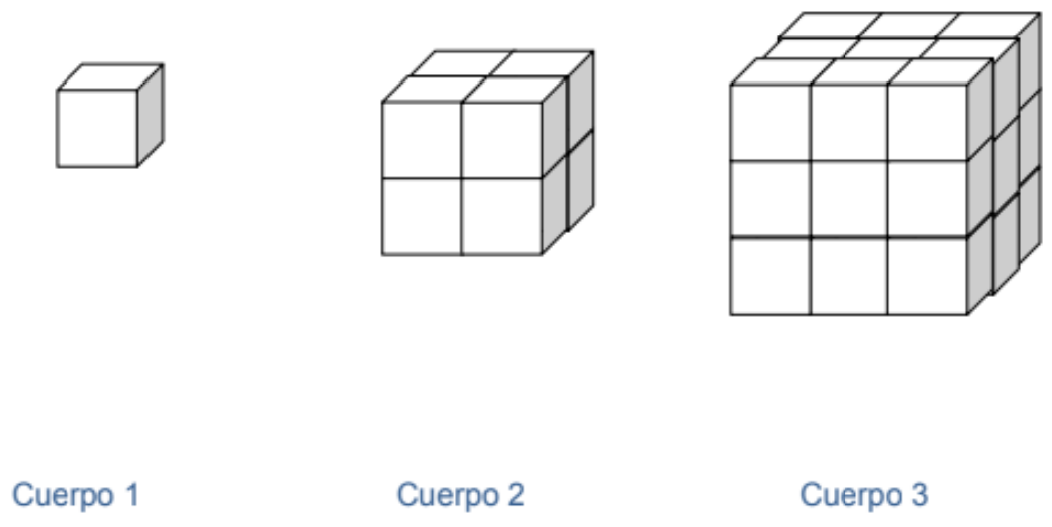
\includegraphics[width=0.7\linewidth]{Trabajos/04/Anexos/grafico_01.png}
		\caption{}
		\label{fig:grafico01}
	\end{figure}
\end{center}

\subsubsection{Terceras hora y media sincrónicas}

\begin{enumerate}
	\item Se retomará la actividad entre clases y se analizará cómo puede llevarse a cabo la gestión de la clase
	\item Se conformarán grupos para que cada uno resuelva una de las cinco actividades diseñadas en el documento “Matemática para la Formación	Docente” (\url{https://drive.google.com/file/d/1X_Hz86UvQZhWuBMkGTj9cY0JmMQt4Ia0/view?usp=sharing}) propuesto por Dirección de Educación Superior de la Provincia de Córdoba de la modelización con enfoque en la TAD.
	\item Puesta en común
	\item Recomendaciones finales por parte de los talleristas para trabajar el álgebra inicial a través de la modelización.
\end{enumerate}

\subsubsection{Evaluación final}

\begin{enumerate}
	\item  Se les proporcionará una actividad de modelización cuyo contenido principal será del álgebra inicial.
	\begin{enumerate}[{1}.1]
		\item Resuelva la actividad.
		\item Identifique el contexto de la situación planteada.
		\item Identifique los contenidos involucrados y el o los que se quiere enseñar.
		\item Justifique con marco teórico por qué corresponde a una actividad de modelación
		\item Exprese cómo gestionaría la clase
	\end{enumerate}
	
	\item En no menos de 4 líneas exprese una reflexión escrita sobre la experiencia del taller y el aprendizaje obtenido.
\end{enumerate}

\subsection{Bibliografía}

\nocite{*}
\printbibliography[keyword={04}]
	\clearpage
	%-------------------------------------------------------------------------
% INFORMACIÓN DEL ARTÍCULO
\thispagestyle{portadapage}
\setcounter{subsection}{0}
\setcounter{subsubsection}{0}
\setcounter{actividad}{0}
\setcounter{actividad_previa}{0}
\setcounter{actividad_entre}{0}
\renewcommand{\articulotipo}{Taller}
\renewcommand{\articulotitulo}{Avanzando con las propiedades de los conjuntos numéricos: Encadenamientos y ausencias entre la escuela Primaria y la escuela Secundaria}
\renewcommand{\articulotitulocorto}{Avanzando con las propiedades de los conjuntos numéricos}
\section{\articulotitulo}
\desctotoc{Villagra, C.; Carrasco, R.; Alvarez, D.; Miguez, I.}

\noindent\rule{\linewidth}{2pt}

\vspace{0.25cm}

\begin{flushright}
	\addautor[susannedaher013@gmail.com]{Mariette Susanne Daher}{Universidad Nacional de Salta}
	\vspace{1em}
	\addautor[]{Josefina Lávaque Fuente}{Universidad Nacional de Salta}
	\vspace{1em}
	\addautor[]{Blanca Azucena Formeliano}{Universidad Nacional de Salta}
\end{flushright}

\vspace{0.5cm}

\begin{center}
	\begin{minipage}{0.75\linewidth} \small
		\textsc{Resumen}. ~
		El taller tiene como intención promover las problemáticas de prácticas de enseñanza sobre el estudio de las propiedades de los conjuntos numéricos naturales $\mathbb{N}$; enteros $\mathbb{Z}$ y racionales $\mathbb{Q}$.
		
		Asimismo, se brindará entradas para el objeto de estudio con distintos caminos; que el docente podrá analizar y reformular teniendo en cuenta las continuidades y rupturas entre la escuela primaria y la escuela secundaria sobre las propiedades de los conjuntos numéricos.
		
		Desde la mirada didáctica que sostienen los documentos curriculares tanto nacionales como jurisdiccionales, se pretende problematizar los recorridos de los contenidos y prácticas propios de la escuela primaria y de la escuela secundaria sobre los conjuntos numéricos.
		
		Durante el taller se propondrán actividades que permitan estudiar y rescatar propiedades de los conjuntos numéricos que se estudian en la escuela primaria como uno más que, uno menos que, entre números naturales, regularidades en la serie escrita del conjunto de números naturales y se continuará con el estudio de las propiedades de los números enteros y racionales para reflexionar acerca de la continuidad y provisoriedad de los conocimientos construidos sobre las propiedades de los números naturales al ampliar cada conjunto numérico.
	\end{minipage}\\
\end{center}
%-------------------------------------------------------------------------

\subsection{Introducción}

Este taller contribuirá a profundizar las propiedades que poseen los conjuntos numéricos; las que son propias y las que se van incrementando a medida que se avanza en el estudio de los conjuntos numéricos; como así también permitirán el estudio y la reflexión alrededor de los obstáculos y los errores que se producen. Desde un punto de vista matemático y didáctico, por medio de la resolución de problemas, se propone reflexionar a través de:
\begin{itemize}
	\item Presentación y resolución de problemas.
	\item Socialización de los procedimientos que hacen a la resolución de problemas
	\item Elaboración de conclusiones, mediante diagramas o tablas
\end{itemize}

\subsection{Contenidos}

\begin{itemize}
	\item \textbf{Módulo 1}: Números naturales. Tabla numérica. Propiedades
	\item \textbf{Módulo 2}: Números enteros. Tabla numérica. La recta numérica. Propiedades.
	\item \textbf{Módulo 3}: Números racionales. La recta numérica. Propiedades
\end{itemize}

\subsection{Requisitos previos}

Los docentes deberán tener conocimiento sobre los NAP. Diseños Curriculares de primaria y secundaria.

\subsection{Objetivos}

\begin{itemize}
	\item Analizar las propiedades de los conjuntos numéricos en la resolución de problemas.
	\item Establecer las variables didácticas que permiten poner juego las propiedades de los conjuntos numéricos.
	\item Identificar problemas y estrategias de resolución en relación con las propiedades de los conjuntos numéricos en la propia tarea y de la tarea con otros colegas.
	\item Reflexionar acerca de las continuidades y rupturas entre la escuela primaria y la escuela secundaria sobre las propiedades de los conjuntos numéricos desde perspectivas de enseñanza de la matemática sostenidas en documentos curriculares.
\end{itemize}

\subsection{Actividades}

\subsubsection{Actividades previas}

Lectura y análisis del siguiente texto para comentar en la primera clase sincrónica.

\bigskip

\begin{center}
	\begin{minipage}{0.8\linewidth}
		\begin{center}
			\bfseries
			Números Naturales y Enteros
		\end{center}
		
		Los números naturales, de símbolo $\mathbb{N}$, son todos los números enteros positivos, es decir, todas aquellas cifras sin decimales y mayores a 0. Algunos ejemplos de números naturales son 1, 6, 23, 147 y 30500.
		
		Dependiendo del área de ciencia y el convenio utilizado, los números naturales se representan en uno de los siguientes conjuntos:
		\begin{itemize}
			\item El conjunto de naturales sin el cero, que comienza con 1: $\mathbb{N} = \{ 1, 2, 3, 4, 5, 6, 7, 8, \dots \}$
			\item El conjunto de naturales con el cero, que empieza con dicha cifra: $\mathbb{N} = \{ 0, 1, 2, 3, 4, 5, 6, 7, 8, \dots \}$
		\end{itemize}
		
		No obstante, como el 0 no puede ser ni positivo ni negativo, es preferible no incluirlo dentro del conjunto de números naturales, pues solo aborda los números enteros positivos.
		
		Los números naturales fueron los primeros números que empleamos para cuantificar objetos. Con el tiempo, los hemos utilizado para ordenar valores, comparar cantidades diferentes y como base para todo tipo de operaciones matemáticas. De hecho, para obtener otros números, como los fraccionarios, nos servimos muchas veces de los números naturales.
	\end{minipage}
	
		\bigskip
		
		\begin{minipage}{0.8\linewidth}
			\begin{center}
				\bfseries
				Propiedades de los números naturales
			\end{center}
			
			\textbf{Los números naturales solo presentan números enteros positivos, es decir, del 1 en adelante}. Los números negativos quedan fuera del conjunto de los naturales.
			
			\begin{itemize}
				\item Los números fraccionarios o con cifras decimales tampoco encajan en el conjunto de números naturales.
				\item Todos los números naturales poseen un sucesor y siguen un orden específico. En otras palabras, para cada número natural existe uno mayor que viene justo después ($4\to5$, $19\to20$, $110\to111$, $3041\to3042$, etc.).
				\item Hay una cantidad infinita de números naturales, ya que siempre podemos hallar un número natural que sea mayor a otro.
				\item Entre dos números naturales hay un número finito de naturales. Por ejemplo, entre 5 y 12 solo hay seis números naturales: 6, 7, 8, 9, 10 y 11.
			\end{itemize}
		\end{minipage}
		
		\bigskip
		
		\begin{minipage}{0.8\linewidth}
		\begin{center}
			\bfseries
			Clasificación y ejemplos de números enteros
		\end{center}
		
		Los números enteros se agrupan en tres subconjuntos: el 0, los enteros positivos y los enteros negativos. El 0 tiene su propia categoría al ser un \textbf{valor neutro}, es decir, un número que \textbf{no puede ser ni positivo ni negativo}.
		
		A continuación, compartimos propiedades y características de los números enteros:
		\begin{itemize}
			\item Existe una \textbf{cantidad infinita de números enteros}, tanto positivos como negativos. La prueba es que siempre podemos hallar un número entero más pequeño o más grande que otro número entero.
			\item \textbf{Entre dos números enteros} hay una \textbf{cantidad finita de enteros}. Por ejemplo, entre -7 y 4 existen 10 números enteros, que son: -6, -5, -4, -3, -2, -1, 0, 1, 2 y 3.
			\item Para cada número entero siempre hay otro mayor denominado \textbf{sucesor}. Por ello, los números enteros siguen un orden específico que no cambia. Por ejemplo, al número 5 le sigue el número 6, después del 101 viene el 102, y el sucesor de -21 es -20.
			\item En la recta numérica, \textbf{los números enteros más pequeños se sitúan a la izquierda}, mientras que \textbf{los más grandes se sitúan a la derecha}.
			\item Cualquier suma, resta y multiplicación entre dos números enteros siempre devolverá otro número entero. No es así con las divisiones, ya que hay casos en que la división de dos números enteros devuelve un número fraccionario, es decir, un valor con cifras decimales.
			\item El valor absoluto de un número entero es siempre el mismo, independientemente de su signo, ya que simplemente mide la distancia del número respecto al cero. Por ejemplo, el valor absoluto de $|+11|$ y $|-11|$ es igual: 11.
		\end{itemize}
	\end{minipage}
\end{center}

\bigskip

\subsubsection{Presentación del taller}

\begin{itemize}
	\item Objetivos, Contenidos, forma de trabajo
	\item Criterios e indicadores de evaluación.
	\item Trabajo grupal del problema 1
	\item Puesta en común
	\item Contenidos: Números naturales. Importancia de la tabla numérica. Propiedades de los números naturales
\end{itemize}

\begin{itemize}
	\item \textbf{Tareas grupales para exponer:}
	\begin{enumerate}
		\item Resuelva los siguientes problemas.
		\item Enuncie otro problema más complejo.
		\item Identifique los conceptos involucrados como saberes previos.
		\item NAP o Diseño Curricular Jurisdiccional de su provincia ¿Cuáles son los contenidos de la educación obligatoria propuestos en los diseños curriculares, que se relacionan con los problemas?
		\item Escriba un problema que se corresponda con 6to, 7mo, 8vo, 9no año de escolaridad obligatoria
	\end{enumerate}
	
	\item \textbf{Recursos:} Tabla numérica de los 100 primeros números naturales. Recta numérica. Recta numérica con números del -10 al 10
	
	\begin{actividad}
		~
		\begin{enumerate}[a.]
			\item Escribir el siguiente y el anterior de 49.
			\item Escribir el anterior de 1.
			\item Escribir todos los números comprendidos entre 63 y 89.
			\item ¿Es posible encontrar números naturales entre 39 y 40?
			\item ¿Cuánto es 1 más 1000? ¿y uno más 2000?
			\item Elegir un número de la tabla y escribir: Todos los números que están en la misma columna y en la misma fila. ¿Qué observa de la secuencia de números escritos?
			\item ¿Qué propiedades están implícitas en las consignas anteriores? Identificarlas y escribirlas en forma coloquial y simbólica.
			\item ¿En qué se diferencia utilizar la tabla o la recta numérica?
			\item ¿Qué potencial se observa en la recta numérica para destacar las propiedades recién
			vistas?
		\end{enumerate}
	\end{actividad}
\end{itemize}

\subsubsection{Clase asincrónica}

\begin{itemize}
	\item \textbf{Tiempo:} 3 hs
\end{itemize}

\begin{actividad}
	~
	\begin{enumerate}[a.]
		\item Elaborar un relato de fortalezas y debilidades del primer encuentro sincrónico.
		\item Construir la tabla numérica de los 100 primeros números enteros negativos
	\end{enumerate}
\end{actividad}

\subsubsection{Clase sincrónica 2}

\begin{itemize}
	\item \textbf{Tiempo:} 1 $\nicefrac12$ hs
	
	\item \textbf{Contenidos:} Propiedades de los números enteros
	
	\item \textbf{Recursos:} Tabla numérica de los 100 primeros números naturales. Recta numérica. Tabla numérica de los 100 primeros números enteros negativos. Recta numérica con números del -10 al 10
	
	\item \textbf{Tareas grupales para exponer:}
	\begin{enumerate}[a.]
		\item Resuelva los siguientes problemas en grupo.
		\item Enuncie otro problema más complejo.
		\item Identifique los conceptos involucrados como saberes previos.
		\item NAP o Diseño Curricular Jurisdiccional de su provincia ¿Cuáles son los contenidos de la educación obligatoria propuestos en los diseños curriculares, que se relacionan con los problemas?
		\item Escriba un problema que se corresponda con el 6to, 7mo, 8vo, 9no año de escolaridad obligatoria
	\end{enumerate}
\end{itemize}

\begin{actividad}
	~
	\begin{enumerate}[a.]
		\item Con la tabla de los 100 primeros números negativos.
		\item ¿Se podrán enunciar las mismas tareas que las efectuadas en Actividad 1? Si la respuesta es negativa: ¿Qué cambia?
		\item ¿Qué propiedades están implícitas en las consignas anteriores? Identificarlas y escribirlas en forma coloquial y simbólica
		\item ¿En qué se diferencia utilizar la tabla o la recta numérica para el estudio de los números enteros?
		\item ¿Qué potencial se observa en la recta numérica para destacar las propiedades recién vistas?
	\end{enumerate}
\end{actividad}

\subsubsection{Clase asincrónica}

\begin{itemize}
	\item \textbf{Tiempo:} 3 hs
\end{itemize}

\begin{actividad}
	~
	\begin{enumerate}[a.]
		\item Elaborar un relato de fortalezas y debilidades el segundo encuentro sincrónico
		\item Analizar los siguientes videos e identificar las propiedades de los números fraccionarios que enseña la docente.
		
		\url{https://youtu.be/MPAuLf8C8IE?si=8n6DSfR4qtZ3ZjAn}
		
		\url{https://youtube.com/watch?v=uopbujGp5X8&feature=shared}
		
		\item A partir del análisis de tareas en los libros de texto formular cinco tareas, en los años que se desempeña a partir de las cuales se deduzcan algunas de las propiedades de los números enteros.
		
		A continuación, se presentarán las propiedades las propiedades del sistema de numeración y de los conjuntos numéricos de naturales, enteros y racionales.
	\end{enumerate}
\end{actividad}

\subsubsection{Clase sincrónica 3}

\begin{itemize}
	\item \textbf{Tiempo:} 1 $\nicefrac12$
	\item \textbf{Contenidos:} Números racionales y la recta numérica. Completitud en $\mathbb{R}$. Evaluación.
	\item \textbf{Recursos:} Tabla numérica de los 100 primeros números naturales. Recta numérica. Tabla numérica de los 100 primeros números enteros negativos. Recta numérica con números del -10 al 10.
\end{itemize}

\begin{actividad}
	~
	\begin{enumerate}
		\item Qué recurso utilizarías o sería más adecuado para deducir las propiedades de los números racionales?
		\item ¿Cuáles son esas propiedades? Justificar.
		\item ¿Se podrán enunciar las mismas tareas que las efectuadas en la Actividad 2? Si la respuesta es negativa: ¿Qué cambia?
	\end{enumerate}
\end{actividad}

\subsubsection{Evaluación}

\begin{enumerate}
	\item A partir del análisis de tareas en los libros de texto formular cinco tareas, a partir de las cuales se deduzcan algunas de las propiedades de los números RACIONALES.
	\item Elaborar un relato de fortalezas y debilidades del taller. Enviar hasta el 10 de agosto.
\end{enumerate}

\subsection{Bibliografía}

\nocite{*}
\printbibliography[keyword={05}]
	\clearpage
	%-------------------------------------------------------------------------
% INFORMACIÓN DEL ARTÍCULO
\thispagestyle{portadapage}
\setcounter{subsection}{0}
\setcounter{subsubsection}{0}
\setcounter{actividad}{0}
\setcounter{actividad_previa}{0}
\setcounter{actividad_entre}{0}
\renewcommand{\articulotipo}{Comunicación breve}
\renewcommand{\articulotitulo}{Redefiniendo el sentido de las fracciones: Aportes para su enseñanza desde la Teoría de Representaciones Semióticas y el Juego de Marcos}
\renewcommand{\articulotitulocorto}{Redefiniendo el sentido de las fracciones}
\section{\articulotitulo}
\desctotoc{Villagra, C.; Carrasco, R.; Alvarez, D.; Miguez, I.}

\noindent\rule{\linewidth}{2pt}

\vspace{0.25cm}

\begin{flushright}
	\addautor[celinaansaldi18@hotmail.com]{Maria Celina Ansaldi}{-}
	\vspace{1em}
	\addautor[]{Lucrecia Silvina Ponce}{-}
	\vspace{1em}
	\addautor[]{Francisco Javier Azar}{-}
\end{flushright}

\vspace{0.5cm}

\begin{center}
	\begin{minipage}{0.75\linewidth} \small
		\textsc{Resumen}. ~
		Este taller se propone mejorar la enseñanza de las fracciones, un concepto fundamental y a su vez complejo debido a las tensiones existentes sobre su enseñanza en el nivel primario y secundario. El contenido se abordará mediante la resignificación de estrategias de enseñanza basadas en la relación parte-todo como generadoras de lenguaje y símbolos, fundamentadas en la Teoría de las Representaciones Semióticas de Raymond Duval y el juego de Marcos de Régine Douady. A través de esta aproximación, se procura recuperar las potencialidades del uso y creación de material didáctico aplicable a la enseñanza de las fracciones. En la propuesta se plantean situaciones problemáticas donde los conceptos emergen como  facilitadores de resoluciones, mediante  representaciones, manipulación de material concreto e interpretaciones. Esta mirada integrada facilita una comprensión profunda y significativa de las fracciones, promoviendo reflexiones sobre las prácticas docentes y fomentando un aprendizaje conceptual sólido y significativo.
	\end{minipage}
\end{center}
%-------------------------------------------------------------------------

\subsection{Introducción}

La comprensión significativa de los conceptos matemáticos en los estudiantes es un objetivo fundamental en los niveles primario y secundario. Sin embargo, la enseñanza de las fracciones presenta desafíos debido a su naturaleza abstracta y a las dificultades que los estudiantes encuentran para entender su utilidad y sentido. Estas dificultades nos obligan a cuestionar y reevaluar nuestras propias prácticas educativas: ¿Cómo pueden los estudiantes utilizar fracciones si no las comprenden plenamente? ¿En qué nivel deberían enseñarse y cómo podemos asegurarnos que su enseñanza sea efectiva?

Hans Freaudenthal (1980) observó que las fracciones y las operaciones con ellas, a menudo consideradas complejas, son construcciones que solo se comprenden adecuadamente en niveles superiores. Si bien su estudio se inicia en el nivel primario y continúa en el nivel secundario, el tiempo de permanencia en estos trayectos escolares no suele asegurar una comprensión significativa, sino limitada. En este sentido, la investigación de Mack (1990) sugiere que muchos estudiantes tienen una comprensión limitada de fracciones como números y como parte del conjunto de números racionales que las contienen, a menudo luchan con su interpretación y los procedimientos algorítmicos que han aprendido. Si miramos el contexto universitario, los alumnos tienden a colocar estas complicadas operaciones en sus calculadoras científicas, otorgándole un uso instrumental para resolver distintas situaciones de la disciplina o ciencia que estudian. Este contexto tecnológico debería implicar una disminución de tiempo al trabajo algorítmico, especialmente de expresiones complejas, empleándolo en profundizar en los conceptos, incluir temas no considerados y en desarrollar destrezas de un nivel cognitivo más alto, como el cálculo aproximado, la estimación, etc. (Linares, S \& Sánchez, M; 2009).

Aunque este taller no se centra en el uso de tecnologías, reconocemos su potencial para el aprendizaje matemático. Sin embargo, hemos optado por el uso y elaboración de material didáctico tangible como una forma de redefinir el aprendizaje de fracciones de una manera concreta y accesible, y como elemento de transición de la enseñanza de fracciones entre el nivel primario y secundario.

Se pretende abordar estos desafíos utilizando un enfoque teórico con los aportes de Raymond Duval para las \textbf{representaciones} del concepto de Fracción y los de Regine Duady con el Juego de Marcos, que da lugar a las distintas \textbf{interpretaciones} con las que trabajaremos. Desde un enfoque práctico se favorecerá a los asistentes al taller con distintas situaciones que involucren el uso de material didáctico como punto de partida para el desarrollo del lenguaje de fracciones, otorgando de significado a los símbolos que representan al concepto y permitan interpretarlo. La relación Parte-Todo, puede entenderse como el origen de otras interpretaciones de las Fracciones, siendo de las más intuitivas para el niño o adolescente y como generadora de lenguaje, contribuirá a las posteriores interpretaciones del concepto.

Es esencial entender que la práctica pedagógica va más allá de enseñar algoritmos y conceptos matemáticos, debemos reflexionar sobre el ``\textit{por qué}'' y el ``\textit{para qué}'' que existe detrás del hacer matemáticas, para interpretar el proceso de construcción del conocimiento matemático de los estudiantes, los obstáculos que enfrentan y cómo abordarlos de manera efectiva diseñando distintas estrategias.

Por último y no menos importante, se busca reflexionar sobre la propia práctica docente, identificando áreas de mejora y fortalecimiento en cuanto a la enseñanza de fracciones. Este trabajo metacognitivo estará presente en el recorrido de este taller a través de cuestionamientos guiados, permitiendo a los asistentes tomar conciencia de sus propias creencias, apropiarse de ideas sobre el proceso de enseñanza-aprendizaje del concepto de fracción, debatir y compartir opiniones con otros, ampliando sus perspectivas, comunicando sus conclusiones y porque no, aplicando esta práctica en el aula.

De lograrlo, nuestro trabajo estará hecho.

\subsection{Contenidos}

\begin{itemize}
	\item \textbf{Módulo 1: Fundamentos y Teorías}
	\begin{itemize}
		\item \textit{Introducción al taller}: La fracción como parte de un todo y parte de una parte. La fracción como medida y en Contexto continúo.
		\item \textit{Teorías y enfoques pedagógicos}: Juego de Marcos de Regine Douady. Representaciones semióticas de Raymond Duval.
	\end{itemize}
	
	\item \textbf{Módulo 2: Conceptos a integrar}
	\begin{itemize}
		\item La fracción como una razón.
		\item Operaciones con fracciones dentro del Campo Aditivo y Multiplicativo. Representaciones.
	\end{itemize}
	
	\item \textbf{Módulo 3: Tipos de fracciones.}
	\begin{itemize}
		\item \textit{Clasificación}: Fracciones propias, impropias, aparentes y mixtas.
		\item \textit{Relaciones entre fracciones}: Fracciones equivalentes y sus aplicaciones como punto integrante de integración y aplicación.
	\end{itemize}
\end{itemize}

\subsection{Requisitos previos}

\begin{enumerate}[3.1-]
	\item \textit{Nivel educativo:} Dirigido a docentes de niveles primario y secundario. Estudiantes avanzados de la carrera del Profesorado de Nivel Primario y del profesorado de educación secundaria en matemática.
	\item \textit{Conocimiento y experiencia:} Familiaridad con conceptos relacionados con fracciones. Experiencia previa en la enseñanza o estudio de matemáticas y su didáctica en niveles primario y secundario.
	\item \textit{Herramientas y recursos:} Disponibilidad de una computadora con conexión a internet estable. Instalación previa de la aplicación ZOOM para participar de los encuentros sincrónicos. Nociones básicas de la dinámica virtual en plataformas como Moodle.
	\item \textit{Actitud y compromiso:} Hacemos referencia al interés por reflexionar sobre prácticas pedagógicas actuales y disposición para explorar nuevas estrategias didácticas. Participación activa y colaborativa con otros docentes y/o estudiantes.
\end{enumerate}

\subsection{Objetivos}

\begin{itemize}
	\item Desarrollar una comprensión significativa de las Fracciones, facilitando estrategias y herramientas didácticas.
	\item Integrar teorías educativas utilizando las representaciones semióticas y el juego de marcos que generen distintas interpretaciones en la enseñanza de fracciones.
	\item Instruir en el uso de material didáctico tangible capacitando a los asistentes en su elaboración facilitando un aprendizaje concreto y significativo.
	\item Fomentar la mejora de la práctica docente a través de espacios de reflexión metacognitiva y el intercambio de experiencias que promuevan un análisis colectivo y colaborativo.
\end{itemize}

\subsection{Actividades}

\subsubsection{Actividades previas}

En la plataforma de soporte del curso, se comunicarán a los participantes los objetivos del taller y estarán disponibles los materiales a imprimir para el primer encuentro sincrónico y dos materiales de lectura recomendada. El primer documento, de creación propia, abordará los contenidos teóricos seleccionados que sustentan este taller, incluyendo la Teoría del Juego de Marcos de Régine Douady y la Teoría de las Representaciones de Raymond Duval. El segundo documento, titulado “Los significados de las fracciones: una perspectiva fenomenológica”, explorará los diferentes sentidos e interpretaciones de las fracciones que se discutirán durante los encuentros sincrónicos.

Los participantes deberán descargar y leer estos materiales, ya que serán fundamentales para las actividades del primer encuentro sincrónico. Además, se les anima a reflexionar y responder las siguientes preguntas, las cuales servirán como punto de partida para iniciar el taller:

\bigskip
\begin{center}
	\begin{minipage}{0.8\linewidth}
		\itshape
		\begin{enumerate}[1.]
			\item ¿Desde sus prácticas docentes o experiencia como estudiantes residentes, qué desafíos enfrentan al enseñar fracciones? ¿Cómo los abordan?
			\item ¿Qué estrategias han encontrado más efectivas para enseñar fracciones en el aula?
			\item ¿Podrían establecer diferencias en la comprensión de fracciones entre estudiantes de primaria y secundaria? ¿Cómo han adaptado su enseñanza a estos diferentes niveles educativos?
		\end{enumerate}
	\end{minipage}
\end{center}
\bigskip

Durante el primer encuentro sincrónico, se tomarán algunos minutos en los que se revisarán y debatirán las respuestas a estas preguntas, promoviendo un análisis colectivo antes de iniciar plenamente el taller.

\subsubsection{Primera hora y media sincrónica}

\begin{enumerate}
	\item Para iniciar el taller, comenzaremos con una breve presentación de los autores, se expondrán los objetivos generales y se ofrecerá un panorama general de las actividades planificadas.
	
	Se dedicará un momento a recuperar las respuestas de la actividad previa facilitando un análisis colectivo. Utilizaremos una presentación en PowerPoint para introducir conceptos claves necesarios para el desarrollo del taller, basándonos en los principios de las representaciones semióticas de Duval, que enfatizan la importancia de múltiples representaciones para comprender los conceptos matemáticos.
	
	\item \textbf{Construcción del Muro de Fracciones mediante el plegado de papel}: Los	participantes tendrán la oportunidad de construir el material didáctico denominado ``Muro de Fracciones'' utilizando el material descargado previamente desde la plataforma. Este ejercicio práctico permitirá explorar visualmente los conceptos de fracción como \textit{Parte de un Todo}, haciendo uso de las representaciones concretas recomendadas por Duval ya que el plegado de papel facilita la diversificación de las mismas.
	
	\begin{figure}
		\centering
		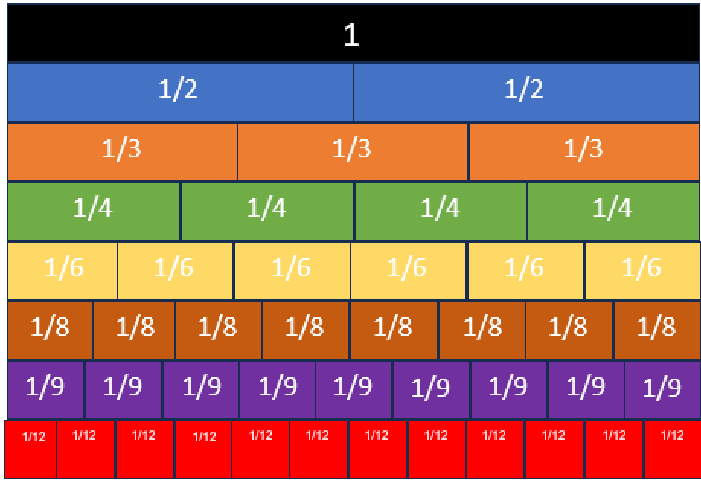
\includegraphics[width=0.6\linewidth]{Trabajos/06/Anexos/grafico_01}
		\caption{Fuente: elaboración propia}
		\label{fig:grafico_06_01}
	\end{figure}
	
	\item \textbf{Preguntas de reflexión durante la actividad:} \textit{¿Es posible plegar una tira de papel en 5 partes iguales? ¿Y en 7 partes iguales?} Estos interrogantes se plantean como propuestas de investigación para explorar más a fondo en sesiones posteriores, siguiendo el enfoque de investigación propuesto por Douady en el Juego de Marcos, que promueve la exploración y la experimentación como parte integral del aprendizaje matemático, por lo que se espera que los participantes a partir de esta experiencia, deduzcan la necesidad de un cambio de marco para dicha construcción, el geométrico.
	
	\item \textbf{Actividad grupal:} Una vez construido el Muro de Fracciones, los participantes se dividirán en \textbf{grupos} para reflexionar sobre la elaboración del material y las relaciones que emergen de él, tanto en términos de la totalidad como de las partes que lo componen, profundizando así en el significado de la fracción desde la perspectiva de las representaciones semióticas, analizando como diferentes representaciones pueden facilitar una comprensión más profunda del concepto de fracción.
	
	\item \textbf{Análisis comparativo:} También se les invita a analizar qué propiedades de los números naturales son aplicables y cuáles requieren ajustes en el contexto de las fracciones, apoyándose en las teorías de Duval y Duady para entender cómo las representaciones y marcos mentales influyen en la comprensión matemática.
	
	\item \textbf{Cierre:} Al concluir este primer encuentro sincrónico, se compartirá un Power Point con las ideas principales de las teorías de Duval y Doaudy que refuercen las lecturas sugeridas en la actividad previa.
	
	Utilizando el material creado, se les propondrá a los participantes crear un nuevo ``Muro de Fracciones'' que incluya las \textbf{fracciones equivalentes} encontradas durante la actividad, fomentando la aplicación práctica de los conceptos explorados.
\end{enumerate}

\subsubsection{Primeras tres horas entre clases}

\begin{enumerate}
	\item Se les solicitará que entreguen en la plataforma la resolución de la actividad:
	
	\begin{quote}
		\textit{Analicen y documenten utilizando el material Muro de Fracciones 3 formas diferentes de representar y obtener el entero. ¿Cómo estas representaciones pueden ser interpretadas por sus estudiantes? (primario-secundario)} Se sugiere subir un archivo Word en el que inserten imágenes de los muros que proponen con sus respectivas aclaraciones.
	\end{quote}
	
	\item Preguntas reflexivas: “\textit{¿Qué dudas u obstáculos podrían surgir entre sus estudiantes al realizar actividades con el muro de fracciones? ¿Cómo podrían abordarse estas dudas desde las teorías de Duval y Doaudy?}”
	
	\item Se compartirá un documento colaborativo en formato Drive, en el que los participantes harán breves intervenciones escritas destacando los hallazgos y análisis realizados. En él deberán considerar cómo estos podrían influir en su práctica docente y en la comprensión de sus estudiantes. De esta manera, se busca consolidar el aprendizaje desde los fundamentos teóricos y prácticos proporcionados por los organizadores del taller.
\end{enumerate}

\subsubsection{Segundas hora y media sincrónicas}

\begin{enumerate}
	\item Utilizaremos una presentación de Power Point para retroalimentar la corrección de la actividad entregada en el campus destacando cómo se puede validar la solución del plegado en 5 y 7 partes, a partir de los conceptos y métodos discutidos en el primer encuentro sincrónico.
	\item Continuaremos con la presentación para introducir el concepto de fracción como razón y su aplicación en la ubicación de números fraccionarios en la recta numérica utilizando el plegado de papel para ilustrar el concepto de manera visual y tangible.
	\item Procederemos a dividir a los talleristas en grupos y les asignaremos a cada grupo una actividad diferente, ordenarán fracciones en la recta utilizando como recurso el plegado de papel, un recurso privilegiado que colabora para que el alumno trabaje utilizando dicho sentido y no se presenten los obstáculos cognitivos de la representación en la recta utilizando procedimientos aritméticos.
	
	Se les propondrá entonces la resolución de actividades extraídas de:
	\begin{itemize}
		\item Itzcovich, Horacio. El Abecé de La Matemática Escolar. Capítulo 5: El trabajo escolar en torno a las fracciones, página 150.
		\item Documento curricular: Matemática: Fracciones y Números Decimales. Apuntes para la enseñanza. 6to grado. (2005). Gobierno de la Ciudad de Buenos Aires. Secretaría de Educación, página 17.
		\item Documento curricular: Matemática: Fracciones y Números Decimales. Apuntes para la enseñanza. 5to grado. (2005). Gobierno de la Ciudad de Buenos Aires. Secretaría de Educación, páginas 25, 26 y 27.
	\end{itemize}
	
	Luego, les propondremos reflexionar sobre las siguientes cuestiones:
	\begin{itemize}
		\itshape
		\item “¿Cuáles son los argumentos que un alumno, al finalizar 6to/7mo grado y de 1er año de secundaria estaría en condiciones de elaborar cuando resuelve este tipo de problemas?”,
		\item “¿Cómo crees que podría beneficiar en tus prácticas esta metodología de trabajo?”,
		\item “¿Qué fortalezas y debilidades puedes identificar en las resoluciones utilizando el plegado de papel?”
	\end{itemize}
	
	\item Cierre: Finalizado el momento de socialización de las diferentes resoluciones retomaremos las preguntas de reflexión para cerrar la actividad, animando a los participantes a implementar estas estrategias en sus prácticas.
\end{enumerate}

\subsubsection{Segundas tres horas entre clases}

\begin{enumerate}
	\item Deberán entregar en la plataforma en un archivo de Word actividades en las cuales deberán \textbf{ubicar números fraccionarios y decimales en la recta numérica a partir del uso del plegado de papel}.
	
	Las actividades serán extraídas de:
	\begin{itemize}
		\item Documento curricular: Matemática: Fracciones y Números Decimales. Apuntes para la enseñanza. 5to grado. (2005). Gobierno de la Ciudad de Buenos Aires. Secretaría de Educación, páginas 25, 26 y 27.
		\item Seoane, Silvana. Matemática material para docentes sexto grado educación primaria 1a ed. - Ciudad Autónoma de Buenos Aires: Instituto Internacional de Planeamiento de la educación IIPE-Unesco, 2012, páginas: 33 y 43.
	\end{itemize}
	
	\item El juego del \textbf{Tangram} favorece el pensamiento matemático, es un antiguo rompecabezas chino compuesto por 7 piezas: un cuadrado, un paralelogramo romboide y 5 triángulos semejantes diferentes. Los alumnos deberán ingresar al siguiente link: \url{https://www.youtube.com/watch?v=7wWQWUWHr5U} para construir el Tangram a partir del plegado de papel, este rompecabezas será el insumo para el Tercer encuentro sincrónico.
\end{enumerate}

\subsubsection{Terceras hora y media sincrónicas}

\begin{enumerate}
	\item Daremos comienzo a este último encuentro sincrónico con una presentación de Power Point para retroalimentar la actividad entregada en la segunda hora entre clases.
	\item Continuaremos con la presentación para reconstruir el recorrido realizado en los distintos momentos del taller: encuentros sincrónicos y momentos de estudio y de resolución de actividades asincrónicas, destacando los conceptos y sentidos de las fracciones, cómo llevarlos a la práctica con el uso de material tangible y los aportes de las teorías en los que se apoya este taller.
	\item Dividiremos a los talleristas nuevamente en grupos y les propondremos trabajar con una última actividad para poder relacionar y recuperar todo lo visto y analizado hasta el momento: El Tangram.
	\item Los invitaremos a reflexionar sobre:
	\begin{itemize}
		\item cómo surge el sentido de la fracción Parte-Todo y Parte de una parte,
		\item cómo hallar la medida de cada pieza del Tangram,
		\item las diferentes formas de hallar una parte del Tangram a partir de otras partes del mismo,
		\item equivalencias de áreas de diferentes figuras,
		\item cómo reconstruir figuras más pequeñas con las partes del Tangram, cómo hallar el área de la misma y su validación,
		\item relaciones de orden,
		\item los contenidos que circulan en las actividades,
		\item los conocimientos previos de los alumnos.
	\end{itemize}
	\item Finalizado el momento de trabajo grupal intervendremos para proponer la socialización sobre el análisis y reflexión de la propuesta de trabajo con el Tangram, destacaremos cómo puede invitarnos a repensar nuestras prácticas o futuras prácticas el uso de material didáctico al momento de abordar la enseñanza de las fracciones en el nivel primario y ciclo básico del secundario para favorecer el aprendizaje significativo de los estudiantes.
	\item Cerraremos el taller con unas palabras de reflexión a modo de conclusión. También, se les explicará que para acreditar el taller deberán completar una instancia evaluativa disponible en la plataforma.
\end{enumerate}

\subsubsection{Evaluación final}

\begin{enumerate}
	\item Para evaluar nuestra propuesta de taller, dejaremos disponible en la plataforma una encuesta que permitirá a los participantes realizar su feedback sobre la experiencia.
	\item Además, solicitaremos la entrega de la siguiente actividad para acreditar su participación en el Taller: "Redefiniendo el Sentido de las Fracciones: Aportes para su Enseñanza desde la Teoría de Representaciones Semióticas y el Juego de Marcos".
\end{enumerate}

\bigskip
\begin{center}
	\begin{minipage}{0.8\linewidth}
		\textbf{Actividad evaluativa}
		
		Buscar en libros de texto escolares del segundo ciclo de Educación Primaria y/o Ciclo Básico de la Escuela Secundaria una actividad que permita abordar la enseñanza de las fracciones en el sentido de Parte-Todo o como una Razón. Luego, analizar la misma a partir de preguntas que los inviten
		a reflexionar:
		\begin{itemize}
			\item ¿Qué conocimientos previos y habilidades matemáticas deben poner en juego los alumnos? Explica cómo la actividad puede ayudar a desarrollar una comprensión significativa de fracciones.
			\item Diversidad de representaciones: La actividad elegida, ¿propone la utilización de diferentes marcos y representaciones en su resolución? Identifique y describa brevemente.
			\item Integración de estrategias didácticas: ¿Que modificaciones sugerirías, para incorporar las estrategias de enseñanza de las fracciones con material didáctico vistas durante el taller? Describa cómo estos cambios podrían mejorar la comprensión de los estudiantes.
			\item Impacto en la práctica docente: ¿Cómo crees que las sugerencias propuestas podrían enriquecer tus prácticas docentes? Reflexiona sobre los posibles beneficios y desafíos de implementar estos cambios. ¿Qué conocimientos ponen en juego los alumnos al resolver dicha actividad?
		\end{itemize}
	\end{minipage}
\end{center}
\bigskip

Los participantes entregarán en un archivo Word la actividad elegida y su análisis. En la plataforma se habilitará un espacio creado para tal fin. Tendrán un plazo máximo de una semana (sujeto a revisión) para completar y subir el archivo de manera individual o en pareja. La corrección y devolución de las evaluaciones tendrán lugar por medio de la plataforma, con un plazo máximo de una semana (tiempo sujeto a revisión por parte de la organización).

\subsection{Bibliografía}

\nocite{*}
\printbibliography[keyword={06}]
	\clearpage
	%-------------------------------------------------------------------------
% INFORMACIÓN DEL ARTÍCULO
\thispagestyle{portadapage}
\setcounter{subsection}{0}
\setcounter{subsubsection}{0}
\setcounter{actividad}{0}
\setcounter{actividad_previa}{0}
\setcounter{actividad_entre}{0}
\renewcommand{\articulotipo}{Comunicación breve}
\renewcommand{\articulotitulo}{Investigación sobre las estrategias de enseñanza implementadas en un profesorado de matemática durante la pandemia por COVID-19}
\phantomsection
\stepcounter{section}
\addcontentsline{toc}{section}{\protect\numberline{\thesection} \articulotitulo}
\desctotoc{Montenegro, F.; Cravero, M.; Fernández, C.; Salazar, M. G. R.}

\begin{center}
	\setstretch{1.5}
	{\Huge \scshape 
		\articulotitulo
	}
\end{center}

\noindent\rule{\linewidth}{2pt}

\vspace{0.25cm}

\begin{flushright}
	{\Large \scshape
		Fabiana Montenegro
	}\\
	{\large \itshape
		Escuela Normal Superior N° 32 “General José de San Martín”
	}\\
	{\ttfamily \small
		montenegrofg@gmail.com
	}\\ \vspace{1em}
	{\Large \scshape
		Mariela Cravero
	}\\
	{\large \itshape
		Escuela Normal Superior N° 32 “General José de San Martín”
	}\\ \vspace{1em}
	{\Large \scshape
		Carlos Fernández
	}\\
	{\large \itshape
		Escuela Normal Superior N° 32 “General José de San Martín”
	}\\ \vspace{1em}
	{\Large \scshape
		María Gracia Raquel Salazar
	}\\
	{\large \itshape
		Escuela Normal Superior N° 32 “General José de San Martín”
	}\\
\end{flushright}

\vspace{0.5cm}

\begin{center}
	\begin{minipage}{0.75\linewidth} \small
		\textsc{Resumen}. ~
		Con el objeto de promover la función de investigación y suscitar la producción de conocimiento educativo y pedagógico en el nivel Superior y en los Institutos Superiores de Formación Docente (ISFD) el Instituto Nacional de Formación Docente (INFoD) en el año 2021 convocó a las y los docentes y estudiantes de carreras de Formación Docente de Institutos Superiores de gestión estatal a presentar proyectos de investigación. El eje priorizado, en dicha convocatoria, fue la educación en Argentina en el contexto de la emergencia sanitaria generada por el Coronavirus SARS-CoV-2. En el marco de dicha convocatoria los autores de esta ponencia presentamos un proyecto cuyo objetivo fue indagar y analizar, desde lo didáctico y lo curricular, las estrategias de enseñanza implementadas por las y los docentes de los espacios curriculares de la formación específica y de la formación en la práctica profesional del Profesorado de Educación Secundaria en Matemática del ISFD N°32 de Santa Fe, durante la pandemia por COVID-19. En este trabajo  presentamos los resultados de una encuesta que formó parte de la investigación desarrollada en el 2022.
	\end{minipage}
\end{center}
%-------------------------------------------------------------------------

\subsection{Introducción}

Esta ponencia describe algunos resultados derivados de una investigación referida a las estrategias de enseñanza llevadas a cabo en un profesorado de matemática para la educación secundaria durante los años de la pandemia. Consideramos que esta comunicación en las JEM favorece el intercambio de análisis de experiencias de un hecho reciente que obligó a todos los niveles del sistema educativo de 190 países del mundo a desarrollar tareas educativas en entornos virtuales.

\subsection{Requisitos previos}

Profesores y profesoras de Matemática y estudiantes de Profesorado de Matemática.

\subsection{Desarrollo}

Como consecuencia del Aislamiento Social Preventivo y Obligatorio (ASPO) el cuerpo docente se vio en la necesidad de adaptarse y brindar respuestas a las necesidades educativas de los y las estudiantes. Tal como otros educadores, llamamos a este escenario Educación Remota de Emergencia (ERE).

En este contexto, para desarrollar las propuestas educativas gran parte del colectivo docente recurrió al uso de TIC. Según \textcite{coll2011}, las propuestas educativas que incorporan las TIC con un cierto nivel de elaboración deberían incluir tres tipos de ingredientes: los recursos y software que profesores y alumnos utilizan para enseñar y aprender; un diseño instruccional elaborado y explícito con objetivos, contenidos y actividades de enseñanza, aprendizaje y evaluación y un conjunto de normas y sugerencias sobre cómo utilizar dichas herramientas. En síntesis, las propuestas educativas apoyadas en las TIC incluyen dos aspectos interdependientes: tecnológicos como pedagógicos, que se integran en lo que \textcite{coll2011} denominó un diseño tecnopedagógico.

Cabe aclarar que al hablar de TIC haremos referencia tanto a los dispositivos, aplicaciones, software informáticos como a las acciones que éstos habilitan para la enseñanza y el aprendizaje de la matemática. En cuanto a los usos que pueden darse a dichos recursos adoptamos la clasificación que se presenta en \textcite{bravo2016} diferenciando 2 dimensiones: los vinculados a la matemática (para producir matemática, para recibir información matemática, para comunicar información matemática) y los vinculados con la comunicación.

En relación al concepto de estrategias de enseñanza (EE), recuperamos la conceptualización de \textcite{anijovich2010} que define las EE como el conjunto de decisiones que asume el docente para orientar la enseñanza de un contenido disciplinar teniendo en cuenta qué quiere que los estudiantes comprendan, por qué y para qué.

Bajo este marco de referencia, consideramos indagar y analizar las EE implementadas por los y las docentes para desarrollar su propuesta educativa.

Considerando que la complejidad del objeto de estudio de esta investigación requería la utilización e integración de diferentes abordajes metodológicos, planteamos una investigación exploratoria y descriptiva y optamos por el enfoque metodológico conocido como método mixto, que complementa los métodos cualitativos y cuantitativos.

Para dar respuesta a nuestro problema de investigación, en primer lugar, se profundizó el marco teórico. En segundo lugar, se llevó a cabo una encuesta online a través de formulario de Google a las y los profesores de manera voluntaria y anónima. Seguidamente, se realizaron entrevistas en profundidad a algunos de las y los docentes encuestados. Culminamos analizando materiales didácticos que nos compartieron algunos docentes de manera voluntaria y que se desarrollaron durante el ASPO.

Por cuestiones de espacio a continuación presentaremos el análisis de una pregunta que formó parte de la encuesta. Decidimos presentar, en este trabajo, los resultados parciales de la encuesta puesto que constituyó nuestro primer instrumento de recolección de datos, porque nos permitió aprovechar conceptos y gráficos variados de la estadística descriptiva y porque de ella surgieron hipótesis que buscamos ratificar o rectificar en las entrevistas.

En una de las preguntas se pedía vincular diferentes recursos tecnológicos con los usos que se les dieron para la enseñanza de la matemática. Las y los docentes encuestados debieron elegir entre los siguientes recursos: aula virtual del INFoD, videoconferencias, mensajería interna, aplicativos, presentación, buscadores y redes sociales. Y los posibles usos dados: para debatir, compartir información, buscar información, emplear en la ejercitación, producir materiales, aprender definiciones, propiedades, procedimientos, comunicarse con las/os estudiantes.

Luego de analizar los resultados de las encuestas y empleando gráficos estadísticos para su interpretación puede concluirse que, el debate se desarrolló durante la ERE en mayor medida a través del Aula virtual del INFoD (60\%) y de videoconferencias (70\%). Todos los recursos tecnológicos considerados fueron empleados en el debate con y entre los estudiantes. Los recursos mayormente empleados para compartir resolución de ejercicios fueron el Aula Virtual del INFoD (60\%), videoconferencias (55\%) y presentaciones (50\%). También fueron importantes los aplicativos (GeoGebra, Excel, etc.) (35\%). Para la búsqueda de información no se emplearon las redes sociales como se esperaba; sino que, fue mayormente a través de buscadores de la web (Google, Bing, etc.) (55\%) y del Aula Virtual del INFoD (50\%).

Los aplicativos fueron el recurso más utilizado en el empleo de ejercitación (60\%). Las presentaciones (30\%) y el Aula Virtual del INFoD (35\%), suman aproximadamente el mismo porcentaje que las aplicaciones. Se puede asumir que la producción de materiales se canalizó por el Aula Virtual del INFoD (50\%) y por presentaciones (50\%).

El aprendizaje de definiciones, propiedades y procedimientos se desarrolló a través de tareas empleando mayoritariamente el Aula Virtual del INFoD como recurso (85\%). Además, se estimó que también se desarrolló a través de las videoconferencias (60\%). Resulta llamativo que aplicaciones --como GeoGebra-- no presenten mayor porcentaje debido a la posibilidad que ofrecen para visualizar, explorar y conjeturar. Las posibles comunicaciones docente-estudiante se establecieron principalmente a través del Aula Virtual del INFoD (65\%), en menor medida por videoconferencias (50\%) y en tercer lugar por el uso de mensajes a través del teléfono celular (30\%). Podemos distinguir que el primer y tercer grupo se refieren a comunicaciones asincrónicas mientras que las del segundo grupo son sincrónicas. De acuerdo a los resultados obtenidos, se puede aseverar que el uso de las comunicaciones asincrónicas es aproximadamente el doble que las sincrónicas, coincidiendo con las directrices establecidas por el INFoD.

Es posible, entonces, concluir que en los espacios curriculares de las y los profesores que respondieron a la encuesta aparecen las cuatro dimensiones en cuanto a los uso de los recursos informáticos que se consideran en \textcite{bravo2016}. El hecho de que los recursos más empleados fueron el Aula Virtual del INFoD y las videoconferencias puede explicarse por diversos motivos. En cuanto a la primera muchos de las y los docentes ya tenían parte de sus cátedras virtualizadas ya que nuestro IFD tiene acceso al uso de la misma desde el año 2014 y por disposición institucional fue el único medio por el que las y los profesores debíamos comunicarnos con las y los estudiantes durante el 2020. Y en relación a las videoconferencias suponemos que fue el recurso que permitió mediar en el vínculo pedagógico y contener, no sólo académicamente, a las y los estudiantes.

\subsection{Bibliografía}

\nocite{*}
\printbibliography[keyword={07}]
	\clearpage
	\thispagestyle{portadapage}
\renewcommand{\articulotipo}{}

\vspace*{\fill}
\begin{center}
	\sffamily \bfseries \LARGE II
	
	\Huge Comunicaciones breves
\end{center}
\vspace*{\fill}
\addcontentsline{toc}{part}{II \hspace*{1em} Comunicaciones breves}
	\clearpage
	%-------------------------------------------------------------------------
% INFORMACIÓN DEL ARTÍCULO
\thispagestyle{portadapage}
\setcounter{subsection}{0}
\setcounter{subsubsection}{0}
\setcounter{actividad}{0}
\setcounter{actividad_previa}{0}
\setcounter{actividad_entre}{0}
\renewcommand{\articulotipo}{Comunicación breve}
\renewcommand{\articulotitulo}{Epistemología e historia de la Matemática: evaluación con monografía y ejemplo}
\phantomsection
\stepcounter{section}
\addcontentsline{toc}{section}{\protect\numberline{\thesection} \articulotitulo}
\desctotoc{Ferrero, M. M.; Nuñez, A. V.}

\begin{center}
	\setstretch{1.5}
	{\Huge \scshape 
		\articulotitulo
	}
\end{center}

\noindent\rule{\linewidth}{2pt}

\vspace{0.25cm}

\begin{flushright}
	{\Large \scshape
		María Martha Ferrero
	}\\
	{\large \itshape
		Universidad Nacional del Comahue
	}\\
	{\ttfamily \small
		marthaferrero@gmail.com
	}\\ \vspace{1em}
	{\Large \scshape
		Abraham Vargas Nuñez
	}\\
	{\large \itshape
		Universidad Nacional del Comahue
	}\\
\end{flushright}

\vspace{0.5cm}

\begin{center}
	\begin{minipage}{0.75\linewidth} \small
		\textsc{Resumen}. ~
		Numerosos planes de estudio de la carrera Profesorado en Matemática incluyen una materia de “Epistemología e Historia de la Matemática” con la finalidad de animar a que los futuros profesores reflexionen, analicen y conozcan el proceso de construcción del conocimiento matemático, así como también profundicen en los aspectos culturales y epistemológicos de la disciplina. En la sede Bariloche de la Universidad Nacional del Comahue intentamos lograr en los-las estudiantes una visión integradora de los temas de Matemática que a lo largo de la carrera han visto en distintas materias y desde distintos abordajes. La evaluación monográfica como cierre de la materia, ha resultado una herramienta valiosa como oportunidad para que los alumnos profundicen un tema de Matemática o de la historia de la Matemática que les interese especialmente, claramente delimitado y  desarrollado de forma lógica, recurriendo a la investigación bibliográfica. En esta comunicación, presentamos un resumen de la monografía “\textit{El problema isoperimétrico}”, añadiendo comentarios referidos a los contenidos trabajados en la cursada. En la elaboración del trabajo monográfico se presentan numerosas oportunidades de discutir entre pares y con la docente acerca de las temáticas generales de la Matemática y particulares de cada uno de los temas elegidos. Se trata de una producción andamiada y colaborativa, con perspectiva al futuro desempeño de los-las estudiantes como docentes.
	\end{minipage}
\end{center}
%-------------------------------------------------------------------------

\subsection{Introducción}

En la actualidad, encontramos que los planes de estudio de la carrera Profesorado en Matemática incluyen una materia de “Epistemología e Historia de la Matemática” con la finalidad de animar a que los futuros profesores reflexionen, analicen y conozcan el proceso de construcción del conocimiento matemático, así como también profundicen en los aspectos culturales y epistemológicos de la disciplina.

En la sede B. de la U. N. intentamos lograr en los/las estudiantes una visión integradora de los temas de Matemática que a lo largo de la carrera han visto en distintas materias y desde distintos abordajes, teniendo en cuenta que después de 4 años de formación tienen una mirada m´as cercana a la mirada experta por lo cual pueden resignificar sus aprendizajes y proyectarse en su futuro desempeño como profesores. Los/las estudiantes revisan entonces su propia experiencia y algunos conceptos e ideas matemáticas son contextualizadas desde un punto de vista histórico y cultural.

La evaluación monográfica como cierre de la materia, ha resultado una herramienta valiosa como oportunidad para que los alumnos profundicen un tema de Matemática o de la historia de la Matemática que les interese especialmente, claramente delimitado y desarrollado de forma lógica, recurriendo a la investigación bibliográfica.

En esta comunicación, presentamos un resumen de la monografía (producto final) “\textit{El problema isoperimétrico}” del estudiante A. V. N., añadiendo comentarios referidos a los contenidos trabajados en la cursada y a modo de cierre evaluamos la dinámica del proceso de su elaboración, mostrando el diálogo docente-alumno en cuanto a sugerencias bibliográficas, adecuación y retroalimentación, así como también algunas valoraciones sobre el aprendizaje que representa este modo de trabajo.

\subsection{Desarrollo}

En primer lugar, cabe mencionar que etimológicamente «isoperimetría» significa literalmente “con igual perímetro”. En Matemática, la isoperimetría es el estudio general de las figuras geométricas planas que tienen contornos iguales y su relación con el área que encierran

De manera explícita se prioriza desde la cátedra un acercamiento histórico y epistemológico a los temas, siendo que los problemas didácticos y cognitivos que la relación entre perímetro y área de figuras puede suscitar escapan al alcance de la materia (si bien forman parte de los procesos de discusión). Es así que, a quienes quieran profundizar en estos aspectos recomendamos el artículo de \textcite{damore2007}, “\textit{Relaciones entre área y perímetro: convicciones de maestros y de estudiantes}”.

A continuación se hace un relato “a dos voces” en que la primera corresponde a extractos de la monografía del estudiante y la segunda contiene comentarios relacionados con los contenidos históricos y epistemológicos trabajados durante la cursada.

\subsubsection{Introducción a la monografía}

\begin{quote}
	Todas las personas en la toma de decisiones, con las cuales pretenden obtener alguna ganancia, involucran procesos de optimización. Cuando se trata de situaciones sencillas, los procesos también lo son; y la puesta en juego de la intuición y experiencia personal, tal vez, juegan un rol importante. Sin embargo, a medida que se abandonan las situaciones más triviales y la mirada se centra en aquellas donde la solución óptima es fundamental, por diferentes motivos, resalta la necesidad de comprender e investigar las operaciones óptimas para la toma de decisiones; y por tanto, surge en la sociedad la tendencia a la complejización y sofisticación matemática para poder dar respuestas viables y más favorables a diferentes problemáticas (\textcite{hernandez2011,zavala2014}).
\end{quote}
\vspace{1em}

Las tendencias recientes en filosofía de las matemáticas reconocen un triple carácter en esta disciplina: las matemáticas como quehacer humano, comprometido con la resolución de cierta clase de situaciones problemáticas; las matemáticas como lenguaje simbólico y como un sistema conceptual lógicamente organizado y socialmente compartido, emergente de la actividad de matematización. (\textcite{godino2003}).

\vspace{1em}
\begin{quote}
	Sujeto a estos argumentos es que, cuando estaba cursando el primer año del Profesorado Universitario en Matemáticas y estaba preparándome para rendir el final de la materia Geometría Euclidiana, surgieron de entre los conceptos que iban y venían, y entre las múltiples hojas que escribía resolviendo diversos ejercicios, la siguiente cadena de interrogantes: ¿cuál es el triángulo que encierra el área máxima entre todos los triángulos de igual perímetro?, más aún, ¿cuál es el polígono de n lados que encierra área máxima entre todos los polígonos de $n$ lados cuyo perímetro es idéntico?; y finalmente, ¿cuál es la curva que encierra máxima área entre todas las curvas de igual longitud? Sin darme cuenta, me había sumergido en una problemática ya existente de un problema que fue discutido durante más de dos mil años para ser resuelto: el problema isoperimétrico.
\end{quote}
\vspace{1em}

Recorte acorde a los alcances de la monografía: \textit{Tratamiento en el marco de la Geometría Euclidiana}, materia en que ha surgido la inquietud del estudiante por explorar y profundizar en el tema elegido.

\subsubsection{El problema isoperimétrico}

\begin{quote}
	El problema isoperimétrico es un problema de optimización (llamaremos problema de optimización a todo aquel en el cual el objetivo fundamental es obtener un valor máximo o un valor mínimo de alguna variable). Claro que no fue entendido ni clasificado como tal, sino hasta las proximidades del siglo XIX.
\end{quote}
\vspace{1em}

Encuadre del tema en un área específica de la matemática: \textbf{optimización}. Dimensión matemática.

\paragraph{El problema isoperimétrico como un hito histórico}

\begin{quote}
	La historia muestra grandes hitos respecto al estudio de los problemas de optimización. Algunos de estos son:
	\begin{itemize}
		\item La obra de Pappus de Alejandría “Colección matemática” (320 a.C.) 
		\item Los problemas isoperimétricos (Zenodoro, Gergonne, Steiner).
		\item El desarrollo del cálculo diferencial en el siglo XVII, reconocida por el uso de derivadas para resolver problemas de máximos y mínimos. Distinguida aún más, por los aportes de Euler, quien propone y crea el cálculo de variaciones, considerando la obtención de funciones que optimizan funciones. Esto proporcionó valiosas herramientas matemáticas para afrontar problemas más avanzados.
		\item El desarrollo de la programación lineal en la primera mitad del siglo XX. Kantorovich y Koopmans recibieron el premio Nobel de Economía en 1975 (\textit{teoría de la asignación óptima de recursos}).
	\end{itemize}
\end{quote}
\vspace{1em}

Encuadre del tema como hito histórico en optimización junto con otros hitos en el área. Dimensión histórica

\paragraph{Origen del problema isoperimétrico}

\begin{quote}
	Existen varias fuentes que narran el surgimiento del problema isoperimétrico, sin duda alguna, todas sostienen que es una leyenda que hunde sus raíces en la mitología. La misma nació a continuación de la migración fenicia, cuando Dido, o Elisa, se estableció en el norte de África (en la región que actualmente se llama Túnez).
\end{quote}
\vspace{1em}

Elisa llegó a las costas de África, donde vivían los gétulos, una tribu de libios cuyo rey era Jarbas. Pidió hospitalidad y un trozo de tierra para instalarse en ella con su séquito. Jarbas le expuso que le daría tanta tierra como ella pudiera abarcar con una piel de buey. Elisa, a fin de que la piel abarcara la máxima tierra posible, la hizo cortar en finas tiras y así consiguió circunscribir un extenso perímetro. Tras esto hizo erigir una fortaleza llamada Birsa, que más tarde se convirtió en la ciudad de Carthago o Qart-Hadašh, sobre un promontorio existente entre el lago de Túnez y la laguna Sebkah er-Riana, que desembocaba en mar abierto. Instaurada como soberana de la ciudadela, recibió de los habitantes el nombre de Dido. Dido es sin duda una mujer excepcional. \textcite{arguedas2013}.

No es fortuito que las historietas y leyendas que ligan área y perímetro sean antiquísimas y se repitan en el tiempo, incluso a distancia de siglos (basta pensar en el mito sobre la fundación de Cartagine por parte de Didone y a la célebre adivinanza de Galileo). Esta es una señal, no más que una señal, por supuesto, de obstáculo epistemológico; por otra parte: cuando una idea matemática no entra inmediatamente a formar parte de esta disciplina y, por el contrario, es causa de discusiones, contestaciones, luchas; generalmente puede considerarse un obstáculo epistemológico en el sentido de Brousseau. \textcite{damore2007}.

Dimensión epistemológica.

\paragraph{El problema isoperimétrico “vivo” durante 2000 años}

\begin{quote}
	El problema isoperimétrico no quedó resuelto, en la época de Dido, desde un punto de vista matemático. Existieron muchos matemáticos que se esforzaron en resolver este problema. Partiendo desde el griego Zenodoro, quien hizo grandes contribuciones para la resolución de este aporte, y vivió en torno al 200 a.C.; y concluyendo en principios del siglo XIX, cuando el problema fue completamente resuelto por Weierstrass, el cual utilizó el cálculo de variaciones.
\end{quote}
\vspace{1em}

Las matemáticas constituyen, por tanto, una realidad cultural constituida por conceptos, proposiciones, teorías, etc. (los objetos matemáticos) y cuya significación personal e institucional está íntimamente ligada a los sistemas de prácticas realizadas para la resolución de las situaciones-problemas. \textcite{godino2003}.

\subsubsection{Zenodoro, el geómetra griego}

\begin{quote}
	Zenodoro, al parecer, vivió en Atenas, aproximadamente entre los años 200 y 140 a.C. Su trabajo sobre figuras isoperimétricas se conoce por medio de algunas referencias, como la que realiza Teón de Alejandría (335-405), matemático griego, en sus amplios comentarios al Almagesto de Ptolomeo. Pappus (290-350) también hace uso de las proposiciones de Zenodoro en el libro V de su \textit{Colección Matemática} (\textcite{herrero2011}).
	
	Zenodoro, tras abordar el problema isoperimétrico, intenta demostrar que el círculo tiene mayor área que cualquier polígono con el mismo perímetro.
	
	Una de las propiedades que demostró Zenodoro falla. Fue, probablemente Pappus, quien se percató de tal error y hace una nueva demostración tras recoger los escritos de Zenodoro. Años más tarde, Lhulier (1750-1840) y Steiner (1796-1863) resuelven el problema.
\end{quote}
\vspace{1em}

En este apartado el estudiante describe los lemas y teoremas enunciados por Zenodoro, muestra varias ilustraciones y realiza un análisis de los mismos. Se detiene en el examen de un argumento de Zenodoro fallido y, si bien no ha quedado registrado en la monografía, se buscaron contraejemplos con el software GeoGebra.

\subsubsection{Una nueva forma de abordar el problema isoperimétrico: Gergonne}

\begin{quote}
	Joseph Diaz Gergonne (1771-1859), es el primer autor que se plantea resolver el problema isoperimétrico sin recurrir a los polígonos, lo que viene a ser un aporte diferente a los que se venían registrando.

	Una figura que tenga perímetro fijo y área máxima, ha de ser convexa ya que, si no lo fuera bastará tomar su envoltura convexa (menor conjunto convexo que lo contiene), que tendrá perímetro menor y área mayor. Sólo habrá coincidencia en caso de que la figura de partida fuera convexa. \textcite[6]{herrero2011}.
\end{quote}
\vspace{1em}

El estudiante resalta el cambio de perspectiva en el abordaje del problema hacia la generalización (de polígonos a figuras). Aparecen nuevos conceptos y procedimientos matemáticos: convexidad, simetrización.

\subsubsection{El matemático cuyo nombre está ligado con más fuerza al problema isoperimétrico: Jakob Steiner (1796-1863)}

\begin{quote}
	El matemático Jakob Steiner (1796-1863) realizó varias demostraciones en el contexto de extensos e interesantes trabajos sobre diferentes aspectos de los máximos y mínimos de medidas asociadas a diferentes figuras (\textcite{herrero2011}). Las demostraciones de Steiner encierran construcciones y razonamientos puramente geométricos. Sin embargo, a Steiner se le reprocha, que en sus demostraciones da por supuesta la existencia de solución. Lo mismo ocurre con el razonamiento de Gergonne.
	
	En general, las demostraciones de Steiner utilizan el razonamiento por el absurdo, a pesar de que se trate de argumentos y construcciones diferentes. Esto es, suponer que existe una figura no circular con perímetro fijo y área máxima, y luego demostrar que se puede construir otra figura con el mismo perímetro que tiene mayor área. Lo cual es una contradicción con lo supuesto. Y finalmente, se concluye que la figura óptima debe ser un círculo ya que las nuevas figuras presentan propiedades que solo tiene este.
	
	Demostración del Teorema Principal de Steiner.
\end{quote}
\vspace{1em}

Acá se aborda otro elemento epistemológico a considerar: la demostración por absurdo y no por construcción, que ha generado numerosos debates al interior de la comunidad matemática.

\subsubsection{El problema isoperimétrico resuelto después de 2000 años}

\begin{quote}
	Fue el ilustre matemático K. Weierstrass (1815-1897) quien dio solución al problema isoperimétrico, y su resolución no vino de la mano de la geometría euclidiana. Posteriormente otros matemáticos como Hurwitz (1859-1919), Blaschke (1855-1962), Schmidt (1876-1959) y Santaló (1911-2001) ofrecieron otras soluciones al problema isoperimétrico abordado desde diferentes caminos. Los “famosos” problemas de optimización o de extremos ligados que se trabajan en carreras universitarias son generalmente abordados utilizando el Teorema de los Multiplicadores de Lagrange, propuesto por el matemático, físico y astrónomo Joseph-Louis Lagrange (1736- 1813). No obstante, Bonnesen ofrece una prueba que mejora la desigualdad isoperimétrica.
\end{quote}
\vspace{1em}

... disponemos de todo un sistema conceptual previo, herencia del trabajo anterior de las mentes matemáticas más capaces, que nos proporcionan la solución de un sinnúmero de problemas. Esta herencia quedaría desaprovechada si cada estudiante tuviese que redescubrir por sí mismo todos los conceptos que se le tratan de enseñar. La ciencia, y en particular las matemáticas, no se construye en el vacío, sino sobre los pilares de los conocimientos construidos por nuestros predecesores. (\textcite{godino2003}).

\subsection{Reflexiones finales}

\begin{quote}
	\begin{enumerate}[series=isoper]
		\item En la evolución del problema isoperimétrico hubo diferentes aportes de diversos matemáticos en diferentes tiempos y partes del mundo. Existieron también, errores sustanciales en algunas de las demostraciones propuestas como solución al problema isoperimétrico, dicho desde un punto de vista matemático; sin embargo, se observó una actitud constructiva por parte de los que retomaron la problemática. Pues, si bien, los que retomaban el problema señalaban el error en algunas de las demostraciones que fueron presentadas por otros matemáticos en el pasado (por ejemplo en las demostraciones Zenodoro, Gergonne, Steiner, etc), continuaban trabajando en búsqueda de una solución y retomando las buenas conclusiones de los matemáticos que les precedieron.
		
		Por otro lado, ha contribuido a la resolución del problema isoperimétrico un cambio de perspectiva. Esto resulta importante, pues una mirada reflexiva sobre la evolución histórica del problema isoperimétrico, nos invitaría a plantearnos que, si ya se ha probado por tanto tiempo resolver un problema por un determinado camino, ¿por qué no abordarlo desde otro lugar?
	\end{enumerate}
\end{quote}
\vspace{1em}

...si se considera que las matemáticas son una construcción humana que surge como consecuencia de la necesidad y curiosidad del hombre por resolver cierta clase de problemas o disposiciones del entorno; que, asimismo, en la invención de los objetos matemáticos tiene lugar un proceso de negociación social y que estos objetos son falibles y sujetos a evolución, entonces el aprendizaje y la enseñanza debe tener en cuenta estos procesos. (\textcite{godino2003}).

\vspace{1em}
\begin{quote}
	\begin{enumerate}[resume=isoper]
		\item El avance en los distintos campos de la matemática ha contribuido en la resolución de múltiples problemas, en particular, el problema isoperimétrico. Como se observó, con las herramientas del cálculo de variables, del cual no disponía Zenodoro, se resolvió el problema de una forma muy sencilla. Entonces, este es un punto de reflexión y, en alguna medida, de confianza para el futuro. Pues, muchos de los problemas matemáticos que actualmente no pueden ser resueltos es probable que más adelante se logren resolver.
	\end{enumerate}
\end{quote}
\vspace{1em}

Las herramientas materiales, conceptuales y tecnológicas influyen y condicionan la actividad matemática y por tanto a la Matemática misma.

\vspace{1em}
\begin{quote}
	\begin{enumerate}[resume=isoper]
		\item En mi propia experiencia, durante la lectura y comprensión de los teoremas explorados de los diferentes autores, noté que el lenguaje matemático ha ido evolucionando a nuestro favor en cuanto a la facilitación de la comunicación de ideas entre matemáticos. La universalización del lenguaje matemático, ayuda a agilizar la comprensión y el crecimiento de la ciencia matemática.
	\end{enumerate}
\end{quote}
\vspace{1em}

Las matemáticas son un lenguaje simbólico en el que se expresan las situaciones-problemas y las soluciones encontradas; ..., como todo lenguaje implica unas reglas de uso que hay que conocer y su aprendizaje ocasiona dificultades similares al aprendizaje de otro lenguaje no materno. (\textcite{godino2003})

\vspace{1em}
\begin{quote}
	\begin{enumerate}[resume=isoper]
		\item Otro aspecto a reflexionar sobre la actividad que manifiestan, en líneas generales, los que trabajan (o trabajaron) con matemática es el hecho de que a pesar de que un problema haya sido resuelto, si no se logró resolver por un determinado camino por el cual se había intentado, parece ser una invitación para muchos a querer hallar la solución por tal recorrido, o al menos querer entender por qué no se pudo ir por ese lado. ¿Cuáles serán los fundamentos de esta actitud, tantas veces vista a lo largo de la humanidad?
	\end{enumerate}
\end{quote}
\vspace{1em}

Para llevar a cabo este análisis se deben operar transformaciones geométricas sobre las figuras, pero sólo a finales del siglo XIX estas transformaciones, su potencia, su necesidad, se revelaron completamente a los ojos de los matemáticos; por milenios dominó la rigidez de los Elementos de Euclides; incluso este retardo en la introducción-aceptación es una obvia señal de obstáculo epistemológico. (\textcite{damore2007}).

Dimensión epistemológica

\vspace{1em}
\begin{quote}
	\begin{enumerate}[resume=isoper]
		\item Por último, las TIC son herramientas con alto potencial matemático que pueden ser usadas a nuestro favor. Estoy seguro de que lo que para Zenodoro representó una gran dificultad, y lo llevó a conclusiones equivocadas, no le hubiera pasado si hubiese sabido utilizar GeoGebra, por ejemplo. Y como se mencionó anteriormente, las intuiciones que se ponen en juego a la hora del trabajo con la geometría euclidiana son muy fuertes, pero a veces equivocadas. Es por eso que el buen uso de las TIC puede representar en nuestro trabajo exploratorio matemático una potente herramienta que complementa otros métodos de la matemática.
	\end{enumerate}
\end{quote}
\vspace{1em}

Lo que queremos resaltar es que las TIC no solo podrían ser usadas para ahorrar tiempo. ¡Hay mucha matemática valiosa que podría abordarse solo si contamos con tecnología! Sí, sólo si contamos con tecnología. (\textcite{rodriguez2017}).

\bigskip

A modo de cierre, siendo el objetivo general de la asignatura “Epistemología e Historia de la Matemática” realizar un análisis sobre aspectos relevantes de la epistemología de la matemática que se proyectan en la problemática didáctica con el fin de proporcionar a los-las estudiantes, futuros profesores de matemática, herramientas para la comprensión de los condicionamientos histórico-sociales del conocimiento científico y sus consecuencias en lo educativo, la elección de la modalidad “Monografía” no es caprichosa.

En la elaboración del trabajo monográfico se consulta bibliografía que debe justificarse pertinente, aparecen conceptos, demostraciones y procedimientos matemáticos que requieren fundamentación y se presentan numerosas oportunidades de discutir entre pares y con la docente acerca de las temáticas generales de la Matemática y particulares de cada uno de los temas elegidos. Se trata de una producción individual, aunque andamiada y colaborativa, con perspectiva al futuro desempeño como docentes.

Pero, así como en las materias de didáctica de la matemática el foco está puesto en la enseñanza, en esta materia el foco está puesto en la matemática pero desde una mirada humanizada y humanizante, que deje lugar a la actividad y a la creatividad. Como señalamos al principio, es fundamental que los estudiantes cuenten con la madurez necesaria para abordar cuestiones epistemológicas en que reflexionen, cuestionen y comprendan los temas que se abordan y entiendan la matemática como una ciencia activa en desarrollo que no está libre de polémicas al interior de la comunidad de matemáticos ya sean más históricas como las controversias entre las escuelas logicista, formalista y constructivista o las actuales como matemática pura o aplicada, el uso de tecnologías para la demostración, etc.

\subsection{Bibliografía de la monografía}

\nocite{*}
\printbibliography[keyword={08-monografia}]

\subsection{Bibliografía}

\nocite{*}
\printbibliography[keyword={08}]
	\clearpage
	%-------------------------------------------------------------------------
% INFORMACIÓN DEL ARTÍCULO
\thispagestyle{portadapage}
\setcounter{subsection}{0}
\setcounter{subsubsection}{0}
\setcounter{actividad}{0}
\setcounter{actividad_previa}{0}
\setcounter{actividad_entre}{0}
\renewcommand{\articulotipo}{Comunicación breve}
\renewcommand{\articulotitulo}{La teoría de conjuntos y su enseñanza}
\phantomsection
\stepcounter{section}
\addcontentsline{toc}{section}{\protect\numberline{\thesection} \articulotitulo}
\desctotoc{Sángari, A. N.; Coria Saravia, S. I.}

\begin{center}
	\setstretch{1.5}
	{\Huge \scshape 
		\articulotitulo
	}
\end{center}

\noindent\rule{\linewidth}{2pt}

\vspace{0.25cm}

\begin{flushright}
	{\Large \scshape
		Antonio Noé Sángari
	}\\
	{\large \itshape
		Universidad Nacional de Salta
	}\\
	{\ttfamily \small
		jem@exa.unsa.edu.ar
	}\\ \vspace{1em}
	{\Large \scshape
		Silvia Isabel Coria Saravia
	}\\
	{\large \itshape
		Universidad Nacional del Comahue
	}\\
\end{flushright}

\vspace{0.5cm}

\begin{center}
	\begin{minipage}{0.75\linewidth} \small
		\textsc{Resumen}. ~
		La teoría de conjuntos es un pilar fundamental de las matemáticas y su enseñanza requiere una comprensión de las bases matemáticas y estrategias didácticas adecuadas. Los primeros axiomas, como el de extensionalidad, el del conjunto vacío, el de especificación, el de par, el de unión y el del conjunto potencia, establecen las reglas fundamentales para la construcción y manipulación de conjuntos. Expresar estos axiomas en lenguaje simbólico proporciona claridad y precisión, y su traducción al lenguaje coloquial facilita la comprensión por parte de los estudiantes. A partir de estos axiomas, se pueden obtener deducciones y resultados importantes, como el concepto de función. La enseñanza de la teoría de conjuntos requiere considerar tanto los aspectos matemáticos como los didácticos, adaptando el contenido a las necesidades de los estudiantes. En el contexto del sistema educativo argentino, la teoría de conjuntos tiene una importancia destacada y se incluye en la formación docente de matemática. El objetivo de este trabajo final es desarrollar herramientas prácticas para facilitar la enseñanza y el aprendizaje de la teoría de conjuntos, contribuyendo así a mejorar la calidad de la educación matemática en el aula.
	\end{minipage}
\end{center}
%-------------------------------------------------------------------------

\subsection{Introducción}

\subsubsection{Generalidades}

a teoría de conjuntos es un pilar fundamental de las matemáticas, que proporciona un marco conceptual sólido para comprender y analizar las relaciones entre los objetos matemáticos. Desde su desarrollo inicial a principios del siglo XX, la teoría de conjuntos ha evolucionado y se ha convertido en una disciplina central en el currículo de matemáticas, tanto a nivel teórico como aplicado.

La enseñanza de la teoría de conjuntos no solo implica transmitir conocimientos sobre sus fundamentos y técnicas, sino también abordar aspectos didácticos que faciliten su comprensión y aplicación por parte de los estudiantes. Es esencial que los educadores comprendan tanto las bases matemáticas como las estrategias pedagógicas para presentar la teoría de conjuntos de manera accesible y significativa.

Desde una perspectiva matemática, la teoría de conjuntos se basa en un conjunto de axiomas que establecen las reglas fundamentales para la construcción y manipulación de conjuntos. Estos axiomas, como los formulados en la teoría de conjuntos de Zermelo-Fraenkel (ZFC), proporcionan una base coherente y consistente para desarrollar argumentos lógicos y razonamientos rigurosos en el contexto de conjuntos. Comprender estas bases matemáticas es crucial para los educadores, ya que les permite transmitir los conceptos esenciales de la teoría de conjuntos de manera precisa y clara.

Sin embargo, la enseñanza de la teoría de conjuntos va más allá de la mera exposición de los conceptos matemáticos. Es importante tener en cuenta las consideraciones didácticas para garantizar un aprendizaje efectivo. Esto implica seleccionar estrategias de enseñanza apropiadas, diseñar actividades y ejemplos que fomenten la comprensión activa y reflexiva, y adaptar el contenido a las necesidades y nivel de desarrollo de los estudiantes.

\subsubsection{Importancia en el sistema educativo}

En el contexto del sistema educativo argentino, la importancia de la teoría de conjuntos se ve resaltada, sobre todo en la formación docente de matemática. El currículo educativo en Argentina insiste en la inclusión de estos temas, reconociendo su relevancia para el desarrollo del pensamiento lógico y la comprensión de conceptos matemáticos fundamentales.

\subsubsection{Propósito de este trabajo}

Este artículo representa un avance de un traba jo final para completar la carrera de profesorado de matemática, donde se busca abordar el desafío de presentar el material específico de teoría de conjuntos de manera efectiva en el salón de clases. El objetivo principal de este proyecto es desarrollar un texto que faciliten la enseñanza y el aprendizaje de la teoría de conjuntos, adaptándola a las necesidades y nivel de desarrollo de los estudiantes. El objetivo final es contribuir al cuerpo de conocimientos y ofrecer herramientas prácticas a los educadores para abordar la enseñanza de la teoría de conjuntos de manera más efectiva y significativa.

\subsection{Requisitos previos}

Conocimientos básicos de matemáticas, incluyendo operaciones aritméticas,álgebra elemental, manipulación de expresiones simbólicas y resolución de ecuaciones simples. Entendimiento básico de la lógica proposicional y el razonamiento deductivo. Conceptos básicos de conjuntos, como pertenencia, inclusión, intersección, unión y diferencia. Conceptos de demostración matemática: la comprensión de conceptos como demostraciones directas, demostraciones por contradicción y demostraciones por casos.

\subsection{Desarrollo}

El trabajo final sobre la enseñanza de la teoría de conjuntos consta de tres partes principales que abordan diferentes aspectos de esta disciplina matemática. A continuación, se describen brevemente cada una de estas partes:

Historia de la teoría de conjuntos: En esta parte, se realiza un recorrido histórico de la teoría de conjuntos, destacando los hitos y desarrollos importantes a lo largo del tiempo. Se pueden abordar temas como los primeros conceptos de conjunto, las paradojas que surgieron en el siglo XIX, la formulación de los primeros axiomas por Ernst Zermelo y Abraham Fraenkel, y los avances posteriores en la teoría de conjuntos en el siglo XX y XXI. Explorar la historia de la teoría de conjuntos proporciona un contexto y una perspectiva más amplia para comprender su evolución y su importancia en las matemáticas.

Primeros axiomas de la teoría de conjuntos: Esta parte se enfoca en los primeros axiomas fundamentales de la teoría de conjuntos, como el axioma del conjunto vacío, el axioma de extensión, el axioma de especificación, el axioma de par y el axioma de unión. Se explican en detalle cada uno de estos axiomas, su significado y sus implicaciones. Además, se puede abordar la importancia de estos axiomas en la construcción y manipulación de conjuntos, así como su papel en la formulación de otros resultados y teoremas en la teoría de conjuntos.

Axiomas del infinito y de sustitución: En esta parte, se exploran los axiomas del infinito y de sustitución, que son dos axiomas adicionales que se añaden a los primeros axiomas básicos. El axioma del infinito establece la existencia de un conjunto infinito, mientras que el axioma de sustitución permite construir conjuntos a través de funciones aplicadas a conjuntos existentes. Estos axiomas amplían la capacidad de la teoría de conjuntos y permiten abordar conceptos y resultados más avanzados, como la construcción de números cardinales y ordinales, entre otros.

Cada una de estas partes del trabajo final aborda aspectos clave de la teoría de conjuntos y su enseñanza, proporcionando una comprensión más completa de los fundamentos teóricos y su aplicación pedagógica. Al explorar la historia, los primeros axiomas y los axiomas adicionales, se logra una visión panorámica de esta disciplina matemática y se sienta una base sólida para la enseñanza efectiva de la teoría de conjuntos en el aula.

A modo de ejemplo comentaremos brevemente dos de esas partes.

\subsubsection{Breve recorrido histórico}

Comenzaremos con un breve recorrido histórico de la teoría de conjuntos, destacando los problemas que tuvieron que resolver a lo largo de su desarrollo para concientizar a los lectores sobre la necesidad de la formalización. Ver por ejemplo \textcite{boyer1999historia}.

\begin{description}
	\item[Siglo XIX] El concepto intuitivo de conjunto ha estado presente en las matemáticas desde tiempos antiguos, pero fue en el siglo XIX cuando la teoría de conjuntos comenzó a tomar forma. Augustin-Louis Cauchy y Georg Cantor, entre otros matemáticos, realizaron contribuciones importantes al estudio de los conjuntos y las colecciones de objetos matemáticos.
	
	\item[Finales del siglo XIX] A medida que la teoría de conjuntos se desarrollaba, surgieron paradojas y contradicciones. El problema más famoso fue la Paradoja de Russell, formulada por Bertrand Russell en 1901. Esta paradoja señaló una aparente contradicción en el conjunto de todos los conjuntos que no se contienen a sí mismos. Estas paradojas plantearon la necesidad de establecer fundamentos lógicos más rigurosos para la teoría de conjuntos.
	
	\item[Primeras décadas del siglo XX] Ernst Zermelo y Abraham Fraenkel fueron dos matemáticos clave en la formulación de un sistema axiomático sólido para la teoría de conjuntos. En 1908, Zermelo propuso los primeros axiomas para establecer una base coherente para los conjuntos. Luego, en la década de 1920, Fraenkel y Zermelo desarrollaron conjuntamente el sistema de axiomas Zermelo-Fraenkel (ZFC), que se convirtió en el marco estándar de la teoría de conjuntos.
	
	\item[Mediados del siglo XX] Durante este período, la teoría de conjuntos se convirtió en una disciplina central en las matemáticas y se utilizaron sus conceptos y técnicas para desarrollar numerosas ramas de la disciplina. Sin embargo, también surgieron problemas adicionales. Uno de los desafíos más importantes fue el llamado “problema de la cardinalidad del continuo” propuesto por Cantor, que trata de determinar si hay algún conjunto que tenga una cardinalidad estrictamente mayor que los números naturales pero menor que los números reales.
	
	\item[Siglo XXI] La teoría de conjuntos sigue siendo un área activa de investigación matemática. Además de los problemas clásicos, han surgido nuevos desafíos, como los estudios sobre conjuntos grandes y estructuras axiomáticas alternativas, como la teoría de conjuntos constructivista y la teoría de conjuntos no estándar.
\end{description}

\subsubsection{Primeros axiomas}

En nuestro traba jo suponemos que los lectores están familiarizados con la lógica matemática de primer orden pero si no es el caso tenemos un apéndice basado en el texto de \textcite{margaris1990first}. El texto base es \textcite{cignoli2016teoriaconj}

Expresar los axiomas en lenguaje simbólico tiene varias ventajas y proporciona claridad, precisión y generalidad en el estudio de la teoría de conjuntos. A continuación, se explica la importancia de expresar los axiomas en lenguaje simbólico, su traducción al lenguaje coloquial y la ejemplificación, así como las deducciones que se pueden obtener a partir de estos primeros axiomas:
\begin{description}
	\item[Claridad y precisión] El lenguaje simbólico utilizado en los axiomas permite una expresión precisa de las ideas matemáticas. Al utilizar símbolos y notaciones formales, se evita la ambigüedad y se logra una mayor claridad en las definiciones y enunciados matemáticos.
	
	\item[Traducción al lenguaje coloquial] Para facilitar la comprensión, los axiomas se pueden traducir al lenguaje coloquial, es decir, al lenguaje cotidiano utilizado en la comunicación. Esto ayuda a relacionar los conceptos matemáticos con situaciones más familiares, lo que puede facilitar su comprensión para aquellos que no están familiarizados con el lenguaje simbólico.
	
	\item [Ejemplificación] Para ilustrar los axiomas, se pueden proporcionar ejemplos concretos que muestren cómo se aplican los conceptos y las reglas establecidas por los axiomas. Estos ejemplos pueden ayudar a los estudiantes a visualizar y comprender mejor los conceptos abstractos presentados en los axiomas.
	
	\item[Generalidad y aplicabilidad] Al expresar los axiomas en lenguaje simbólico, se logra una mayor generalidad y aplicabilidad. Los axiomas no están limitados a situaciones específicas, sino que establecen principios generales que se pueden aplicar en diversos contextos matemáticos. Esto permite una mayor flexibilidad y extensión del conocimiento matemático.
	
	\item[Deducciones] A partir de los primeros axiomas, se pueden realizar deducciones y demostraciones para obtener nuevos resultados matemáticos. Utilizando reglas lógicas y los axiomas como premisas, se pueden construir argumentos que conducen a conclusiones válidas. Estas deducciones permiten desarrollar teoremas y resultados más complejos basados en los axiomas iniciales.
\end{description}

Listaremos  los  primeros  axiomas  dando  una  explicación  breve  de  su  sentido. 

\paragraph*{Axioma de extensionalidad}\vspace{-1em}
\begin{equation*}
	\forall x\forall y(\forall t(t\in x\leftrightarrow t\in y)\rightarrow x=y)
\end{equation*}

Este axioma es fundamental en la teoría de conjuntos, ya que garantiza que las propiedades de igualdad y equivalencia se mantengan en el contexto de conjuntos. Al afirmar que dos conjuntos son iguales si y solo si tienen los mismos elementos, el axioma de extensionalidad establece una noción de igualdad entre conjuntos basada en la identidad de sus elementos. 

\paragraph*{Axioma del vacío}\vspace{-1em}
\begin{equation*}
	\exists y\forall x\sim\left(x\in y\right)
\end{equation*}

El axioma del vacío es uno de los axiomas básicos en la teoría de conjuntos y establece la existencia de un conjunto que no contiene elementos. Este conjunto vacío juega un papel importante en el desarrollo de la teoría de conjuntos, ya que sirve como punto de partida para la construcción de otros conjuntos y operaciones con conjuntos. Además, el axioma del vacío proporciona una base sólida para la formulación de otros axiomas y principios en la teoría de conjuntos.

Con estos dos axiomas obtenemos algunas conclusiones en base a la deducción. En particular mostramos que \textbf{el vacío es único}. También agregamos ejemplos explicativos.

\paragraph*{Axioma (esquema) de especificacion}

Si $\varphi$ es una fórmula cualquiera de la teoría de conjuntos, con la variable libre $t$, entonces el siguiente enunciado es un axioma:
\begin{equation*}
	\forall x\exists y\left(\forall t\left(t\in x\land\varphi\left(t\right)\right)\leftrightarrow t\in y\right)
\end{equation*}

El axioma de especificación permite definir subconjuntos basados en una condición o propiedad determinada. Es esencial en la construcción de conjuntos más complejos y en la formulación de teoremas y resultados dentro de la teoría de conjuntos. Proporciona una herramienta poderosa para la construcción de conjuntos más especializados y restringidos a través de la especificación de condiciones específicas.

\paragraph*{Axioma de par}\vspace{-1em}
\begin{equation*}
	\forall x\forall y\exists z(\forall t\left(t=x\lor t=y\right)\rightarrow t\in z)
\end{equation*}

En otras palabras, el axioma de par asegura la existencia de un conjunto que contiene los elementos “$x$” e “$y$”.

Este axioma es fundamental en la teoría de conjuntos, ya que proporciona una base para la construcción de conjuntos más complejos y para el desarrollo de operaciones y estructuras más avanzadas en la teoría de conjuntos.

En este punto, ya nos es relativamente fácil mostrar que \textbf{existen} conjuntos con una \textbf{cantidad finita cualquiera de elementos.}

\paragraph*{Axioma de unión}\vspace{-1em}

\begin{equation*}
	\forall z\exists x\left(\forall t\left(\exists y\left(y\in z\land t\in y\right)\right)\rightarrow t\in x\right)
\end{equation*}

El axioma de unión permite construir un conjunto que contiene todos los elementos de los conjuntos que forman parte de otro conjunto. Este axioma es fundamental en la teoría de conjuntos, ya que facilita la formación de conjuntos más grandes y la combinación de elementos de conjuntos más pequeños. Además, el axioma de unión se utiliza en numerosas demostraciones y construcciones en el campo de la teoría de conjuntos.

\paragraph*{Axioma del conjunto potencia}\vspace{-1em}
\begin{equation*}
	\forall x\exists y\left(\forall t\left(t\subseteq x\rightarrow t\in y\right)\right)
\end{equation*}

El axioma del conjunto potencia es fundamental en la teoría de conjuntos, ya que proporciona una herramienta poderosa para construir conjuntos más complejos y analizar la estructura de los conjuntos. Además, el conjunto potencia tiene aplicaciones en diversos campos de las matemáticas, como la teoría de conjuntos, la teoría de gráficos, la topología y la teoría de la medida.

A partir del axioma del conjunto potencia, se pueden obtener varias deducciones y resultados. Por ejemplo, se puede demostrar que el conjunto vacío es un subconjunto de cualquier conjunto dado, y que el conjunto potencia de un conjunto finito con $n$ elementos tiene $2^{n}$ elementos. Además, el axioma del conjunto potencia se utiliza en la formulación de otros axiomas y principios en la teoría de conjuntos, permitiendo construir estructuras más complejas y desarrollar resultados más avanzados.

\bigskip

Con los primeros axiomas de la teoría de conjuntos, incluyendo el axioma del conjunto potencia, el axioma de unión, el axioma de par, el axioma de especificación y otros axiomas que se pueden derivar de ellos, es posible llegar a resultados muy importantes, incluyendo el concepto fundamental de función.

La noción de función es esencial en las matemáticas y juega un papel fundamental en diversas ramas de la disciplina. Una función es una relación que asigna a cada elemento de un conjunto, llamado dominio, un único elemento de otro conjunto, llamado codominio. Es una herramienta poderosa para describir y analizar las relaciones entre diferentes conjuntos.

Usando los axiomas mencionados, podemos construir y estudiar funciones de manera rigurosa. Por ejemplo, podemos definir una función f que toma un elemento x del dominio y lo asigna a un único elemento y del codominio. Podemos establecer propiedades como la inyectividad (cada elemento del dominio se asigna a un único elemento del codominio), la sobreyectividad (cada elemento del codominio tiene al menos un elemento del dominio que lo asigna) y la biyectividad (una función que es al mismo tiempo inyectiva y sobreyectiva).

Además, los axiomas permiten estudiar las propiedades de las funciones, como la composición de funciones, las funciones inversas y la imagen directa e inversa de conjuntos bajo una función. Estos conceptos son fundamentales en el análisis, el álgebra, la geometría y muchas otras áreas de las matemáticas.

Es importante destacar que los axiomas iniciales proporcionan la base para la construcción de conceptos más avanzados en la teoría de conjuntos y en matemáticas en general. A partir de estos axiomas, se pueden desarrollar teoremas y resultados más sofisticados, que permiten profundizar en el estudio de funciones y su aplicabilidad en diversos contextos matemáticos.

\subsection{Bibliografía}

% \nocite{*}
\printbibliography[keyword={09}]
	\clearpage
	%-------------------------------------------------------------------------
% INFORMACIÓN DEL ARTÍCULO
\thispagestyle{portadapage}
\setcounter{subsection}{0}
\setcounter{subsubsection}{0}
\setcounter{actividad}{0}
\setcounter{actividad_previa}{0}
\setcounter{actividad_entre}{0}
\renewcommand{\articulotipo}{Comunicación breve}
\renewcommand{\articulotitulo}{Trabajo conjunto: primario, secundario, terciario y universitario para una Olimpiada Matemática Argentina en Salta}
\phantomsection
\stepcounter{section}
\addcontentsline{toc}{section}{\protect\numberline{\thesection} \articulotitulo}
\desctotoc{Flores  Rocha, V.}

\begin{center}
	\setstretch{1.5}
	{\Huge \scshape 
		\articulotitulo
	}
\end{center}

\noindent\rule{\linewidth}{2pt}

\vspace{0.25cm}

\begin{flushright}
	{\Large \scshape
		Verónica Flores Rocha
	}\\
	{\large \itshape
		-
	}\\
	{\ttfamily \small
		vfloresrocha@gmail.com
	}\\
\end{flushright}

\vspace{0.5cm}

\begin{center}
	\begin{minipage}{0.75\linewidth} \small
		\textsc{Resumen}. ~
		Luego de recabar datos de varios años, sin incluir el año de pandemia y el pos pandémico, decidimos que necesitamos incorporar nuevas estrategias para optimizar competencias y espacios para resolución de problemas en los diferentes niveles de participantes. Las pensamos, abordamos y se concretaron dos acciones conjuntas: una el convenio con el Instituto Superior del Profesorado de Salta, contando con la participación activa de diez futuros docentes y por otro lado con el dictado de Talleres de Geometría y Combinatoria con la Universidad Nacional de Salta. Contamos con el apoyo del Ministerio de Educación de la Provincia de Salta y en relación a aulas para entrenamiento de escuelas públicas con  la EET 3138“ Alberto Einstein” . Los diferentes niveles educativos y espacios diversos posibilitaron que en el 2023 se apoye a los estudiantes que sienten el interés y desean aprender aún más sobre Matemática.
	\end{minipage}
\end{center}
%-------------------------------------------------------------------------

\subsection{Desarrollo}

La Olimpiada Matemática Argentina presenta, en la actualidad, seis certámenes diferentes: \textbf{Olimpiada Internacional Canguro}, \textbf{Olimpiada Matemática Ñandú} (orientado a primaria), \textbf{Olimpiada Matemática OMA} (orientado a secundaria), \textbf{Certamen de Literatura y Matemática} (este certamen está destinado a estudiantes de primaria y secundaria que además disfruten del placer de escribir), \textbf{Mateclubes} (primaria y secundaria donde los estudiantes participan en grupos de dos o tres estudiantes del mismo grado o curso y no necesariamente del mismo colegio), y los \textbf{Torneos de Geometría} (primaria y secundaria con certámenes independientes). Este último tuvo muy buena acogida por estudiantes de nivel secundario en Salta y nos permitió trabajar con contenidos que se encuentran en los NAPs de la provincia de una manera integrada.

A través del convenio con el Instituto Superior del Profesorado logramos ampliar la posibilidad de brindar problemas para resolución con un enfoque diferente a más de cien estudiantes brindando un espacio de aprendizaje y enseñanza de la matemática de diferentes temáticas.

Dentro de los talleres seleccionados para su realización en el marco de la Universidad Nacional de Salta, con docentes destacados en ambas materias, tuvimos un abordaje de la enseñanza y aprendizaje de la matemática desde una diferentes mirada que fue muy bien recibida por los diferentes estudiantes del medio.

Esta integración de miradas y estrategias diversas logra que un estudiante que participa de la Olimpiada Matemática Argentina, tenga una mirada abarcativa, diferente y sobre todo con marcada diferencia en cuanto al resto de los estudiantes.

Estamos seguros que los conceptos trabajados convergerán en una mejora en relación al desempeño dentro de las evaluaciones de calidad de la Provincia de Salta para este año.

Los estudiantes participantes de talleres llegan no solo de Salta Capital sino de diferentes puntos de la provincia unificando el concepto de que el aprendizaje y enseñanza de la matemática une más allá de los límites geográficos.

También para los docentes planteamos perfeccionamientos específicos con docentes que son especialistas en diferentes temáticas pertenecientes a la división educativa de la Olimpiada Matemática Argentina

Con todo esto es un placer invitar a los docentes a ser parte de esta gran propuesta en pos de un logro conjunto de mejora en la enseñanza-aprendizaje de Matemática en la provincia de Salta.
	\clearpage
	%-------------------------------------------------------------------------
% INFORMACIÓN DEL ARTÍCULO
\thispagestyle{portadapage}
\setcounter{subsection}{0}
\setcounter{subsubsection}{0}
\setcounter{actividad}{0}
\setcounter{actividad_previa}{0}
\setcounter{actividad_entre}{0}
\renewcommand{\articulotipo}{Comunicación breve}
\renewcommand{\articulotitulo}{Múltiples registros con los axiomas de incidencia de la geometría euclidiana}
\phantomsection
\stepcounter{section}
\addcontentsline{toc}{section}{\protect\numberline{\thesection} \articulotitulo}
\desctotoc{Sángari, A. N.}

\begin{center}
	\setstretch{1.5}
	{\Huge \scshape 
		\articulotitulo
	}
\end{center}

\noindent\rule{\linewidth}{2pt}

\vspace{0.25cm}

\begin{flushright}
	{\Large \scshape
		Antonio Noé Sángari
	}\\
	{\large \itshape
		Universidad Nacional de Salta
	}\\
	{\ttfamily \small
		jem@exa.unsa.edu.ar
	}\\
\end{flushright}

\vspace{0.5cm}

\begin{center}
	\begin{minipage}{0.75\linewidth} \small
		\textsc{Resumen}. ~
		Este trabajo explora el concepto de registros en geometría, entendidos como diferentes formas de representar y comunicar conceptos geométricos. Estos registros incluyen lingüísticos (uso de lenguaje verbal), gráficos (dibujos y diagramas), simbólicos (símbolos matemáticos), manipulativos (uso de materiales físicos) y computacionales (uso de software). Luego, se destaca la importancia del registro simbólico en la lógica y geometría.
		
		El uso del registro simbólico aporta profundidad al concepto, permitiendo abstracción y generalización. También ofrece rigor y precisión mediante el lenguaje formal y las reglas lógicas. La relación con la lógica es estrecha, ya que el registro simbólico se basa en principios lógicos y fomenta la comprensión de la lógica y la geometría. La demostración de un axioma de incidencia se muestra como un ejemplo de cómo el registro simbólico facilita el razonamiento y la comprensión de los conceptos.
		
		Además, se menciona que la lógica puede abordarse como un juego sintáctico, lo que la hace más accesible y atractiva para principiantes en matemáticas. Esta aproximación enfatiza en las reglas y estructura, se relaciona con el pensamiento abstracto y permite una exploración gradual y experimentación.
	\end{minipage}\\
	
	\vspace{0.5em}
	
	\begin{minipage}{0.75\linewidth} \small
	\textsc{Palabras clave} --- Registros en geometría, Representación geométrica, Enseñanza de matemáticas, Experimentación en lógica y geometría, Comprensión geométrica.
	\end{minipage}
\end{center}
%-------------------------------------------------------------------------

\subsection{Introducción}

\subsubsection{Importancia del trabajo con varios registros}

Entenderemos a los registros en geometría como las diferentes formas en que se pueden representar y comunicar los conceptos y procesos geométricos. Los registros son sistemas semióticos que permiten la expresión y el intercambio de ideas geométricas entre los estudiantes, los docentes y los materiales de enseñanza. Ver \textcite{duval1999semiosis}

Los registros en la geometría pueden incluir:
\begin{itemize}
	\item Registros lingüísticos: El uso del lenguaje natural, incluyendo términos, definiciones, proposiciones y argumentos geométricos expresados en palabras.
	\item Registros gráficos: El uso de dibujos, diagramas, esquemas y representaciones visuales para ilustrar y comunicar ideas geométricas.
	\item Registros simbólicos: El uso de símbolos matemáticos y notación algebraica para expresar relaciones y propiedades geométricas.
	\item Registros manipulativos: El uso de materiales físicos, como modelos geométricos, construcciones con regla y compás, o manipulación de objetos tridimensionales, para explorar y experimentar con conceptos geométricos.
	\item Registros computacionales: El uso de software de geometría dinámica, como Geogebra, para visualizar y manipular objetos geométricos, realizar construcciones interactivas y realizar cálculos relacionados con la geometría.
\end{itemize}

El tratamiento de los registros en los axiomas de incidencia de la geometría euclidiana es importante porque nos permite comprender y comunicar de manera efectiva los conceptos y propiedades geométricas. Aquí hay algunas razones clave por las cuales el tratamiento de los registros es relevante en este contexto:
\begin{description}
	\item[Claridad y comprensión] Los diferentes registros ofrecen diferentes formas de representar y comprender los axiomas de incidencia. Al utilizar registros lingüísticos, gráficos, simbólicos y manipulativos, podemos abordar los axiomas desde múltiples perspectivas, lo que facilita la comprensión de los conceptos geométricos involucrados.
	\item[Comunicación efectiva] Los registros nos permiten comunicar los axiomas de incidencia de la geometría euclidiana de manera clara y precisa. Cada registro tiene su propio lenguaje y conjunto de convenciones, lo que permite una comunicación más efectiva entre estudiantes, docentes y materiales de enseñanza.
	\item[Representación visual] Los registros gráficos y manipulativos, como diagramas, modelos físicos y construcciones geométricas, permiten una representación visual de los axiomas. Esto ayuda a los estudiantes a visualizar y comprender mejor las relaciones espaciales y las propiedades geométricas.
	\item[Abstracción y generalización] El uso de registros simbólicos y lingüísticos, como fórmulas matemáticas y definiciones formales, permite la abstracción y generalización de los axiomas de incidencia. Estos registros nos permiten expresar los axiomas de manera concisa y formal, lo que facilita su aplicación en diferentes contextos geométricos.
	\item[Flexibilidad y transferencia] Al trabajar con diferentes registros, los estudiantes pueden desarrollar habilidades de flexibilidad y transferencia conceptual. Pueden aprender a traducir y relacionar los conceptos geométricos entre diferentes registros, lo que les permite aplicar su conocimiento en una variedad de situaciones geométricas.
\end{description}

En este trabajo presentaremos breves comentarios sobre el uso de múltiples registros para la enseñanza de los axiomas de incidencia de la geometría euclidiana, pero enfatizando el registro simbólico. 

\subsection{Requisitos previos}

Entendimiento básico de la lógica proposicional y el razonamiento deductivo. Conceptos básicos de Geometría Euclidiana.

\subsection{Desarrollo}

\subsubsection{Comentarios sobre el problema teórico}

El conjunto de símbolos propios de la teoría \textbf{IGE} de Incidencia de la Geometría Euclidiana son $\{ =, \mathcal{P}(), \mathcal{R}(), \pi(), \mathcal{I}_{\mathcal{R}}(), \mathcal{I}_{\pi}() \}$. Esto quiere decir que debo escribir esta teoría usando solamente estos símbolos y otros símbolos de la lógica. Por costumbre, a las variables se las escribe con letras mayúsculas de imprenta, si se quiere hacer alusión a puntos, con letras minúsculas de imprenta si se quiere hacer alusión a rectas, y con letras griegas minúsculas si se quiere hacer alusión a planos. $\mathcal{P}(A)$ se lee <<$A$ es un punto>>, $\mathcal{R}(s)$, <<$s$ es una recta>>, $\pi(\nu)$ <<$\nu$ es un plano>>, $\mathcal{I}_{\mathcal{R}}(P,m)$ <<El punto $P$ está en incidencia con la recta $m$>> o <<$m$ pasa por $P$>> o <<$P$ está en $m$>>, etc; y similarmente para $\mathcal{I}_{\pi}(P,\alpha)$. Para acortar la notación, un pequeño abuso de notación permitido es $\mathcal{P}(A,B,C)$ lo entendemos por $\mathcal{P}(A) \wedge \mathcal{P}(B) \wedge \mathcal{P}(C)$ y similarmente para $\mathcal{R}()$, $\pi()$. También escribimos $A,B,C \in r$ en cuenta de $\mathcal{I}_{\mathcal{R}}(A,r) \wedge \mathcal{I}_{\mathcal{R}}(B,r) \wedge \mathcal{I}_{\mathcal{R}}(C,r)$ y $A,B,C \in \alpha$ en cuenta de $\mathcal{I}_{\pi}(A,\alpha) \wedge \mathcal{I}_{\pi}(B,\alpha) \wedge \mathcal{I}_{\pi}(C,\alpha)$, siempre que esto no lleve a ambigüedad. Ver \textcite{margaris1990first11}

\begin{observacion}
	La pregunta que puede surgir es ¿Cuál es el valor agregado del uso del registros simbólico? Se puede responder de dos maneras: Primero, tiene una gramática muy simple (en comparación a los lenguajes naturales como el inglés o el español). Segundo, es un problema sintáctico, y por lo tanto, los pasos en una deducción son solamente manipulación de cadenas.
	
	Para entender mejor el segundo punto en la observación anterior vamos a considerar lo siguiente: Si en cuenta de leer $\mathcal{P}(A)$ como <<$A$ es un punto>> se lo leyera como <<$A$ es un jugador de futbol>>, $\mathcal{R}(s)$ como <<$s$ es una recta>> se lo leyera como <<$s$ es un equipo de futbol>> , $\pi(\nu)$ se lo leyera como <<$\nu$ es un plano>>, $\mathcal{I}_{\mathcal{R}}(P,m)$ <<El punto $P$ está en incidencia con la recta $m$>> o <<$m$ pasa por $P$>> o <<$P$ está en $m$>>, etc; y similarmente para $\mathcal{I}_{\pi}(P,\alpha)$.
\end{observacion}

\subsubsection{Ejemplo ilustrativo}

Consideremos el primer axioma de incidencia según la formulación de \textcite{efimov1984geometria11}: <<Cualesquiera que sea el punto $A$ y cualesquiera que sea el punto $B$, existe una recta $a$ que pasa por $A$ y por $B$>>. 
\begin{itemize}
	\item Registro lingüístico: Podemos expresar el axioma utilizando lenguaje verbal, por ejemplo: <<Cualesquiera que sea el punto $A$ y cualesquiera que sea el punto $B$, existe una recta $a$ que pasa por $A$ y por $B$>>.
	\item Registro gráfico: Podemos representar el axioma mediante un diagrama que muestra dos puntos $A$ y $B$ y una línea que los conecta. Ver figura \ref{fig:Axioma-I-de inciden}
	
	\begin{figure}[h!]
		\centering
		\caption{}
		\label{fig:Axioma-I-de inciden}
		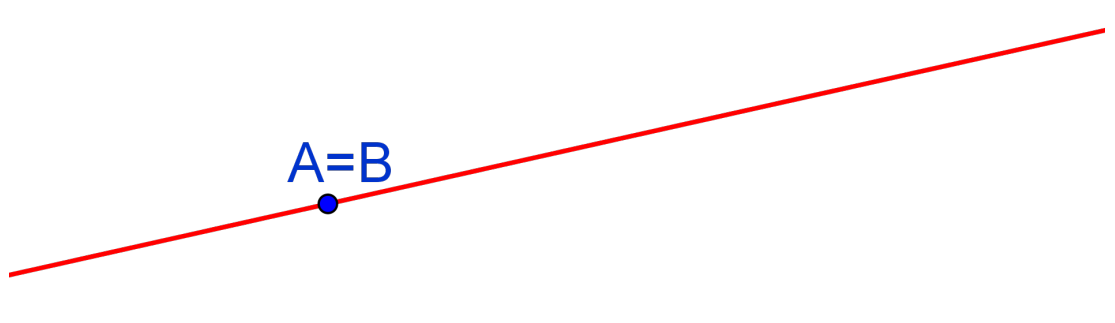
\includegraphics[scale=0.2]{Trabajos/11/Envios/Ax1a.PNG}
		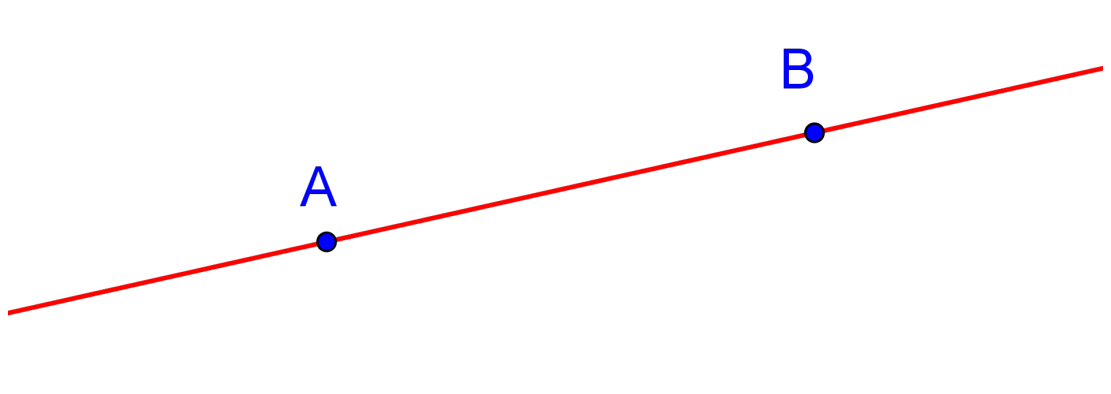
\includegraphics[scale=0.2]{Trabajos/11/Envios/Ax1b2b.PNG}
	\end{figure}
	
	\item Registro simbólico: Podemos usar símbolos matemáticos para expresar el axioma, por ejemplo: $\forall A \forall B \exists r \bigl( P(A,B) \rightarrow \mathcal{R}(r) \wedge A,B \in r \bigr)$
	
	\item Registro manipulativo: Podemos utilizar regla y compás para construir físicamente una línea que pase por los puntos $A$ y $B$.
	
	\item Registros computacionales: Con el uso de Geogebra, se puede realizar dibujos dinámicos, es decir que en este caso pudiera cambiarse las posiciones relativas de $A$ y de $B$ y ver el cambio de la línea que pasa por $A$ y por $B$. Para más ejemplos de este recurso puede verse \cite{geometria11congeogebra11}.
\end{itemize}

Es común interpretar de la representación lingüística de este axioma que los puntos $A$ y $B$ son distintos. En esta formulación de los axiomas de incidencia, no se especifica explícitamente que los puntos $A$ y $B$ deben ser distintos y, por lo tanto, permite la posibilidad de que $A$ y $B$ sean el mismo punto. Sin embargo, en el caso de la representación simbólica, y con un pequeño auxilio de la lógica, se despejan las dudas. Por ejemplo, revisando la siguiente demostración con el uso del registro simbólico queda claro una implicación de este axioma:
\begin{teorema}
	Si existe un punto, existe una recta: $\vdash\exists A \mathcal{P}(A) \rightarrow \exists r \mathcal{R}(r)$
\end{teorema}

\begin{proof}
	~
	
	\begin{center}
		\def\arraystretch{1.5}
		\begin{tabular}{|c|l|c|}
			\hline 
			1. & $\exists A \mathcal{P}(A)$ & as\\
			\hline 
			2. & $\mathcal{P}(A)$ & c$A$\\
			\hline 
			3. & $\forall A \forall B \exists r \bigl( \mathcal{P}(A,B) \leftarrow \mathcal{R}(r) \wedge A,B \in r \bigr)$ & ax1\\
			\hline 
			4. & $\exists \bigl( \mathcal{P}(A,A) \leftarrow \mathcal{R}(r) \wedge A,A \in r \bigr)$ & spec\\
			\hline 
			5. & $\mathcal{P}(A,A) \rightarrow \mathcal{R}(r) \wedge A,A, \in r$ & c$r$\\
			\hline 
			6. & $\mathcal{R}(r)$ & SC 2,5\\
			\hline 
			7. & $\exists r \mathcal{R}(r)$ & $\exists$\\
			\hline 
			8. & $\exists r \mathcal{R}(r)$ & c5\\
			\hline 
			9. & $\exists r \mathcal{R}(r)$ & c2\\
			\hline 
			10. & $\exists A \mathcal{P}(A) \rightarrow \exists r \mathcal{R}(r)$ & DT 1-9\\
			\hline 
		\end{tabular}
	\end{center}
	
\end{proof}

En esta demostración solamente usamos el axioma propio 1, además de metateoremas del cálculo de predicados con la igualdad. Una explicación puede ser la siguiente:
\begin{enumerate}
	\item Se supone la existencia de un punto $A$ ($\exists A$) y se afirma que es un punto ($\mathcal{P}(A)$).
	\item Se introduce la notación “cA” para denotar el uso de la regla $C$.
	\item Se utiliza el primer axioma de incidencia.
	\item Se realiza una instancia de cuantificador universal, reemplazando $B$ por $A$ en el axioma, es decir especializando el axioma.
	\item Se utiliza nuevamente la regla C pero esta vez en $r$.
	\item Se utiliza un silogismo o un teorema del calculo de proposiciones (SC) para concluir que $r$ es una recta.
	\item Se utiliza la introducción del cuantificador existencial para afirmar que existe una recta $r$. 
	\item Se descarga la regla C aplicada a $r$.
	\item Se descarga la regla C aplicada a $A$.
	\item Se aplica el teorema de la deducción y se concluye.
\end{enumerate}

\subsection{Bibliografía}

% \nocite{*}
\printbibliography[keyword={11}]
	\clearpage
	%-------------------------------------------------------------------------
% INFORMACIÓN DEL ARTÍCULO
\thispagestyle{portadapage}
\setcounter{subsection}{0}
\setcounter{subsubsection}{0}
\setcounter{actividad}{0}
\setcounter{actividad_previa}{0}
\setcounter{actividad_entre}{0}
\renewcommand{\articulotipo}{Comunicación breve}
\renewcommand{\articulotitulo}{Enseñanza de funciones exponenciales y logarítmicas mediada por tecnologías digitales: relato y conclusiones de una experiencia áulica}
\renewcommand{\articulotitulocorto}{Enseñanza de funciones exponenciales y logarítmicas mediada por tecnologías digitales}
\section{\articulotitulo}
\desctotoc{Del Valle Vides, C. N.}

\noindent\rule{\linewidth}{2pt}

\vspace{0.25cm}

\begin{flushright}
	\addautor[cinthia.vides@exa.unsa.edu.ar]{Cinthia Noelia Del Valle Vides}{Universidad Nacional de Salta}
\end{flushright}

\vspace{0.5cm}

\begin{center}
	\begin{minipage}{0.75\linewidth} \small
		\textsc{Resumen}. ~
		En esta comunicación, se describe una experiencia áulica desarrollada durante la Pasantía Profesional de la Especialización en Educación Mediada por Tecnología Digital de la Universidad Nacional del Comahue. La pasantía se llevó a cabo en la Universidad Nacional de Salta en la asignatura ""Introducción a la Matemática"". Dicho proyecto abordó la enseñanza de funciones exponenciales y logarítmicas mediada por tecnologías digitales, incluyendo Moodle, Geogebra, Chat GPT, Photomath y Whatsapp. Además se justificará la propuesta desde diferentes autores de educación mediada por tecnología digital.
		
		Los resultados de la experiencia mostraron una mejor comprensión de los conceptos matemáticos, mayor participación activa y desarrollo de competencias digitales. Este enfoque demostró cómo la mediación tecnológica puede superar barreras en la enseñanza de la matemática y optimizar el proceso educativo.
	\end{minipage}
\end{center}
%-------------------------------------------------------------------------

\subsection{Introducción}

En la presente comunicación expondré la descripción de una experiencia áulica en el marco de la realización de la Pasantía Profesional correspondiente a la carrera Especialización en Educación Mediada por Tecnología Digital de la Universidad Nacional del Comahue (Carrera con modalidad virtual). Esta Pasantía profesional se desarrolló en la Universidad Nacional de Salta- Facultad de Ciencias Exactas dentro de la asignatura Introducción a la matemática.

La realización de dicha pasantía consistió en la ejecución de un Proyecto Integrador de Saberes, que surgió como un intento de resolver el siguiente problema planteado al inicio del mismo:

\paragraph*{Problema:} “La enseñanza tradicional de la matemática en el nivel universitario no contribuye a superar las dificultades que se presentan en el aprendizaje de las funciones exponenciales y logarítmicas y no se pone en práctica la utilización de herramientas digitales como una alternativa que puede contribuir a superar dichas dificultades”

Ante esta problemática se pensó en una propuesta didáctica que incorporó algunos componentes del ABP (Aprendizaje Basado en Proyectos) asistido por TIC de acuerdo con lo planteado por \textcite{marti2010}, con el fin de mejorar la habilidad para resolver problemas y desarrollar tareas complejas, mejorar la capacidad de trabajar en equipo, aumentar el conocimiento y habilidad en el uso de las TIC en un ambiente de proyectos, incrementar las capacidades de análisis y síntesis, etc.

Sin embargo, esta propuesta no constituyó netamente un aprendizaje basado en proyectos (ABP) puesto que no fue del todo constructivista, sino que la base de la enseñanza de los conceptos matemáticos propiamente dichos siguió un modelo de enseñanza basado en clases teóricas y luego prácticas.

Los aportes del ABP se vieron reflejados en las actividades que se propusieron para lograr lo mencionado anteriormente. No obstante, este proyecto integró saberes que permitieron que los estudiantes pongan en relación los elementos teóricos y prácticos de más de una disciplina, en este caso la matemática y competencias digitales en relación al uso de Tics, teniendo en cuenta lo que plantean \textcite{torres2019}.

Además, como lo exponen \textcite{galvis2013}, las plataformas educativas pueden ser utilizadas como soporte para el desarrollo de Entornos Virtuales de Enseñanza-Aprendizaje permitiendo la inclusión de materiales multimediales diversos, el acceso a múltiples fuentes de información y la comunicación e interacción sincrónicas y asincrónicas. Estas plataformas permiten asimismo potenciar intencionalidades pedagógicas que recuperen el rol protagónico y activo de los estudiantes en los procesos de aprendizaje. Como base del EVEA de este proyecto se propuso el uso de la plataforma Moodle y un canal de comunicación con los estudiantes por medio de un grupo de Whatsapp.

\textcite{area2012} por su parte mencionan que la alfabetización digital debe representar un proceso de desarrollo de una identidad como sujeto en el territorio digital, que se caracterice por la apropiación significativa de las competencias intelectuales, sociales y éticas necesarias para interactuar con la información y para recrearla de un modo crítico y emancipador. Teniendo en cuenta estas ideas se pensó en una propuesta en la que el alumno utilice algunas herramientas como el software Geogebra para graficar funciones, Chat GPT para resolver problemas y elaborar conclusiones, la calculadora digital Photomath para comparar resultados y detectar errores en el procedimiento de resolución de ecuaciones exponenciales y logarítmicas. De esta manera, aquí no solo está de fondo lo referente a dicha alfabetización digital, sino que también se encuentran elementos de la multialfabetización como por ejemplo la alfabetización social. Además, el uso de estas herramientas les permitió desarrollar la capacidad de criticar y evaluar la información que se obtuvo.

En este aspecto, autores de Educación Matemática como por ejemplo \textcite{deguzman2004} ya aseguraba que hay que poner el acento en la comprensión de los procesos matemáticos más bien que en la ejecución de ciertas rutinas que en nuestra situación actual ocupan todavía gran parte de la energía de nuestros alumnos, con el consiguiente sentimiento de esterilidad del tiempo que en ello emplean y que lo verdaderamente importante vendrá a ser su preparación para el diálogo inteligente con las herramientas que ya existen, de las que ya disponen. Si bien el en su tiempo se refería a las calculadoras y los ordenadores que recién estaban apareciendo sus palabras hoy están más que vigentes considerando las herramientas digitales actuales que facilitan el trabajo en las aulas y fuera de ellas y seguramente seguirán estando vigentes para las herramientas que vendrán en el futuro.

Por otro lado \textcite{garcia2020} se enfocan específicamente en el uso del Geogebra para el aprendizaje de las funciones exponenciales mediante el uso de deslizadores que permiten identificar cómo varía la gráfica de una función exponencial de la forma $f(x) = k a^x + b$ al variar los parámetros $a$, $k$, y $b$. Es por ello que se dedicó un tiempo de clase especial a que los alumnos puedan explorar un recurso de Geogebra asociado a un código QR para establecer conclusiones sobre la imagen, asíntotas, intervalos de crecimiento y/o decrecimiento de la función exponencial, intersecciones con los ejes, etc. de acuerdo a la variación de dichos parámetros teniendo en cuenta que sin el uso de este recurso sería muy difícil que los alumnos pudieran establecer estas conclusiones de manera autónoma sin que el docente tuviera que dictarle las respuestas.

\subsection{Contenidos}

El contenido principal de esta comunicación será el aprendizaje de las Funciones Exponenciales y Logarítmicas mediado por tecnologías digitales a partir de una experiencia áulica llevada a cabo en una asignatura de Matemáticas previas al Cálculo. El Proyecto Integrador de Saberes que dió origen a la experiencia áulica integró los contenidos matemáticos de Logaritmo y propiedades, Funciones Exponenciales y Logarítmicas y Aplicaciones de la Función Exponencial con cuestiones teóricas y prácticas respecto a la mediación de tecnologías digitales en la enseñanza.

\subsection{Objetivos}

\begin{itemize}
	\item Fortalecer los espacios de aprendizaje de las funciones exponenciales y logarítmicas a través de la mediación digital.
	\item Compartir una experiencia exitosa de integración de tecnologías digitales en la enseñanza de la matemática.
	\item Mostrar cómo las herramientas digitales pueden superar barreras epistemológicas en la enseñanza de funciones exponenciales y logarítmicas.
	\item Reflexionar sobre cómo la mediación tecnológica puede mejorar la organización de las clases y optimizar tiempos en la enseñanza de la	matemática.
	\item Inspirar a otros educadores a incorporar tecnologías digitales en sus prácticas de enseñanza para mejorar el aprendizaje de los estudiantes.
\end{itemize}

\subsection{Desarrollo de la comunicación}

Para el desarrollo de la comunicación se utilizarán diapositivas, las cuales tendrán palabras y conceptos claves para desarrollar los siguientes punto de dicha comunicación:

\begin{enumerate}[I.]
	\item \textbf{Contexto y Justificación}: Se describirá el contexto en el que se realizó la Pasantía Profesional, es decir la institución, asignatura, características del grupo clase, trabajo previo con tecnologías digitales, etc. Además se justificará desde diferentes autores de matemática, educación matemática y educación mediada por tecnología digital la elaboración de la propuesta didáctica del proyecto y particularmente la mediación tecnológica en la enseñanza de los contenidos matemáticos mencionados.
	\item \textbf{Actividades y Herramientas Digitales Utilizadas}: Se realizará una descripción de las actividades desarrolladas y de las herramientas digitales y recursos digitales utilizados. Entre dichas herramientas se destacan las siguientes:
	\begin{itemize}
		\item \textit{Plataforma Moodle}: Utilizada para compartir materiales didácticos y crear actividades evaluativas. Dentro de los recursos propios de moodle se utilizaron “Libro”, “Cuestionario” “Tarea”, “Carpeta”, etc. En particular se destaca el recurso Libro que recopiló las principales producciones de los estudiantes, algunas orientaciones para el desarrollo de actividades propuestas y recursos elaborados para favorecer la comprensión de los alumnos. De esta manera, aquellos estudiantes que por diversos factores no pudieron asistir a clases tuvieron al alcance una herramienta que les permitiera plantear y resolver los principales ejercicios del TP en conjunto con las diapositivas de clases prácticas.
		\item \textit{Presentación con diapositivas}: Se utilizaron diapositivas que contenían los principales conceptos teóricos y los ejercicios prácticos a desarrollar en el pizarrón (que fueron completados en las mismas diapositivas con una pizarra electrónica).
		\item \textit{Geogebra}: Proporcionó recursos interactivos para la visualización y manipulación de funciones exponenciales, permitiéndoles a los estudiantes observar como varían los parámetros de una función exponencial de la forma $f(x) = k a^x + b$. Además se aprovecharon sus facilidades para la verificación de resultados en el análisis de funciones exponenciales y logarítmicas y para visualizar cómo determinadas funciones exponenciales pueden modelar ciertas situaciones problemáticas.
		\item \textit{Chat GPT}: Herramienta utilizada para resolver problemas del tipo “Obtener una función de tipo exponencial que cumpla las siguientes condiciones”, analizando de manera crítica si las respuestas que esta IA les proporcionaba eran correctas con sus correspondientes justificaciones.
		\item \textit{Photomath}: Aplicación utilizada para la verificación de resultados y procedimientos en la resolución de ecuaciones exponenciales y logarítmicas.
		\item \textit{Whatsapp}: Las interacciones en el grupo de Whatsapp permitieron mantener una comunicación constante fluida y dinámica con los estudiantes, creando también un espacio de trabajo colaborativo en el que se compartieron ejercicios, dudas, correcciones, etc.
		\item \textit{Video Educativo}: Creación de videos específicos que abordaban conceptos clave de las funciones exponenciales y logarítmicas, permitiendo a los estudiantes revisar los temas a su propio ritmo.
		\item \textit{Zoom}: Para una clase virtual extra en la que se resolvieron ejercicios integradores de exámenes parciales de años anteriores.
	\end{itemize}
	\item \textbf{Resultados y conclusiones}: En este momento se expondrán las principales conclusiones y logros obtenidos a partir de la ejecución del Proyecto Integrador de Saberes propuesto. Entre ellos, se destaca que la integración de tecnologías digitales permitió:
	\begin{itemize}
		\item \textit{Mejor comprensión}: Los estudiantes mostraron una mejor comprensión de las funciones exponenciales y logarítmicas, como se evidenció en las actividades evaluativas, en los ejercicios compartidos y en los desarrollos que se observaron en clase.
		\item \textit{Participación Activa}: Aumento en la participación de los estudiantes en discusiones y actividades en línea.
		\item \textit{Desarrollo de Competencias Digitales}: Los estudiantes adquirieron habilidades digitales útiles para resolver problemas matemáticos y para su desempeño académico y profesional en general.
	\end{itemize}
\end{enumerate}

\subsection{Bibliografía}

\nocite{*}
\printbibliography[keyword={12}]
	\clearpage
	%-------------------------------------------------------------------------
% INFORMACIÓN DEL ARTÍCULO
\thispagestyle{portadapage}
\setcounter{subsection}{0}
\setcounter{subsubsection}{0}
\setcounter{actividad}{0}
\setcounter{actividad_previa}{0}
\setcounter{actividad_entre}{0}
\renewcommand{\articulotipo}{Comunicación breve}
\renewcommand{\articulotitulo}{La cota de Lamé}
\renewcommand{\articulotitulocorto}{La cota de Lamé}
\section{\articulotitulo}
\desctotoc{Zivec, R.}

\noindent\rule{\linewidth}{2pt}

\vspace{0.25cm}

\begin{flushright}
	\addautor[ricardo.zivec@unsta.edu.ar]{Ricardo Zivec}{Facultad de Ingeniería - Universidad del Norte Santo Tomas de Aquino}
\end{flushright}

\vspace{0.5cm}

\begin{center}
	\begin{minipage}{0.75\linewidth} \small
		\textsc{Resumen}. ~
		El teorema de la cota de Lamé, es un resultado en teoría de números que proporciona una cota superior para el número de pasos necesarios en el algoritmo de Euclides para encontrar el (MCD) de dos números naturales.
	\end{minipage}\\
	
	\vspace{0.5em}
	
	\begin{minipage}{0.75\linewidth} \small
	\textsc{Palabras clave} --- Comprensión, Análisis, Preparación pedagógica
	\end{minipage}
\end{center}
%-------------------------------------------------------------------------

\subsection{Introducción}

El teorema de la cota de Lamé, es un resultado en teoría de números que proporciona una cota superior para el número de pasos necesarios en el algoritmo de Euclides para encontrar el (MCD) de dos números naturales.

En la comunicación se dará una descripción general, de la importancia de la enseñanza a futuros docentes en matemáticas, la cuál es crucial por 4 razones: Profundización en la teoría de números, eficiencia algorítmica, preparación para la enseñanza, pensamiento crítico y analítico.

\subsection{Objetivos}

Este trabajo tiene como objetivos;
\begin{enumerate}
	\item 1. Comprensión Teórica: Lograr que los estudiantes comprendan el enunciado y la demostración del teorema de Lame.
	\item Aplicación Práctica: Desarrollar habilidades para aplicar el algoritmo de Euclides en la determinación del MCD y entender su eficiencia.
	\item Análisis Crítico: Fomentar la capacidad de analizar la complejidad y la importancia de la eficiencia en matemáticas.
	\item Preparación didáctica: Preparar a los estudiantes para enseñar estos conceptos a nivel escolar, explicándoles de manera clara y accesible.
\end{enumerate}

\subsection{Contenidos}
\begin{itemize}
	\item Introducción al algoritmo de Euclides.
	\item Enunciado del Teorema de Lamé: Demostración y ejemplos prácticos
	\item Análisis de eficiencia.
	\item Métodos de enseñanza.
\end{itemize}

En definitiva, la enseñanza del Teorema de Lamé a futuros profesores de matemáticas no solo enriquece su conocimiento teórico y práctico, sino que también mejora su capacidad para transmitir estos conceptos, fomentando una educación matemática más sólida y profunda.

\subsection{Bibliografía}

\nocite{*}
\printbibliography[keyword={13}]
	\clearpage
	%-------------------------------------------------------------------------
% INFORMACIÓN DEL ARTÍCULO
\thispagestyle{portadapage}
\setcounter{subsection}{0}
\setcounter{subsubsection}{0}
\setcounter{actividad}{0}
\setcounter{actividad_previa}{0}
\setcounter{actividad_entre}{0}
\renewcommand{\articulotipo}{Comunicación breve}
\renewcommand{\articulotitulo}{Matemática, uno de los ejes principales en la Feria de Ciencias STEAM}
\renewcommand{\articulotitulocorto}{Matemática, uno de los ejes principales en la Feria de Ciencias STEAM}
\section{\articulotitulo}
\desctotoc{Céliz, Z. F.; Shneider, E.}

\noindent\rule{\linewidth}{2pt}

\vspace{0.25cm}

\begin{flushright}
	\addautor[zulmaceliz@gmail.com]{Zulma Fabiana Céliz}{-}
	\vspace{1em}
	\addautor[]{Ernesto Shneider}{-}
\end{flushright}

\vspace{0.5cm}

\begin{center}
	\begin{minipage}{0.75\linewidth} \small
		\textsc{Resumen}. ~
		Las Ferias de Ciencias, estrategia pedagógica implementadas en comunidades educativas en los distintos niveles y modalidades, públicas y privadas, se instalan en ellas para la mejora de los aprendizajes y de optimización de la enseñanza.
		
		En este año se espera que los proyectos feriales se fundamenten y desarrollen desde la perspectiva STEAM situada, adaptada al Nivel y Modalidad Educativa y al contexto de la escuela/comunidad donde se genera y desarrolla.
		
		La metodología STEAM, modelo educativo que promueve la integración de las áreas científicas, tecnológicas, matemática y artísticas en un único marco interdisciplinar, busca el desarrollo de habilidades en los alumnos de las distintas áreas, fomentar el pensamiento crítico y el razonamiento lógico. Se destacará la importancia de la Matemática como uno de los ejes principales de ésta metodología y que servirá para vertebrar los proyectos integrados y la construcción del aprendizaje autónomo y crítico.
	\end{minipage}
\end{center}
%-------------------------------------------------------------------------

\subsection{Introducción}

El enfoque STEAM se presenta como un conjunto de didácticas (singulares, innovadoras) que prioriza la actividad de los estudiantes de modo interdisciplinario y contextualizado por medio de la resolución de problemas, basados en el planteo y desarrollo de múltiples y variados proyectos de aula. Basado en los cambios de patrones o estándares que surgen de las necesidades emergentes de la sociedad y de la baja tendencia de sus indicadores económicos, ya que busca no solo ofrecer conocimientos específicos de cada disciplina, sino también promover habilidades y capacidades en un permanente ecosistema de aprendizaje.

Propone entre otros: mejorar la calidad de las experiencias de aprendizaje de los alumnos (Rogers, 2005); aumentar el interés de los estudiantes, mejorar los saberes en las prácticas de alfabetización y demostrar la utilidad de las matemáticas y las ciencias (Gattie y Wicklein, 2007); mejorar la alfabetización tecnológica (Rogers, 2005).

La feria de ciencias brinda la oportunidad para la construcción, implementación y evaluación del enfoque STEAM. En la actualidad las ferias de ciencias incluyen proyectos de todas las áreas curriculares y se extienden a todos los niveles y modalidades del sistema educativo nacional.

Cada feria propicia que el foco de todos los proyectos y actividades que en ella se presenten se encuentren en los contenidos de los diseños curriculares correspondientes a cada una de las jurisdicciones, en los Núcleos de Aprendizajes Prioritarios (NAP) y aquellos documentos que regulen la enseñanza en cada contexto educativo.

Las ferias forman parte de la planificación escolar y pueden considerarse un enfoque educativo con objetivos didácticos asociados al cotidiano de la escuela, a la enseñanza y, fundamentalmente, a la integración de aprendizajes. Resultan un enfoque que apunta a su mejora, es decir, al aumento y la promoción en la calidad de habilidades y capacidades de quienes forman parte del proyecto educativo. Reflejan la integración en la construcción y reconstrucción del conocimiento escolar. Asimismo, el proyecto se retroalimenta dando relevancia a la evaluación formativa, optimizan el proceso en constante enriquecimiento del proyecto final.

Los eventos de feria de ciencias se orientan por las normas escolares, la convivencia escolar, los diseños curriculares jurisdiccionales y los documentos federales y nacionales. Se integran ferias de ciencias semejantes de otros países. Se constituyen como un evento lejano a una competencia de equipos o una contienda de logros individuales. En las ferias no se rinde examen, no hay pruebas a superar, sino saberes por construir y reconstruir en un proceso educativo integrado. Al exhibir la producción se genera un reconocimiento auténtico del proyecto de ferias, ya que se comparte con otros actores de la escuela, de la localidad, de la jurisdicción y, al final de su recorrido, del país y posiblemente también del extranjero.

Para el Programa Nacional de Ferias de Ciencias y Tecnología la base epistémica de una propuesta STEAM es el “aprender a aprender”, ya que reconoce que el proceso de aprender no se limita simplemente a adquirir conocimientos y habilidades específicas en áreas particulares, sino que implica también desarrollar habilidades metacognitivas, capacidades de resolución de problemas y disposiciones para el aprendizaje continuo y adaptativo. Para esto recurrimos a dos planteos teóricos: el aprendizaje significativo y el aprendizaje crítico.

Parafraseando la obra de Paulo Freire concluimos que en una feria de ciencias es evidente que quienes enseñan, aprenden al enseñar; y quienes aprenden, enseñan al aprender. El conocimiento no es transmitido, sino que se construye o se produce, y tanto el educando como el educador deben percibirse y asumirse como sujetos activos en el proceso de construcción. Por lo que las ferias de ciencias proponen un escenario propicio para la proyección de una estrategia “STEAM situada”, dado que las características de sus trabajos y su evaluación proporcionan experiencias concretas atentos a los retos que nuestro sistema educativo debe afrontar.

Unos de los ejes principales de la metodología STEAM, MATEMATICA, que podrá tenerse en cuenta como vertebrador de éstos proyectos para los trabajos de Feria integrándose con otros campos curriculares de los otros ejes, para los cuales se considera: cómo se construye y reconstruye el conocimiento escolar, cómo se elaboran y reelaboran los saberes desde el aula, la valoración realizada, apropiación y desarrollo creativo del trabajo, con relación a ámbitos naturales o culturales, la realización o promoción de aportes a los procesos de enseñanza y aprendizaje, a la vida institucional de los establecimientos educativos de pertenencia de la zona y la vinculación del proyecto con el contexto social. Los trabajos que tengan como punto de partida el eje MATEMATICO deben ser formulados sobre temas curriculares vinculados con Aritmética, Álgebra, Cálculo, Geometría, Estadística, Probabilidades, pero también sobre temas que articulan con Topología, y aplicaciones matemáticas en otras áreas que a partir del abordaje de una problemática compleja articulen aspectos matemáticos para su planteo o resolución. También Historia de la Matemática podrá se considerarse vinculada con el área de matemática. Se diferenciarán tres tipos de proyectos matemáticos: los relacionados con el uso de la Matemática en otras áreas de conocimiento, aquellos relacionados con problemas matemáticos y los vinculados con la historia de la matemática. Los cuales deberán cumplir con ciertos criterios específicos: significatividad del problema elegido y pertinencia del análisis realizado, delimitación del problema de otra área a cuya comprensión aporta la matemática mediante el uso de modelos matemáticos, relevancia del problema elegido, utilización pertinente de diferentes modelos matemáticos al resolver el problema y uso adecuado de representaciones; claridad en la comunicación de los procedimientos utilizados y las nociones matemáticas involucradas; explicitación de manera clara y completa de las formas de resolución y de las nociones y propiedades involucradas, utilizando el lenguaje en forma adecuada; presentación, detalle, dibujos y gráficos; ordenamiento y sistematización; utilización pertinente de diferentes modelos matemáticos al resolver el problema; indagación sobre una noción en distintos momentos históricos, en el marco de las ideas de su tiempo.\footnote{Tomado de los documentos 1, 2, y 3 del Material del Programa Nacional de Feria de Ciencias}.

\subsection{Contenidos}

Feria de Educación, Ciencia, Arte, y Tecnología de la Provincia. Feria de Ciencia STEAM Situada. Eje Matemático y foco principal en el desarrollo de Proyecto de Feria de Ciencias.

\subsection{Objetivos}
\begin{itemize}
	\item Destacar la importancia de la Matemática como eje vertebrador de un proyecto de Feria de Ciencias STEAM situada, en un proceso en el cual se busca la mejora de la enseñanza y la calidad de los aprendizajes adquiridos.
	\item Visibilizar el trabajo de Feria de Ciencias desarrollada por docentes y alumnos, adoptando y apropiándose de formas efectivas y eficaces de estrategias del proceso de enseñanza/aprendizaje; y que proponen formas superadoras a implementar en la enseñanza de la Matemática.
\end{itemize}

\subsection{Desarrollo de la comunicación}

\begin{itemize}
	\item A cargo de la Profesora Zulma Céliz, exposición sobre Feria de Ciencia, exposición sobre características principales e historia.
	\item Presentación del Profesor Referente Nacional de Evaluación Feria de Ciencia: Ernesto Scheiner
	\item Exposición sobre: “El eje de Matemática en una Feria de Ciencias STEAM situada”.
	\item Recursos: Conexión virtual vía internet. Material de apoyo: diapositivas
\end{itemize}

\subsection{Bibliografía}

\nocite{*}
\printbibliography[keyword={14}]
	\clearpage
	%-------------------------------------------------------------------------
% INFORMACIÓN DEL ARTÍCULO
\thispagestyle{portadapage}
\setcounter{subsection}{0}
\setcounter{subsubsection}{0}
\setcounter{actividad}{0}
\setcounter{actividad_previa}{0}
\setcounter{actividad_entre}{0}
\renewcommand{\articulotipo}{Comunicación breve}
\renewcommand{\articulotitulo}{Retos en la aplicación del aprendizaje basado en problemas en la asignatura Bioestadística y Diseño Experimental}
\renewcommand{\articulotitulocorto}{Retos en la aplicación del aprendizaje basado en problemas en la asignatura Bioestadística y Diseño Experimental}
\section{\articulotitulo}
\desctotoc{Humacata, I. C.; Guzmán, V. R.}

\noindent\rule{\linewidth}{2pt}

\vspace{0.25cm}

\begin{flushright}
	\addautor[ivonehumacata@fca.unju.edu.ar]{Ivone Carolina Humacata}{Facultad de Ciencias Agrarias, Universidad Nacional de Jujuy}
	\vspace{1em}
	\addautor[]{Vilma Roxana Guzmán}{Facultad de Ciencias Agrarias, Universidad Nacional de Jujuy}
\end{flushright}

\vspace{0.5cm}

\begin{center}
	\begin{minipage}{0.75\linewidth} \small
		\textsc{Resumen}. ~
		El Aprendizaje Basado en Problemas (ABP) es una estrategia didáctica innovadora en la enseñanza de Bioestadística y Diseño experimental. Sin embargo, su implementación enfrenta algunos desafíos como la dedicación de más tiempo por parte de estudiantes y docentes, resistencia inicial a la propuesta, necesidad de mayor coordinación grupal y dificultades en el aprendizaje de software estadístico. Para mejorar la aplicación del ABP, se proponen las siguientes estrategias: optimizar la gestión del tiempo, ofrecer cursos complementarios, crear comunidades de aprendizaje docente, conformar grupos reducidos y ofrecer cursos de formación docente y considerar al ABP como una metodología complementaria al método tradicional.
	\end{minipage}\\
	
	\vspace{0.5em}
	
	\begin{minipage}{0.75\linewidth} \small
	\textsc{Palabras clave} --- ABP, estadística, agronomía, estrategias didácticas, educación superior
	\end{minipage}
\end{center}

\vspace{1em}

\begin{center}
	\begin{minipage}{0.75\linewidth} \small
		\textsc{Abstract}. ~
		Problem-Based Learning (PBL) is an innovative teaching strategy in the teaching of Biostatistics and Experimental Design. However, its implementation faces some challenges such as the dedication of more time by students and teachers, initial resistance to the proposal, the need for greater group coordination and difficulties in learning statistical software. To improve the application of PBL, the following strategies are proposed: optimise time management, offer complementary courses, create teacher learning communities, form small groups and offer teacher training courses, and consider PBL as a complementary methodology to the traditional method.
	\end{minipage}\\
	
	\vspace{0.5em}
	
	\begin{minipage}{0.75\linewidth} \small
	\textsc{Keywords} --- BL, statistics, agronomy, teaching strategies, higher education
	\end{minipage}
\end{center}
%-------------------------------------------------------------------------

\subsection{Introducción}

La enseñanza de la estadística en el nivel superior enfrenta desafíos debido a la naturaleza abstracta y conceptual de los conceptos estadísticos. Una de las dificultades identificadas es la tendencia de los estudiantes a memorizar fórmulas y procedimientos sin comprender su significado y aplicabilidad. Esto puede conducir a un aprendizaje superficial y limitado, donde los estudiantes pueden tener dificultades para transferir los conocimientos estadísticos a situaciones reales \textcite{batanero2001}.

En este contexto, el Aprendizaje Basado en Problemas (ABP) surge como una estrategia didáctica, que permite a los estudiantes aplicar sus conocimientos previos, desarrollar competencias específicas y contextualizar su aprendizaje (Kilpatrick, 1918; \textcite{fernandez2013}). En línea con \textcite{vargas2020} “el ABP es una experiencia de aprendizaje que involucra al estudiante en un proyecto complejo y significativo, el cual permite el desarrollo integral de sus capacidades, habilidades, actitudes y valores.” (\textcite[p.~170]{vargas2020}).

La integración del ABP en la enseñanza de Bioestadística y Diseño experimental, en la educación superior, se presenta como una oportunidad para repensar las prácticas docentes y los objetivos de aprendizaje (Vargas et al., 2020). Sin embargo, es necesario identificar los retos y dificultades que enfrentan los docentes y estudiantes al implementar esta estrategia, con el fin de mejorar su aplicación y contribuir al desarrollo de competencias estadísticas y de resolución de problemas en los estudiantes.

El objetivo del presente trabajo fue identificar los retos que enfrenta la aplicación del ABP en la asignatura de Bioestadística y Diseño Experimental, en el nivel de educación superior.

\subsection{Contenidos}

El presente trabajo es de tipo cualitativo transversal. Para la identificación de los desafíos y retos en la implementación del ABP se recurrió a las entrevistas a docentes y estudiantes. Se registraron las entrevistas por medio de grabaciones, posteriormente se transcribieron para su análisis.

Los desafíos identificados en la implementación del ABP en la enseñanza de Bioestadística y Diseño experimental, coinciden con los encontrados en la literatura revisada (\textcite{gonzalezhernando2016, paredescurin2016}):
\begin{itemize}
	\item Requiere más tiempo por parte de los estudiantes, ya que asumen un rol activo y participativo en el proceso de enseñanza-aprendizaje.
	\item Demanda más tiempo del docente en cuanto a tutorías para los grupos, ya que debe diseñar los problemas, preparar material, organizar los grupos y programar el trabajo, supervisarlos y evaluarlos.
	\item Al principio, los estudiantes pueden mostrar rechazo o resistencia a la forma de aprender, al estar acostumbrados a métodos tradicionales.
	\item Es necesaria una mayor coordinación de grupo, en cuanto a las tareas y en el horario para reunirse.
	\item El aprendizaje que propone el ABP puede resultar complejo para los estudiantes, al requerir nuevas habilidades.
	\item Algunos temas conceptuales de la asignatura cobran más relevancia que otros, dependiendo del problema planteado a resolver.
	\item Surgen problemas interpersonales en el grupo, debido a la falta de compromiso o participación en la realización de las actividades asignadas.
	\item Dificultades en el aprendizaje y aplicación del software estadístico R, especialmente en el uso de paquetes, librerías y funciones
\end{itemize}

\subsubsection{Estrategias para mejorar la implementación del ABP}

A partir de los desafíos identificados en la implementación del ABP se proponen las siguientes estrategias para mejorar su aplicación:
\begin{enumerate}
	\item Optimizar la gestión del tiempo de clases, mediante la creación de videos tutoriales que permitan a los estudiantes acceder a material de apoyo de manera asincrónica.
	\item Ofrecer cursos curriculares complementarios para el uso de software estadístico.
	\item Crear comunidades de aprendizaje docente que fomenten espacios de reflexión y discusión sobre las prácticas de enseñanza-aprendizaje basadas en el ABP.
	\item Conformar grupos de trabajo reducidos (hasta 3 integrantes) y permitir que los estudiantes elijan libremente a sus compañeros.
	\item Ofrecer cursos de formación docente para los docentes, con el fin de profundizar en la implementación de estrategias didácticas como el ABP en Bioestadística y diseño experimental.
	\item Considerar el ABP como una metodología docente complementaria al método tradicional.
\end{enumerate}

\subsection{Objetivos}

\subsubsection{General}

Identificar los retos que enfrenta la aplicación del Aprendizaje Basado en Problemas (ABP) en la asignatura de Bioestadística y Diseño Experimental en el nivel de educación superior.

\subsubsection{Específicos}

\begin{itemize}
	\item Identificar las principales dificultades y desafíos que enfrentan los docentes y los estudiantes al implementar el ABP en la enseñanza de Bioestadística y Diseño Experimental.
	\item Proponer estrategias para mejorar la aplicación del ABP en la enseñanza de Bioestadística y Diseño Experimental.
\end{itemize}

\subsection{Desarrollo de la comunicación}

\subsubsection{Introducción (2 minutos)}

\begin{itemize}
	\item Presentación del tema y objetivos de la comunicación breve.
	\item Contextualización de la importancia del tema en el campo de estudio.
\end{itemize}

\subsubsection{Desarrollo (10 minutos)}

\begin{itemize}
	\item Definición y características del Aprendizaje Basado en Problemas (ABP).
	\item Explicación del ABP como estrategia didáctica.
	\item Ventajas y beneficios del ABP en la enseñanza de Bioestadística y Diseño Experimental.
	\item Identificación de los principales desafíos para los docentes y los estudiantes.
	\item Sugerencias y recomendaciones para superar las dificultades identificadas.
\end{itemize}

\subsubsection{Conclusión (1 minuto)}

\begin{itemize}
	\item Resumen de los principales puntos abordados.
	\item Reafirmación de la importancia del tema y sus implicaciones en la enseñanza de Bioestadística y Diseño Experimental.
\end{itemize}

\subsubsection{Material de apoyo}

\begin{itemize}
	\item Uso de diapositivas para resaltar los puntos clave.
\end{itemize}

\subsection{Bibliografía}

\nocite{*}
\printbibliography[keyword={15}]
	\clearpage
	%-------------------------------------------------------------------------
% INFORMACIÓN DEL ARTÍCULO
\thispagestyle{portadapage}
\setcounter{subsection}{0}
\setcounter{subsubsection}{0}
\setcounter{actividad}{0}
\setcounter{actividad_previa}{0}
\setcounter{actividad_entre}{0}
\renewcommand{\articulotipo}{Comunicación breve}
\renewcommand{\articulotitulo}{Matemática y brotes epidémicos en localidades de Salta: Acciones desde el ámbito educativo}
\renewcommand{\articulotitulocorto}{Matemática y brotes epidémicos en localidades de Salta: Acciones desde el ámbito educativo}
\section{\articulotitulo}
\desctotoc{Humacata, I. C.; Guzmán, V. R.}

\noindent\rule{\linewidth}{2pt}

\vspace{0.25cm}

\begin{flushright}
	\addautor[pablofernando300494@gmail.com]{Pablo Fernando	Quintana}{-}
	\vspace{1em}
	\addautor[]{Emanuel Osedo}{-}
\end{flushright}

\vspace{0.5cm}

\begin{center}
	\begin{minipage}{0.75\linewidth} \small
		\textsc{Resumen}. ~
		La modelización de epidemias se ha convertido en un tema de actualidad con la pandemia de 2020 causada por un coronavirus. Nociones técnicas como el parámetro $R_0$, número reproductivo básico, han aparecido en el discurso de los responsables políticos más importantes de todos los países afectados en el mundo.
		
		El concepto de $R_0$ elemental conlleva la idea básica de una progresión geométrica, a una exponencial, del número de casos. Se trata de una especie de promedio, que, por lo general, no resulta un número entero.
		
		En este trabajo se presentan aplicaciones de la matemática en epidemias, se analizan algunos brotes epidémicos y estimaciones de parámetros de enfermedades transmitidas por vectores en localidades de Salta. Se discuten algunas experiencias para la incorporación de la temática en el ámbito educativo. Se comentan resultados del impacto de acciones en la formación de recursos humanos y su divulgación en distintos niveles educativos.
	\end{minipage}
\end{center}
%-------------------------------------------------------------------------

\subsection{Introducción}

El 11 de marzo de 2020, el Director General de la Organización Mundial de la Salud (OMS), Dr. Ghebreyesus, anunció que la nueva enfermedad por el coronavirus 2019 (COVID-19) puede caracterizarse como una pandemia. La caracterización de pandemia significa que la epidemia se ha extendido por varios países, continentes o todo el mundo, y que afecta a un gran número de personas. Los habitantes del mundo en ese lapso pudieron experimentar el peligro de lo que significa una pandemia, cuando se trata de enfermedades para las cuales no existen tratamientos, remedios o vacunas para enfrentar este tipo de amenaza a toda la humanidad.

En 1920 el demógrafo Alfred Lotka propuso la idea seminal del número de reproducción, como una medida de la tasa de reproducción de una población determinada. En los años 50, del siglo XX, el epidemiólogo George MacDonald sugirió usarlo para describir el potencial de transmisión de la malaria. Propuso que si $R_0$ es menor que 1, entonces la enfermedad va a desaparecer en una población. Las autoridades sanitarias realizan esfuerzos ante un brote epidémico, para intentar reducir el valor de $R_0$ para que sea inferior a 1.

Sin embargo las estimaciones se basan en escenarios teóricos dependientes de los diferentes modelos que pudieran surgir para el análisis de propagación de una enfermedad.

En éste sentido la formación de recursos humanos y la capacitación que ameritan modelos más complejos precisan de un fortalecimiento de acciones por parte de las instituciones educativas. Surge nuevamente la importancia de la interdisciplinariedad que juega la Matemática como soporte de las diferentes ciencias que hacen uso de las diversas herramientas que proporcionan los métodos de la Matemática Aplicada.

\subsection{Contenidos}

En ésta sección presentamos los contenidos que constituyen esta comunicación.

\subsubsection{Brotes epidémicos del Covid en Campo Quijano, Dengue en Cafayate}

El COVID 19 es una enfermedad respiratoria causada por el virus SARS-COV2. Este virus pertenece a la familia de los coronavirus que causan habitualmente enfermedades inofensivas para las personas como los resfriados, aunque existen los que pueden causar infecciones más graves como el llamado SARS (síndrome agudo respiratorio). Este virus causa una forma grave de neumonía, el cual provoca brotes epidémicos desde el año 2003 (\url{https://www.paho.org/es/temas/coronavirus}). En el caso de campo Quijano hubo un registro de datos de los primeros 40 días, posteriormente el sistema de testeo quedó colapsado ya que los casos eran cada vez mayores y los tests no eran de realización exclusiva del hospital sino que podrían hacerse en laboratorios privados y los resultados no eran informados.

En lo que respecta al Dengue, durante el periodo de vigilancia 2023-2024, según el Ministro de Salud Pública de Salta, en la provincia se notificaron 25.237 positivos. El aumento fue de 9.467 casos respecto al periodo anterior, en el que hubo 15.770, lo que significa un incremento del 60\% de los casos. En particular, en Cafayate, se registraron 399 casos. Llama la atención la extensión hacia departamentos de Salta que antes tenían baja incidencia y solía concentrarse en el norte provincial, en los departamentos San Martín, Orán y Anta.

\subsubsection{Matemática aplicada, modelización matemática de epidemias. Modelos clásicos. El modelo exponencial. El modelo SIR. El número de reproducción básico}

El modelo exponencial es conocido, prácticamente por alumnos de los niveles secundario, terciario y universitario. Por lo general, el sentido en las actividades de enseñanza-aprendizaje siempre es desde las expresiones funcionales a sus gráficas. El cambio de paradigma que se propone, siempre que sea posible es, ir de los datos a la obtención de las expresiones funcionales.

El modelo SIR se considera el más simple de los modelos para describir una epidemia, tiene en cuenta una población homogénea y está compuesto por tres ecuaciones diferenciales ordinarias en compartimientos que describen la dinámica de los contagios. Sus siglas se refieren a $S$ (susceptibles), $I$ (infectados) y $R$ (recuperados o removidos). En él se consideran parámetros como la tasa de transmisión y tasa de recuperación las cuales permiten calcular el número de reproducción básico $R_0$.

A partir de estos modelos es posible llevar a cabo el análisis de listas de datos en función del tiempo, por lo general días o semanas epidemiológicas, para lograr probables curvas o distribución del número de casos o incidencias o alguna transformación con el objeto de suavizar las descripciones encontrar que facilitan su análisis.

Con los datos es posible, recurrir a elementos de estadística descriptivas, estimaciones de parámetros fundamentales de posición y/o dispersión, análisis de series de tiempo, como así también parámetros específicos relacionados con epidemiología.

\subsubsection{Breve reseña de las acciones de investigación, extensión y enseñanza-aprendizaje para el fortalecimiento de la línea de trabajo matemática epidemiología y en la formación de recursos humanos}

Resultados de estas actividades constituyen parte del trabajo de Seminario del profesorado en Matemática, para la obtención del título en cuestión, que se está finalizando, surgen en el marco de las diferentes actividades fueron llevadas dentro de proyectos de investigación del Consejo de Investigación de la Universidad Nacional de Salta. También el ámbito de la Facultad de Ciencias Exactas, en el Departamento de Matemática y anteriormente como Extensión con el Ministerio de Educación de la Provincia de Salta, en su programa de capacitación docente en el interior de la provincia de Salta, Programa de Alfabetización Científica de la Unidad Técnica Provincial del Ministerio de Ciencia y Tecnología de la Provincia de Salta.

En la Facultad de Ciencias Exactas, se diseñaron asignaturas optativas para alumnos del profesorado en matemática y la licenciatura en matemática. Modelos matemáticos aplicados a la Biología y Modelos matemáticos aplicados a la Biología: Aplicaciones con situaciones didácticas. Cursos de posgrado: Series de tiempo aplicadas al Análisis de Epidemias I. Introducción a la Epidemiología Matemática de Enfermedades Infecciosas. Estas acciones dieron como resultado 3 tesis de licenciatura en matemática y 1 seminario de profesor de matemática, en la actualidad están en curso 1 tésis de maestría y 1 Seminario de profesorado en matemática. También es importante mencionar que la participación de alumnos adscritos y profesionales ha permitido que algunos estén cursando estudios de posgrado o finalizaron los mismos en la línea de epidemiología matemática.

\subsection{Objetivos}

\begin{itemize}
	\item Visualizar la dinámica temporal del modelo Exponencial y SIR a partir de datos del COVID y Dengue para localidades de Salta, Campo Quijano y Cafayate.
	\item Interpretar los parámetros estimados y describir los escenarios encontrados.
	\item Comentar situaciones diseñadas de enseñanza-aprendizaje, que forman parte del Seminario de finalización del profesorado de matemática.
	\item Reseñar actividades diagramadas en el ámbito educativo desde el Departamento de Matemática, Facultad de Ciencias Exactas y del Consejo de Investigaciones de la Universidad Nacional de Salta, para la capacitación y formación de recursos humanos en la línea de Matemática Aplicada a Epidemias.
\end{itemize}

\subsection{Desarrollo de la comunicación}

La presentación de la comunicación se llevará a cabo a través de diapositivas donde se desarrollarán detalles de las actividades mencionadas en la sección Contenidos, realizadas con el software Power Point. En las mismas también se incluirán imágenes, gráficos como apoyo para la presentación. Los gráficos fueron obtenidos con los softwares GeoGebra, Excel. Se analizarán los parámetros estimados obtenidos en base a los modelos mencionados en Contenidos.

\subsection{Bibliografía}

\nocite{*}
\printbibliography[keyword={16}]
	\clearpage
	
\includepdf{Trabajos/Contraportada.pdf}

\end{document}